\documentclass[12pt,twoside,a4paper]{report}
%\usepackage[utf8x]{inputenc}
\usepackage{natbib}
%\usepackage{a4wide}
\usepackage{graphicx}
\usepackage{amsmath}
\usepackage{color}
\usepackage[usenames,dvipsnames]{xcolor}
\usepackage[cm]{fullpage}
\usepackage{hyperref}
\usepackage[none]{hyphenat} % Disable hypehnation

%\usepackage{coffee4}
\frenchspacing
%opening

% Margins
\topmargin      = -0.35in
\evensidemargin = 0in
\oddsidemargin  = 0in
\textwidth      = 6.5in
%\textheight     = 9.0in
%\headsep        = 0.25in

%\linespread{1.1} % Line spacing

\begin{document}

  \begin{titlepage}
  \vspace*{\fill}
  \begin{center}
    {\Huge
    User's Guide to the\\ \textbf{Tony Fairall Teaching Observatory}\\ at UCT\\}

    \vspace{0.75cm}

    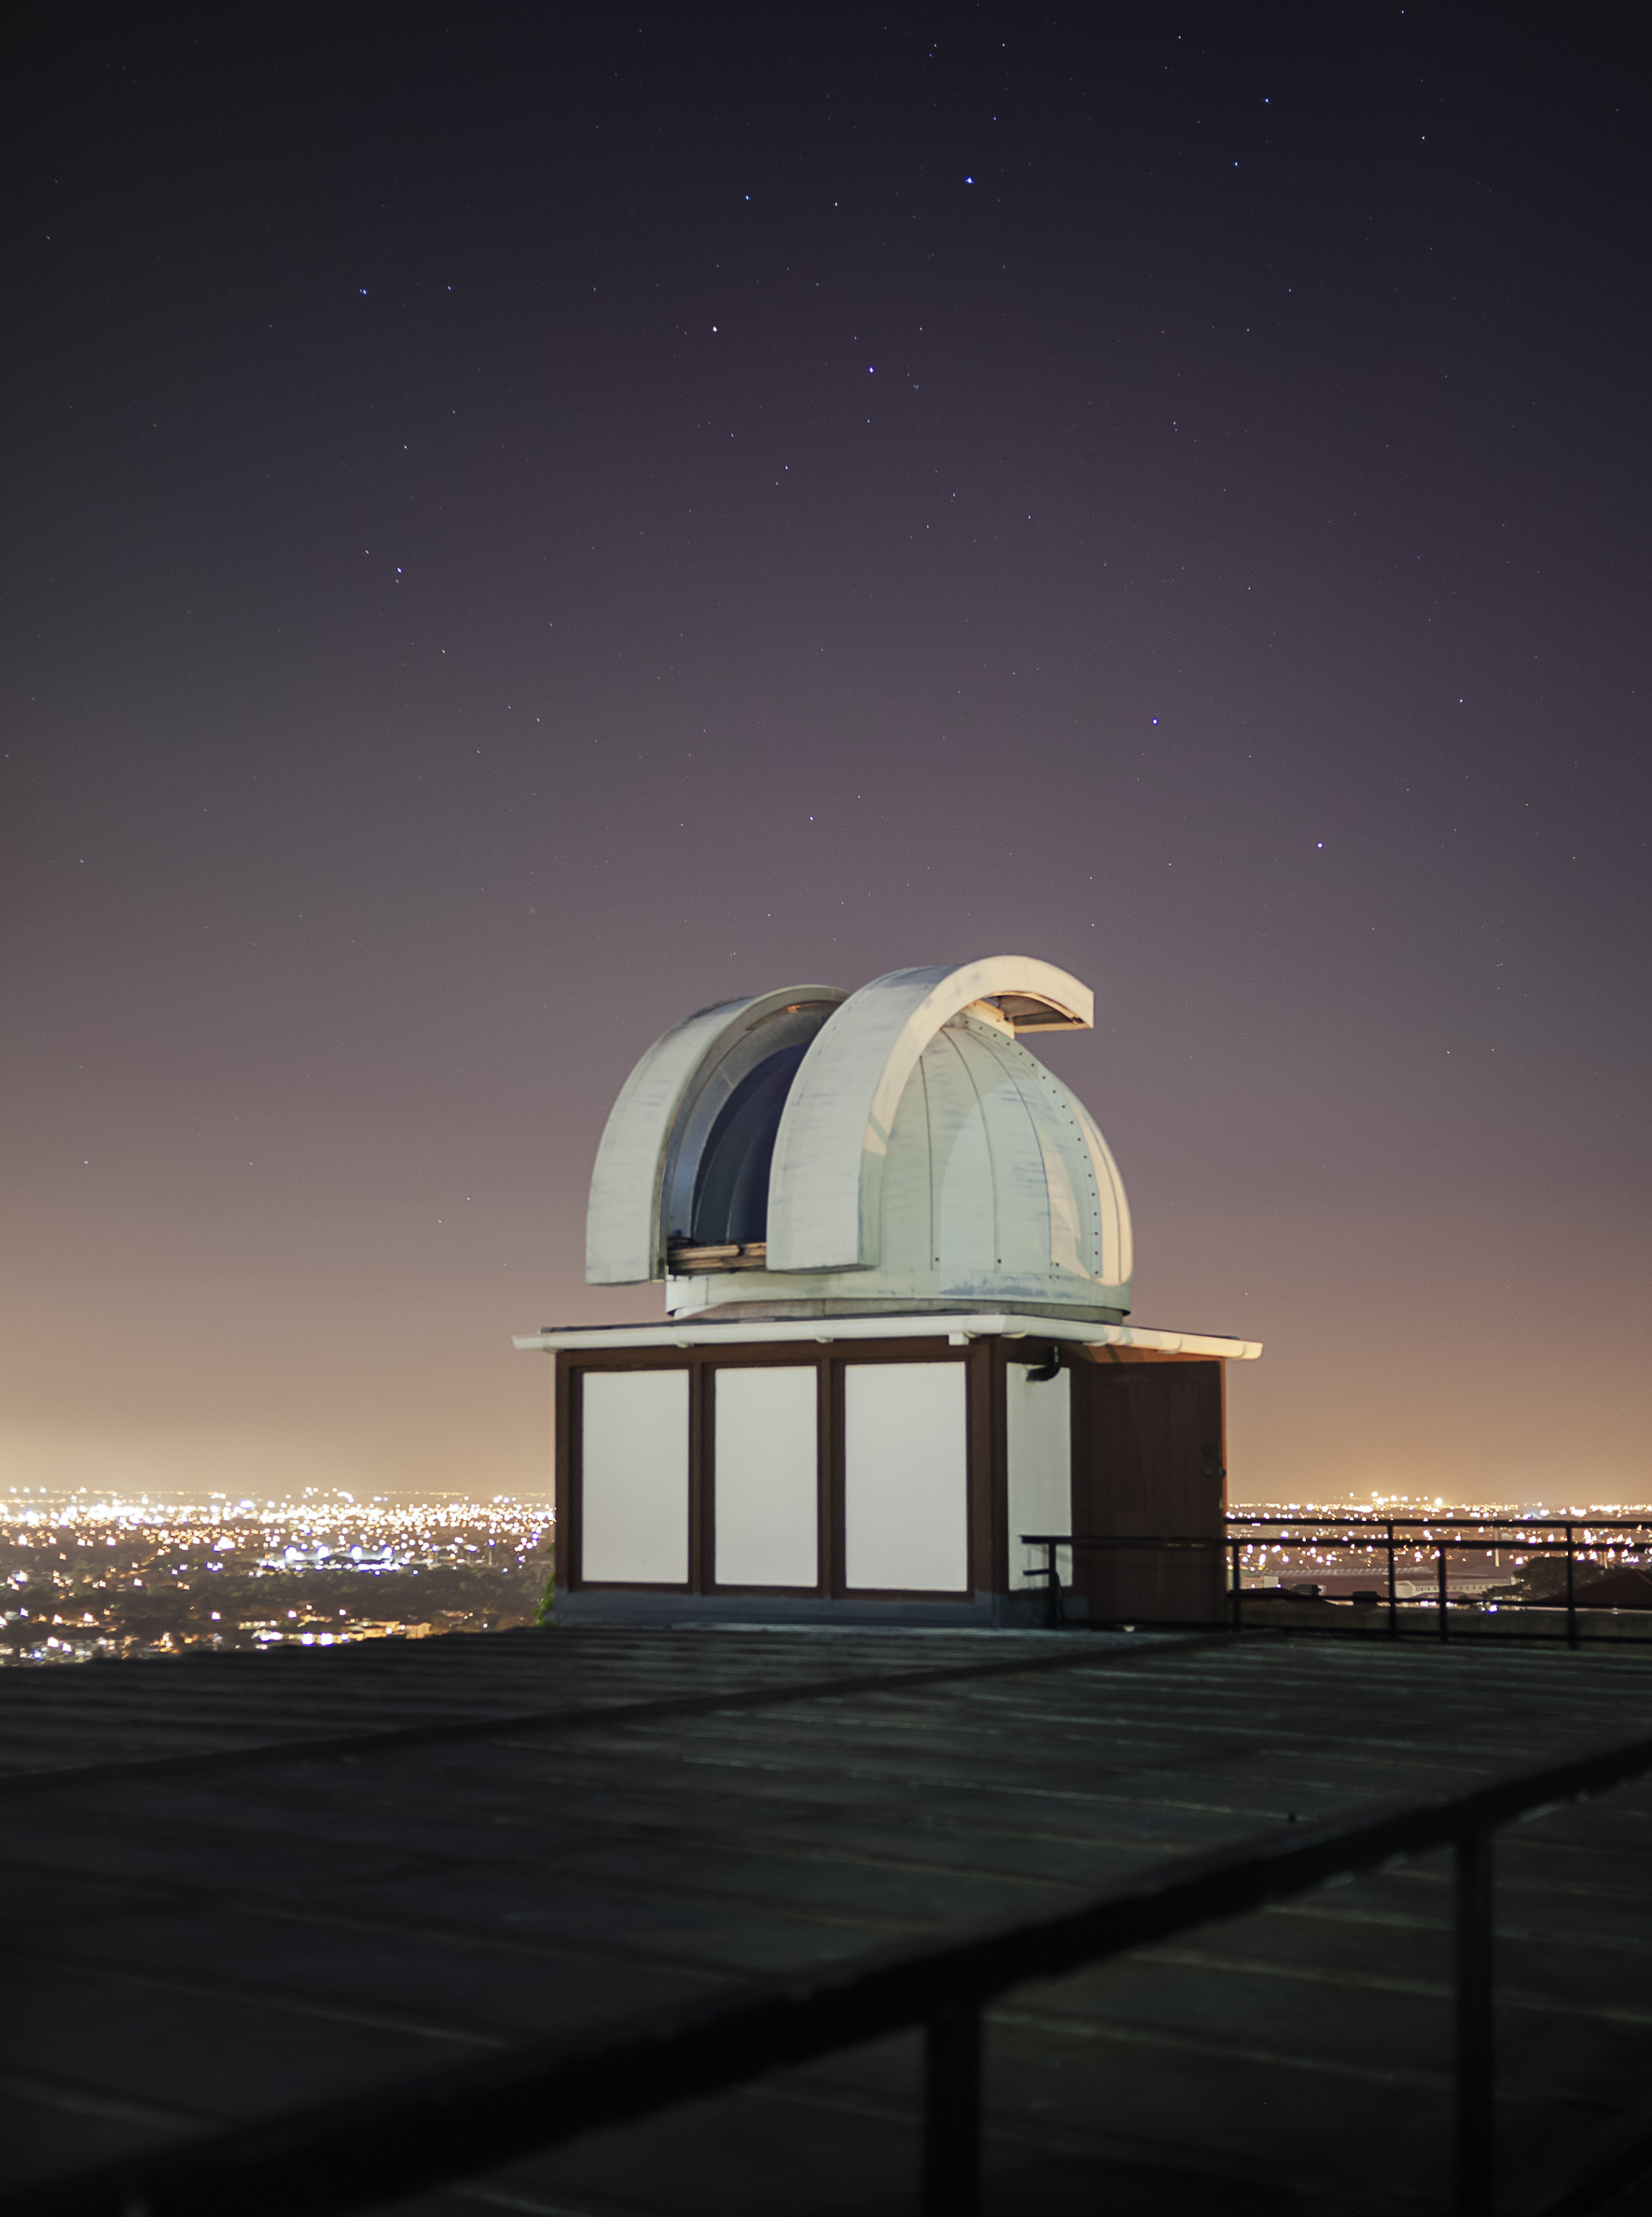
\includegraphics[width=13.5cm]{documentation_images/dome_at_night.jpg}

    \vspace{0.75cm}

    {\small Thuso Simon \& Charl Cater \& Patrick Woudt\\thuso@ast.uct.ac.za\\Version $0.3$a}
    \end{center}
    \vspace*{\fill}
  \end{titlepage}


\tableofcontents
\vspace{-10mm}




%--------------------------------
% The Observatory
%--------------------------------

\chapter{The Tony Fairall Teaching Observatory}

\begin{figure}[ht]
 \centering
    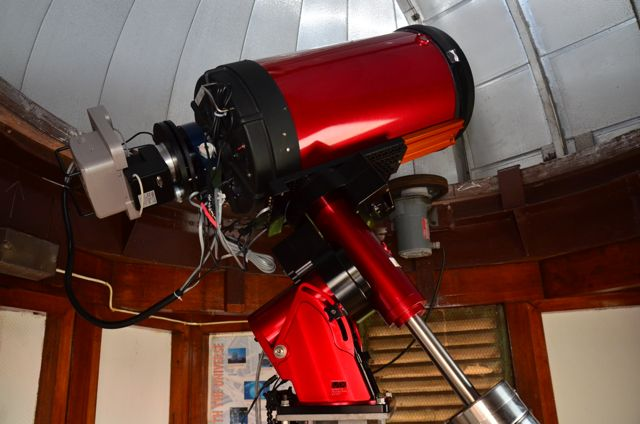
\includegraphics[width=0.75\textwidth]{documentation_images/telescope.jpg}
    \caption{\label{fig:telescope}The 14-inch Celestron telescope inside the observation dome.}
\end{figure}

This document is a user's guide to the 14-inch Celestron telescope and the accompanying suite of instruments housed at the Tony Fairall Teaching Observatory at the University of Cape Town. This is a modern telescope that is used for teaching and simple astronomy projects. This guide will 
help you to understand and use the telescope and highlights the operational procedures. Read this document
carefully to ensure the safe use of the telescope.\\

Previously known simply as the UCT Teaching Observatory, these facilities were dedicated to Professor A.P. (Tony) Fairall in 2013. Professor Fairall was a much respected astronomer and scientist, and was greatly revered for the passion and ease with which he brought astronomy to his students and the general public alike.\\

The observatory is located on the roof of the RW James building on UCT's Upper Campus. The GPS coordinates are $33 \,^{\circ}57'21.3''\mathrm{S}$ $18\,^{\circ}27'41.7''\mathrm{E}$ and the dome is approximately 120 meters above sea-level.\\

\textbf{Chapter 2} of this document describes all basic observing procedures, including the start-up and shut-down sequence,
the telescope control via dedicated software (\emph{The SkyX}), the CCD camera control via its dedicated
software (\emph{Maxim DL}), target acquisition and auto-guiding.\\

\textbf{Chapter 3} outlines a number of advanced observing procedures, including remote observing and details of 
instrument changes.\\

\textbf{Chapter 4} highlights general guidelines for photometry.\\

\textbf{Chapter 5} describes usage of the newly-commissioned spectrometer.\\

\vfill \eject




%--------------------------------
% Basic Observation Procedures
%--------------------------------

\chapter{Basic Observing Procedures}

\section{Start up procedures}

This chapter describes the basic observing procedures on the 14-inch UCT teaching telescope. 
Step-by-step instructions are given in this Section and
summarized in Section~\ref{checklists}.

\subsection{Connecting the laptop}

The first step is the connect the observatory laptop to the power socket and internet cable. Make
sure that the dome control USB and the telescope control USB cables are connected to the laptop.
Turn on all the power switches in the dome (on the East and North wall of the dome) and start the
(windows) laptop.

\begin{figure}[ht]
 \centering
    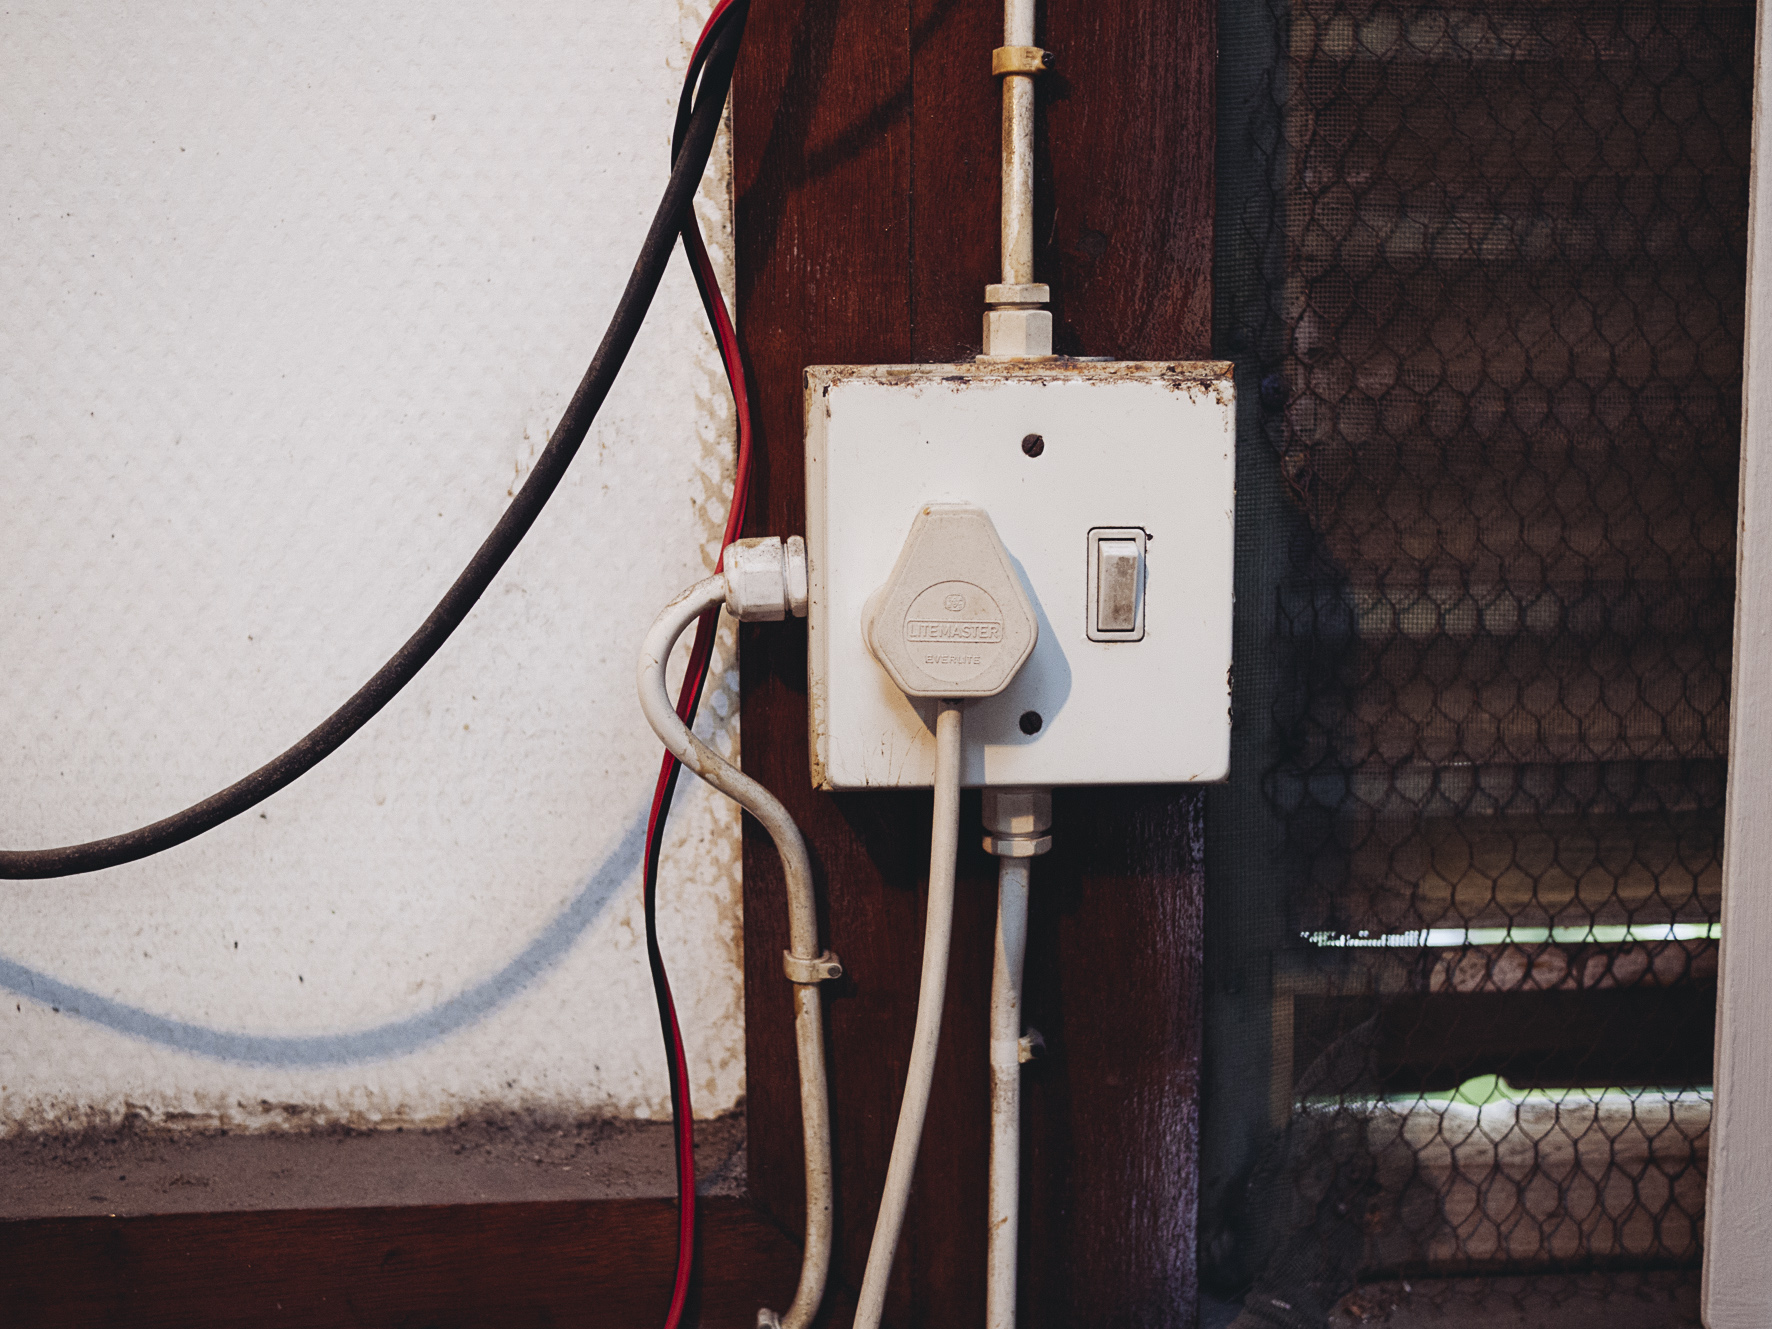
\includegraphics[width=0.49\textwidth]{documentation_images/plugs_E.jpg}
    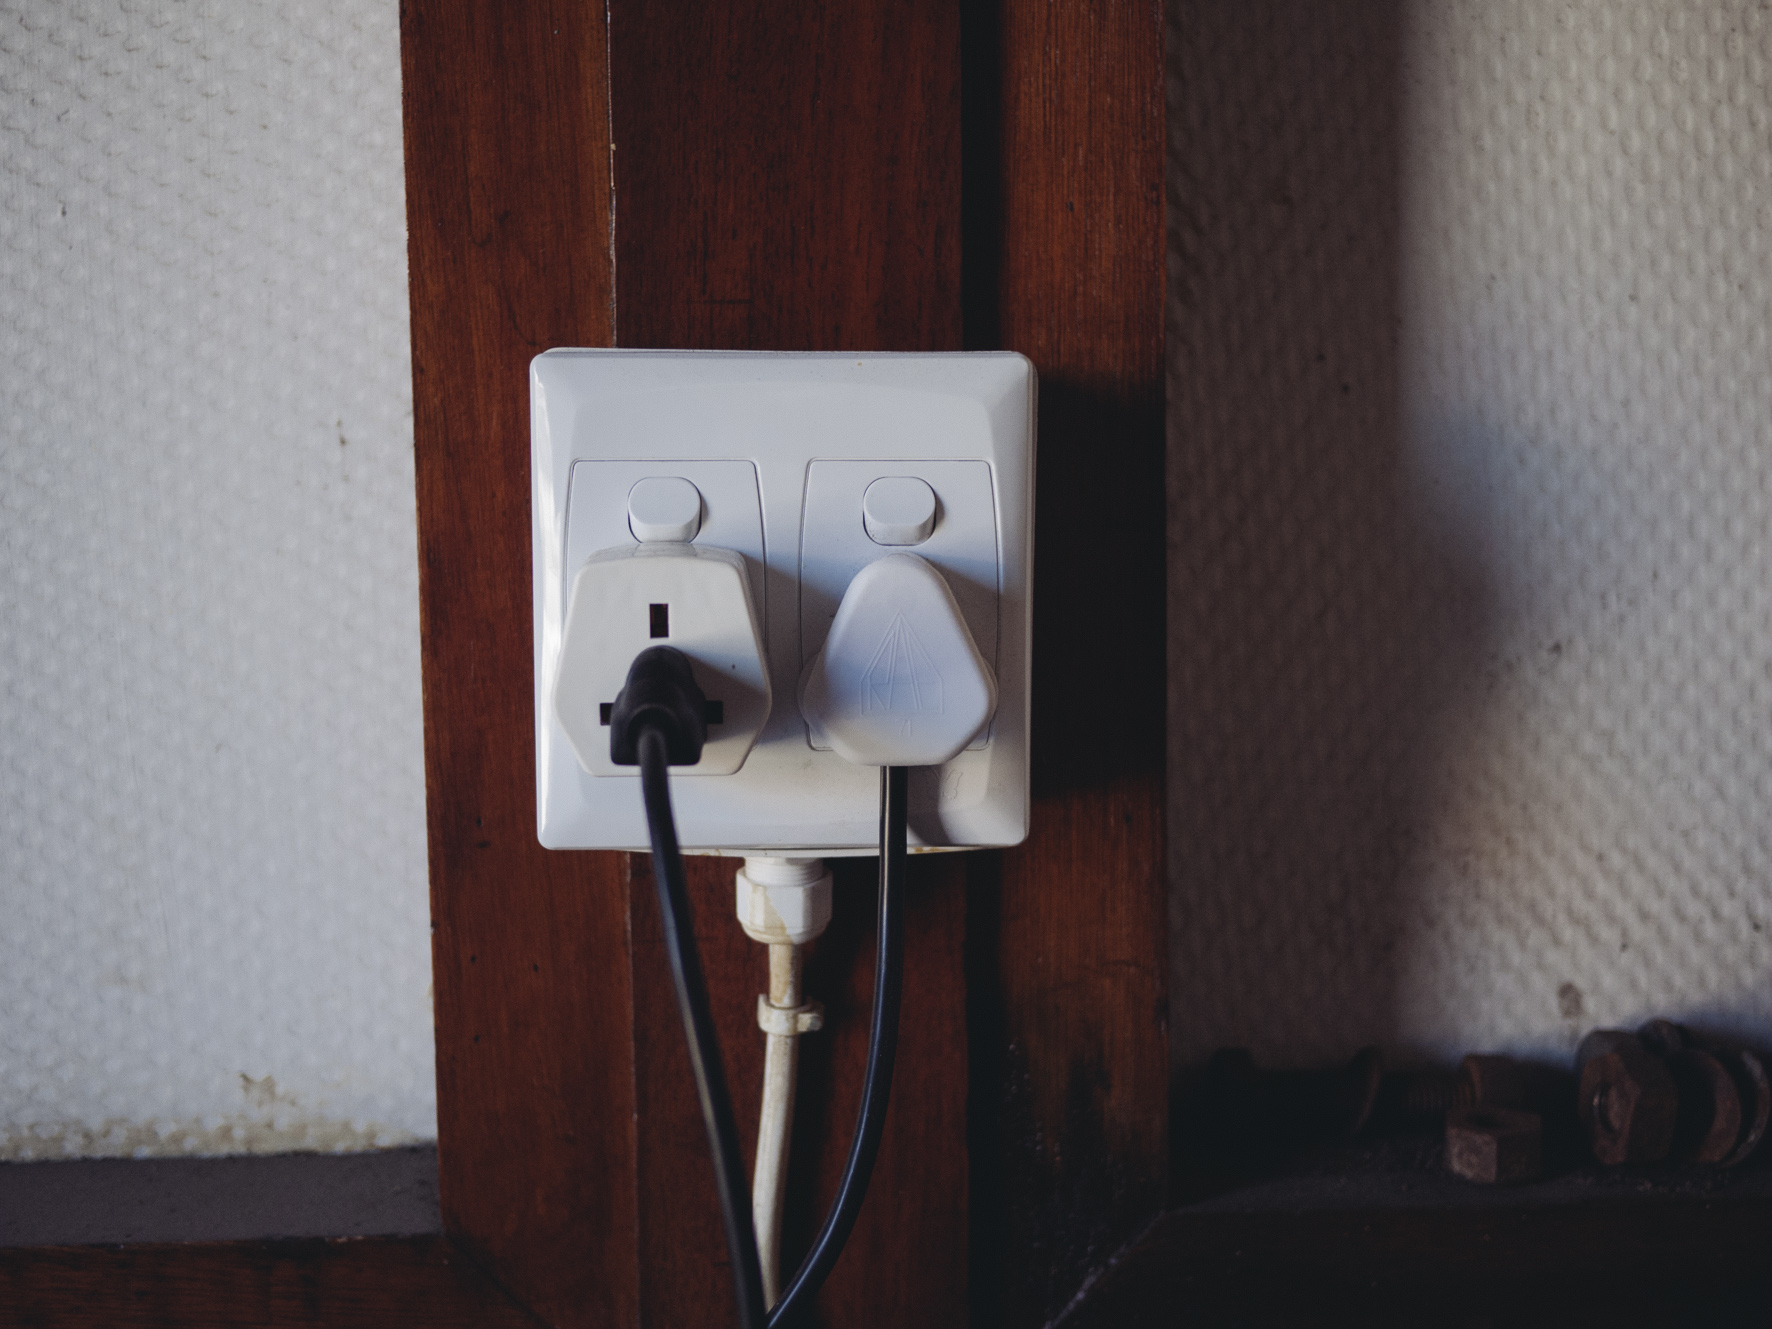
\includegraphics[width=0.49\textwidth]{documentation_images/plugsN_2.jpg}
    \caption{\label{fig:plugs}Switching on the power plugs. The left image shows the East wall plugs, the
image on the right shows the North wall plugs.}
\end{figure}

\subsection{Dome and telescope cover}

A sheet currently covers the telescope and protects it against dust. You can remove the sheet at this point.
In order to avoid damage to the telescope mirror from anything falling down whilst opening the dome, 
it is important to \emph{first} open the dome (at present this requires a bit of elbow grease), after which 
you can remove the telescope cover.\\

\subsection{The pull test}
To be sure that none of the instruments attached to the telescope might fall off and get damaged during the observation, it is recommend that you do a quick `pull test': Hold on firmly to the CCD imager or spectrograph at the back of the instrument stack and give a firm tug (in the direction away from the telescope) to check that it is fastened securely.

\subsection{Unlocking the RA and DEC drives}

When the telescope is parked during the day, both the Right Ascension (RA) and Declination (DEC) drives are 
in a `locked' position, ensuring the telescope does not move when there is no power to the telescope.\\

At this stage of your observing session, you now need to put the RA and the DEC drive from a 'locked' position
to a `star' position. This enables the telescope drive to be controlled from the laptop. 
Notice that when the drive clamps are in the mid position (marked by a `balance' sign), the telescope 
can move freely. Be careful to gently hold/support the telescope when you switch the drives from 
lock to star position!

\begin{figure}[ht]
 \centering
    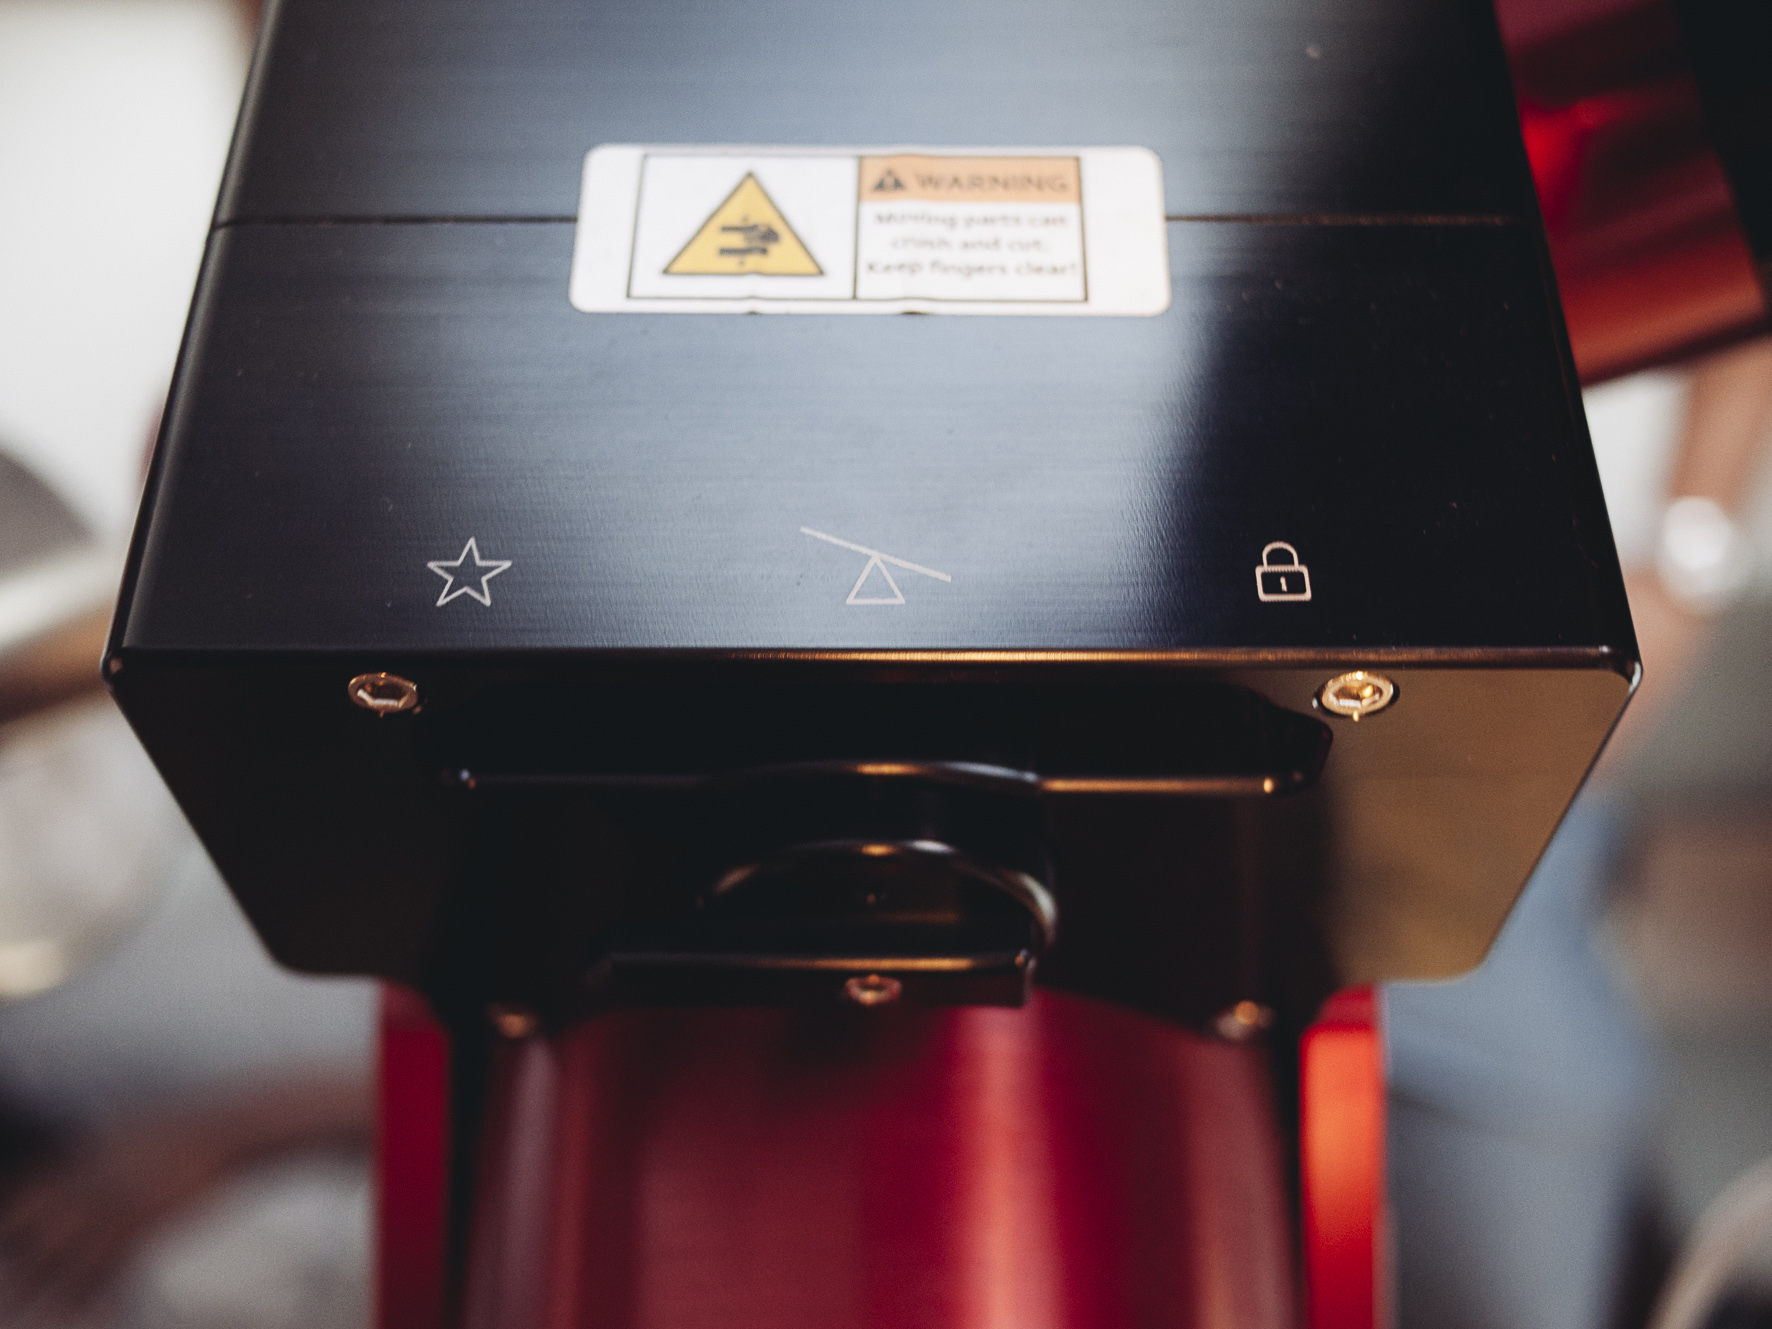
\includegraphics[width=0.49\textwidth]{documentation_images/drive_Dec}
    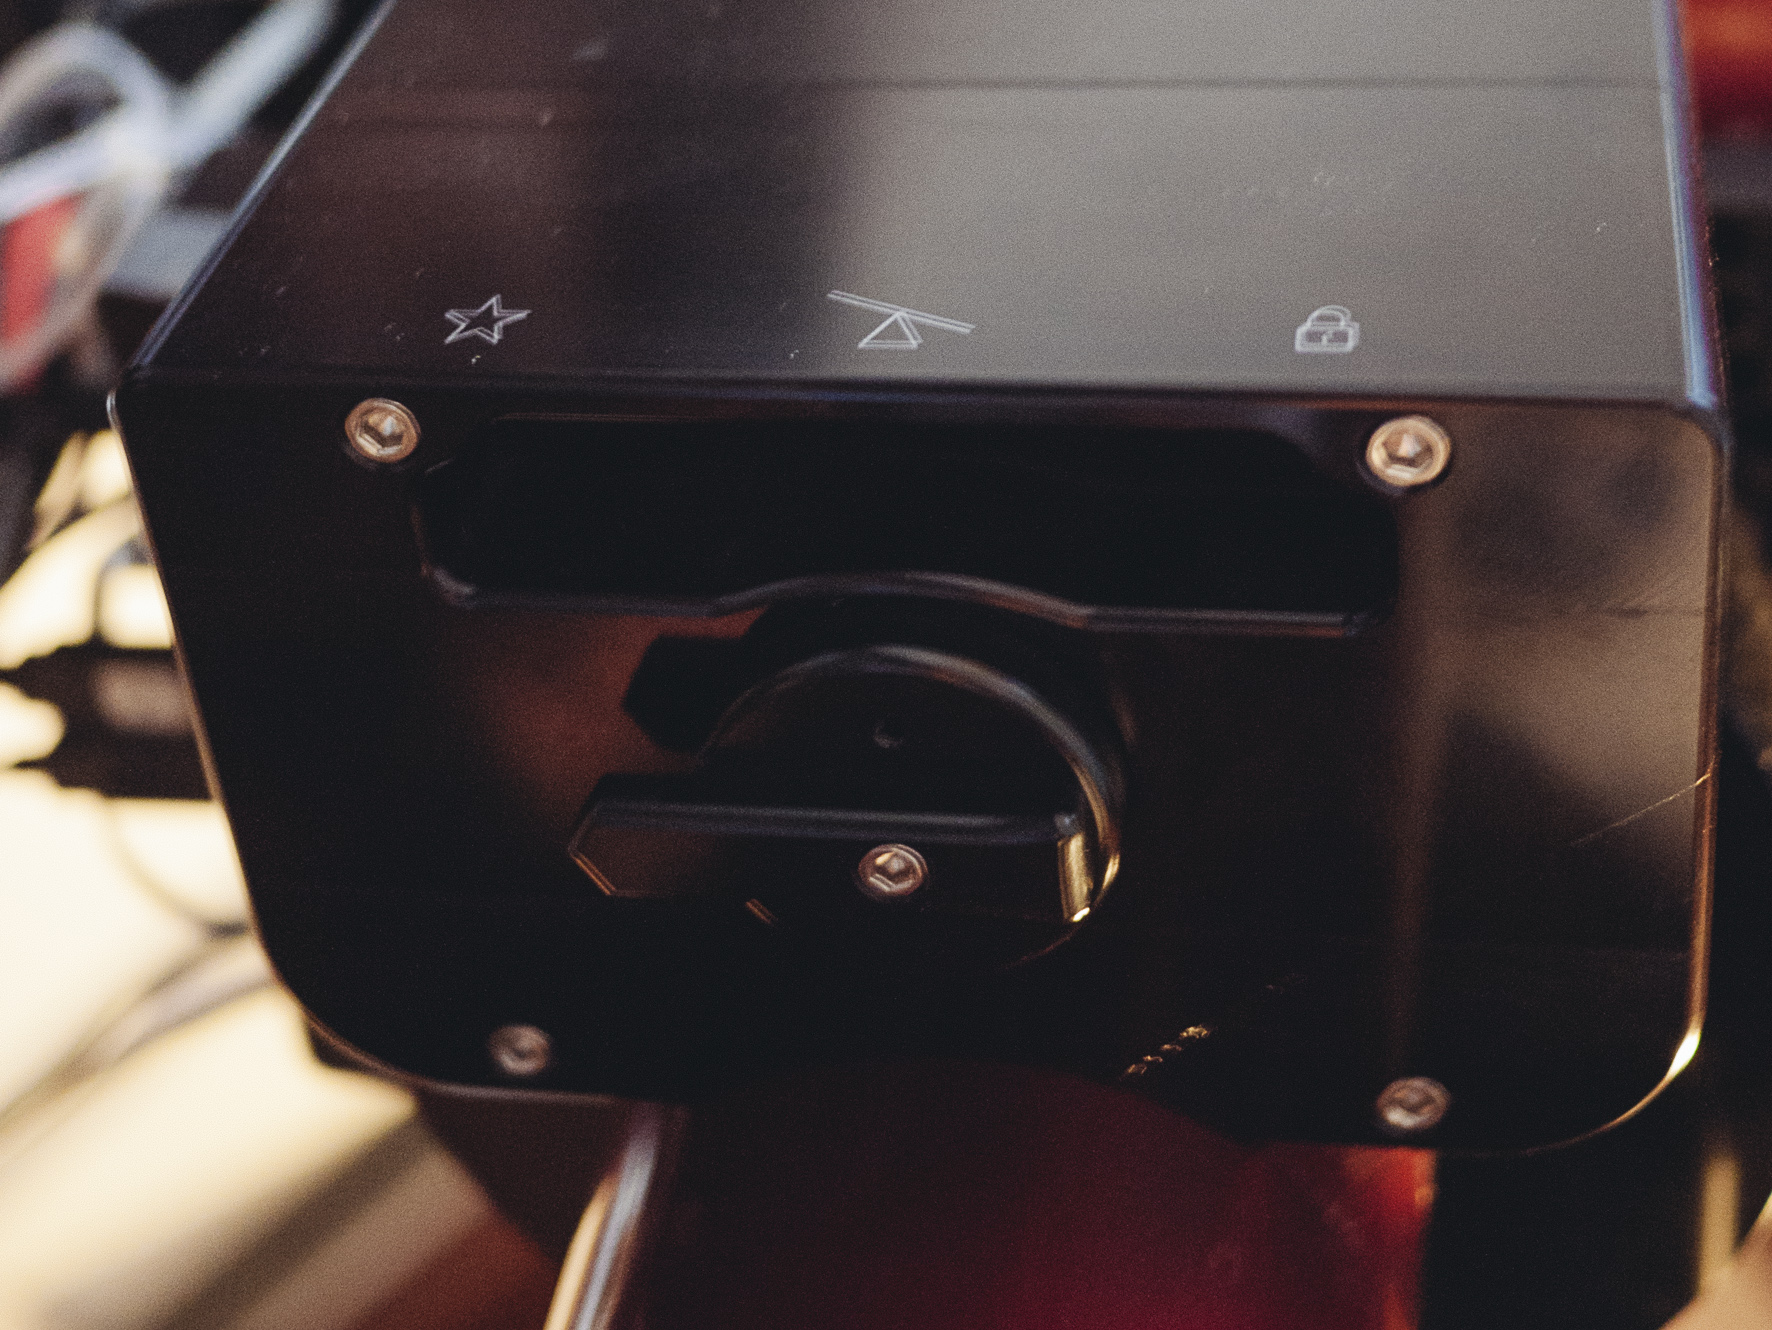
\includegraphics[width=0.49\textwidth]{documentation_images/drive_RA}
    \caption{\label{fig:drives}Left: Declination drive, right: Right Ascension drive.}
\end{figure}

\subsection{Telescope control: \emph{The SkyX}}
\label{telescope_control}

\emph{The SkyX} is an all inclusive astronomy program that gives you the power of the 
universe at the point of a mouse. It should be able to guide the telescope, control the CCD, 
focus the image, control the dome and control the rotator. 
Unfortunately, it has some bugs so all it can really control at the moment the telescope, the 
dome rotation and the CCD rotator. To access the user manual for \emph{The SkyX}, 
visit \url{http://www.bisque.com/help/TheSkyXSAEAndPro/index.htm}.\\

On the laptop you can start \emph{The SkyX}. This program controls the telescope, the dome and the
rotator (on which the CCD is mounted).\\

You will see a big X symbol on the laptop for 'The SkyX Professional Edition'. Double click this
system to start \emph{The SkyX}. You can minimize the window during the observations if you need to 
toggle between telescope control and CCD control. You can reopen the window by clicking on the 'X' 
on the bottom bar.\\

During the start up procedure you need to \textit{connect} and \textit{Find Home} for the dome, 
the telescope and the rotator. To connect the telescope, click on the \textbf{Telescope} bar on the left-vertical menu, and 
under the \textbf{Start Up} pull-down menu, select \textbf{Connect}. The program will then request 
a \textit{Find Home} procedure, which will initialize the telescope.\\

%\clearpage

Before you enable the \textit{Find Home} procedure, make sure to remove any chairs or other obstacles that might be in the
way of the telescope as it moves. Confirming the \textit{Find Home} command will move the telescope 
to its start-up position. The status should read: {\textcolor{PineGreen}{\tt Tracking at sidereal rate}}.
The display of \emph{The SkyX}, \textit{connecting} the telescope is shown in 
Figure~\ref{fig:connect_telescope}.\\

\begin{figure}[ht]
 \centering
    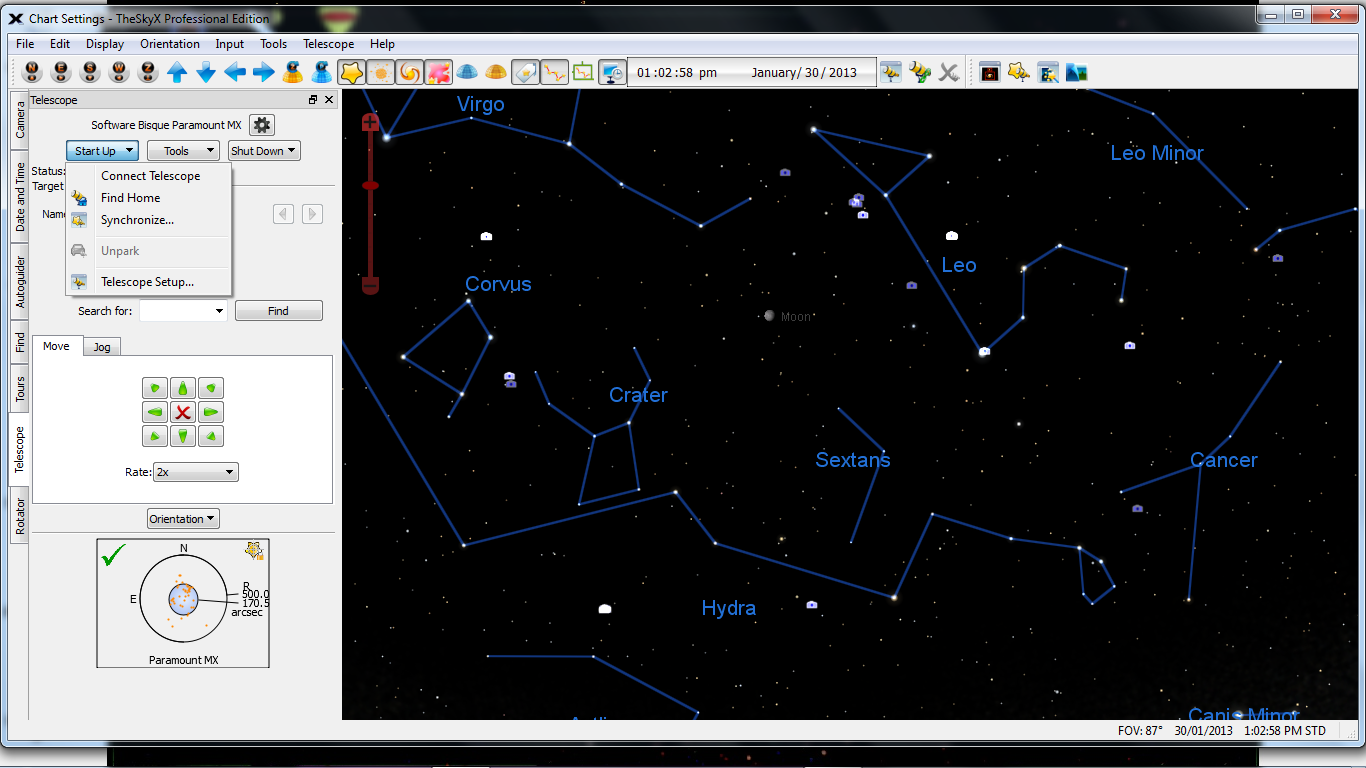
\includegraphics[width=0.75\textwidth]{documentation_images/connect_telescope.png}
    \caption{\label{fig:connect_telescope}Shows how to connect the computer to the telescope.}
\end{figure}

Next, to connect the dome, click on the \textbf{Dome} bar on the left-vertical menu and press 
\textbf{Connect}. The status of the dome should now read: \textcolor{PineGreen}{\tt Connected}.
To connect the rotator, click on the \textbf{Rotator} bar on the left-vertical menu and 
click \textbf{Connect}. Repeat this if \emph{The SkyX} complains.  The status of the Rotator should 
read: \textcolor{PineGreen}{\tt Ready}. The telescope is now ready for use.\\

\begin{figure}[ht]
 \centering
    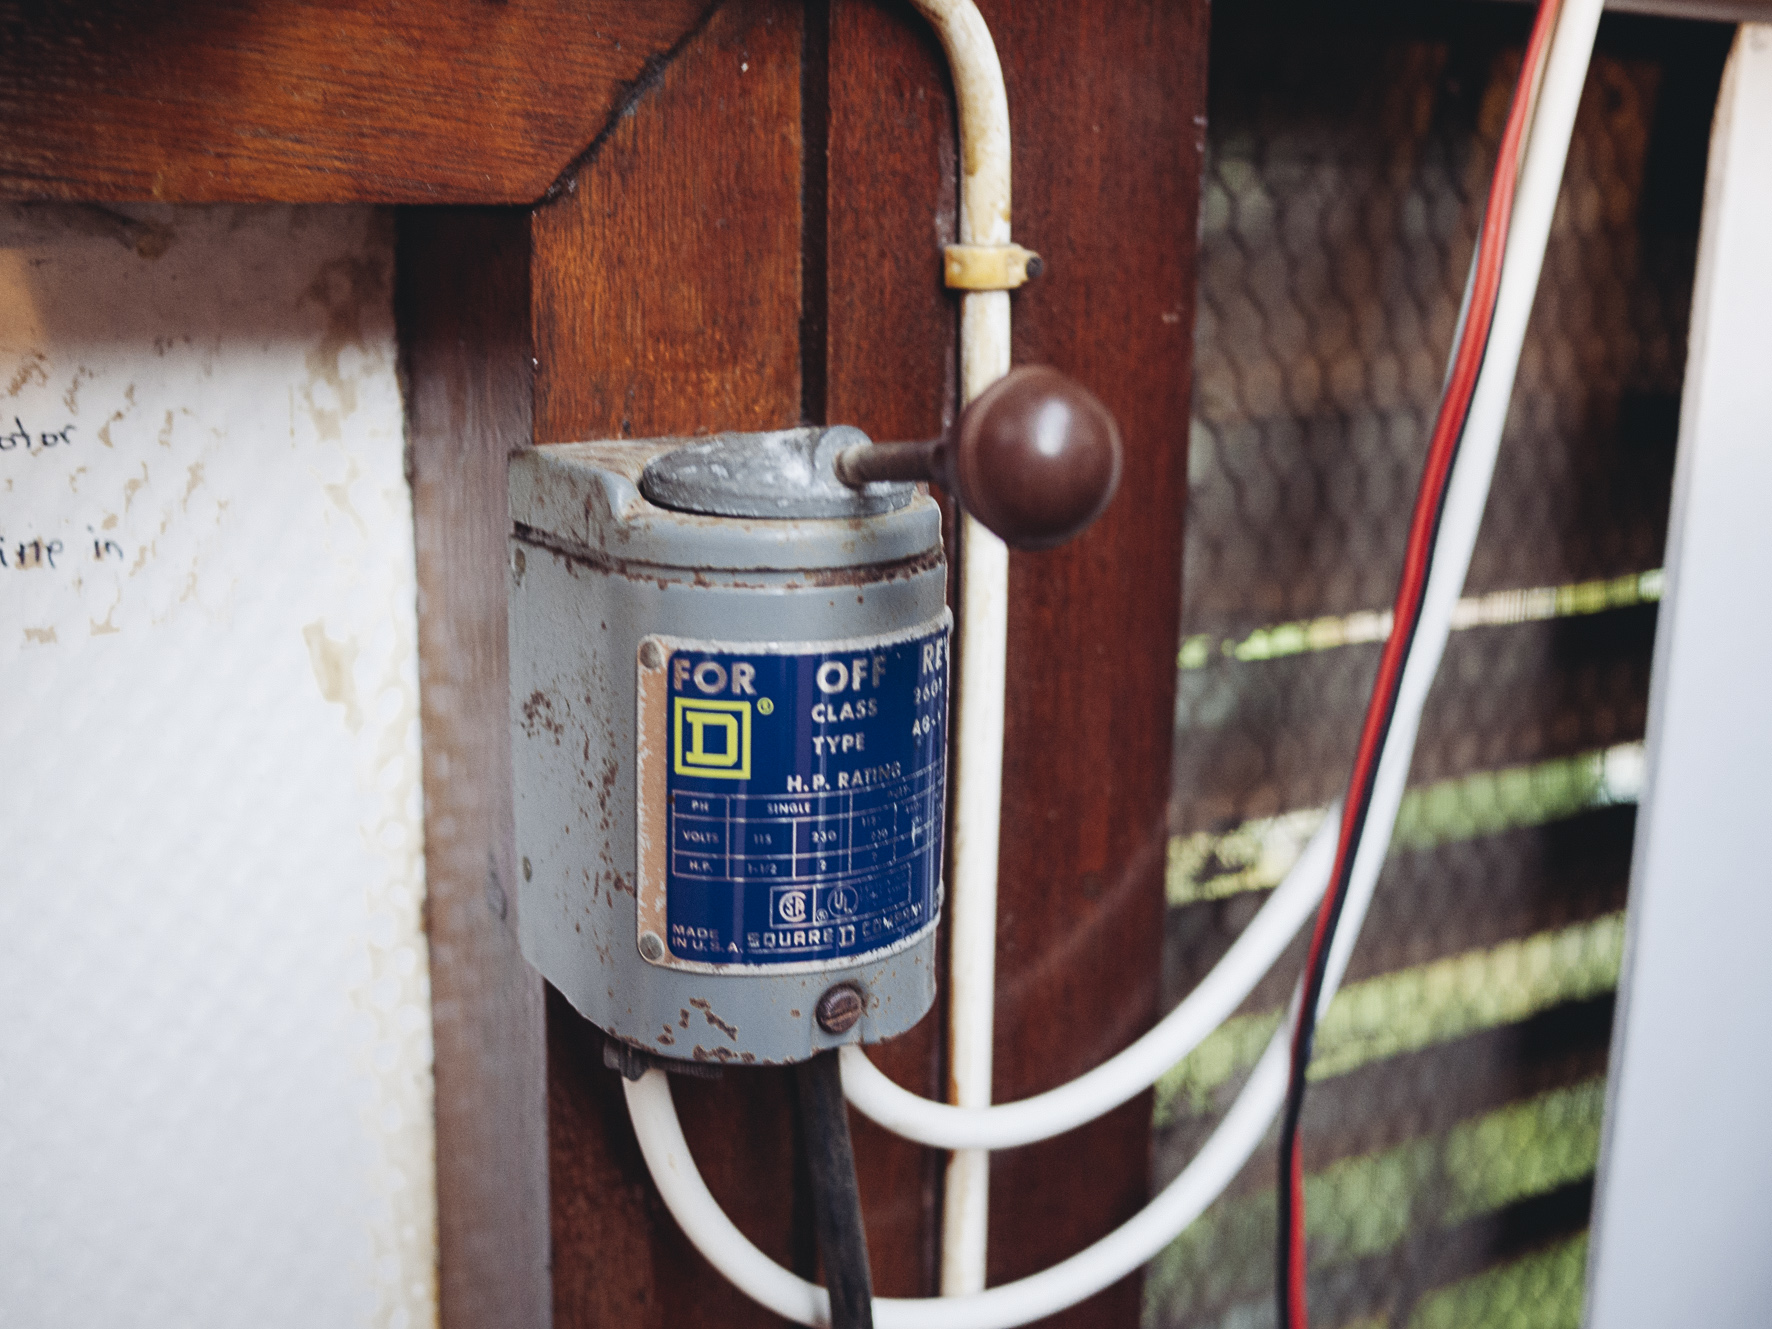
\includegraphics[width=0.75\textwidth]{documentation_images/dome_control.jpg}
    \caption{\label{fig:dome_control}Manual override lever for the dome.}
\end{figure}

The motor that controls the Dome's rotation is slightly more powerful than necessary, so the dome may occasionally overshoot in such a way as to block the telescope's view. To rotate the dome back into place, the lever seen in Figure~\ref{fig:dome_control} was installed on the East wall of the room. Pushing the lever to the left (FOR) will move the Dome anti-clockwise and to the right (REV), clockwise. Use this lever when you see that the dome-opening is not aligned with the telescope's pointing and needs adjustment.\\


\subsection{CCD control: \emph{Maxim DL}}

On the laptop you can start \emph{Maxim DL}. Double click on the symbol for 'Maxim DL Pro 5'. 
Minimization of the window is the same as for \emph{The SkyX}.\\

To enable CCD camera control from the laptop, click on the \textit{Toggle Camera Control (CTRL + W)} button.
This button is located in the second row of the menu bar and looks like a `button with two wires'. 
This will open a new window (entitled \emph{Camera Control}, see Figure~\ref{fig:coolers}).  
In this window, click \textbf{Connect}.\\

A new window is launched (entitled \emph{SBIG AO Control}). On the `Camera Control' window, click on
coolers \textbf{On}. This will cool the CCD-chip in the camera. You will notice that the temperature for 
Camera 1 (the normal CCD) will drop to $-5 \,^{\circ}\mathrm{C}$ (a preset temperature that depends on the outside 
temperature).\\

\begin{figure}[ht]
 \centering
    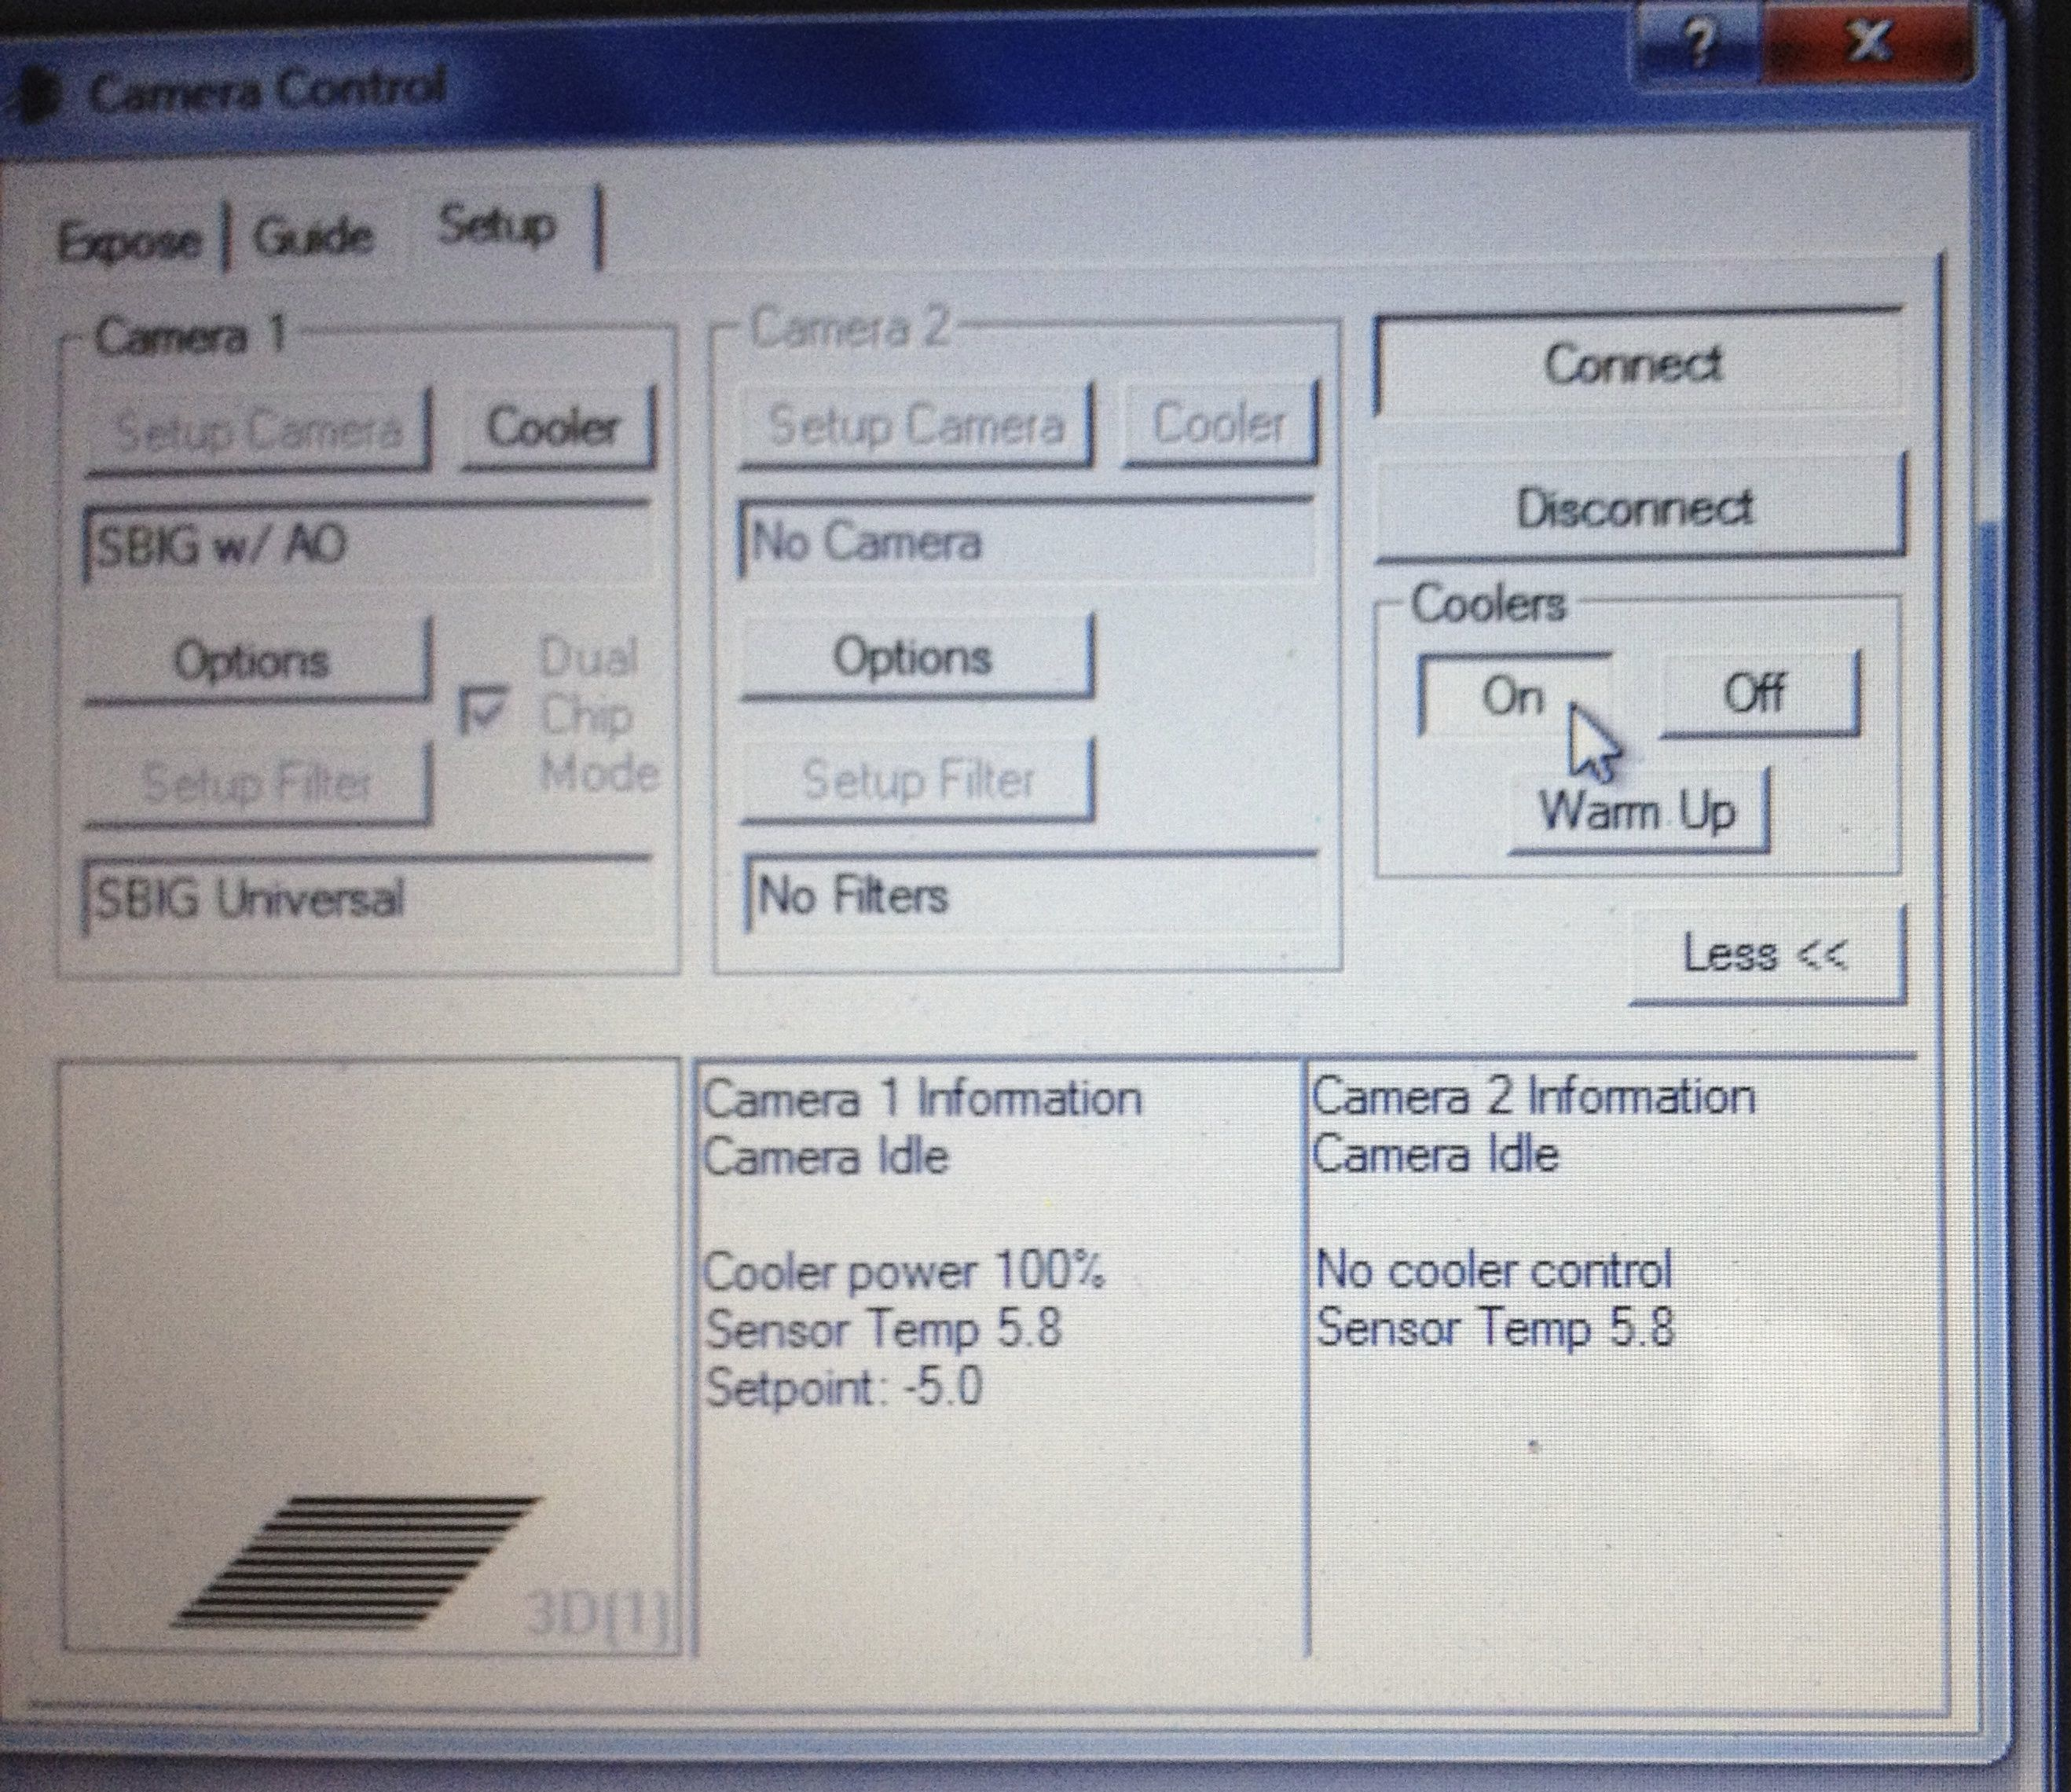
\includegraphics[width=0.49\textwidth]{documentation_images/maximdl_cooler}
    \caption{\label{fig:coolers}The camera control window on \emph{Maxim DL}.}
\end{figure}

Once the sensor temperature is down to the set-point temperature, the CCD camera is ready for use. 
The cooling power should be around 60-70\%. If it is persistently above 70\%, change the set-point 
temperature to a higher value (in steps of $5 \,^{\circ}\mathrm{C}$) through the `Setup' button.\\

The entire system is now ready for on-sky observations, align the pointing and setting the focus of the telescope. From there you can acquire your science target and set up the auto-guiding using the 'Adaptive Optics' module (Camera 2 in \emph{Maxim DL}). This process is described in the following two sections.

\section{Acquiring a target}
\label{acquire}

% \begin{figure}[h]
% \centering
%    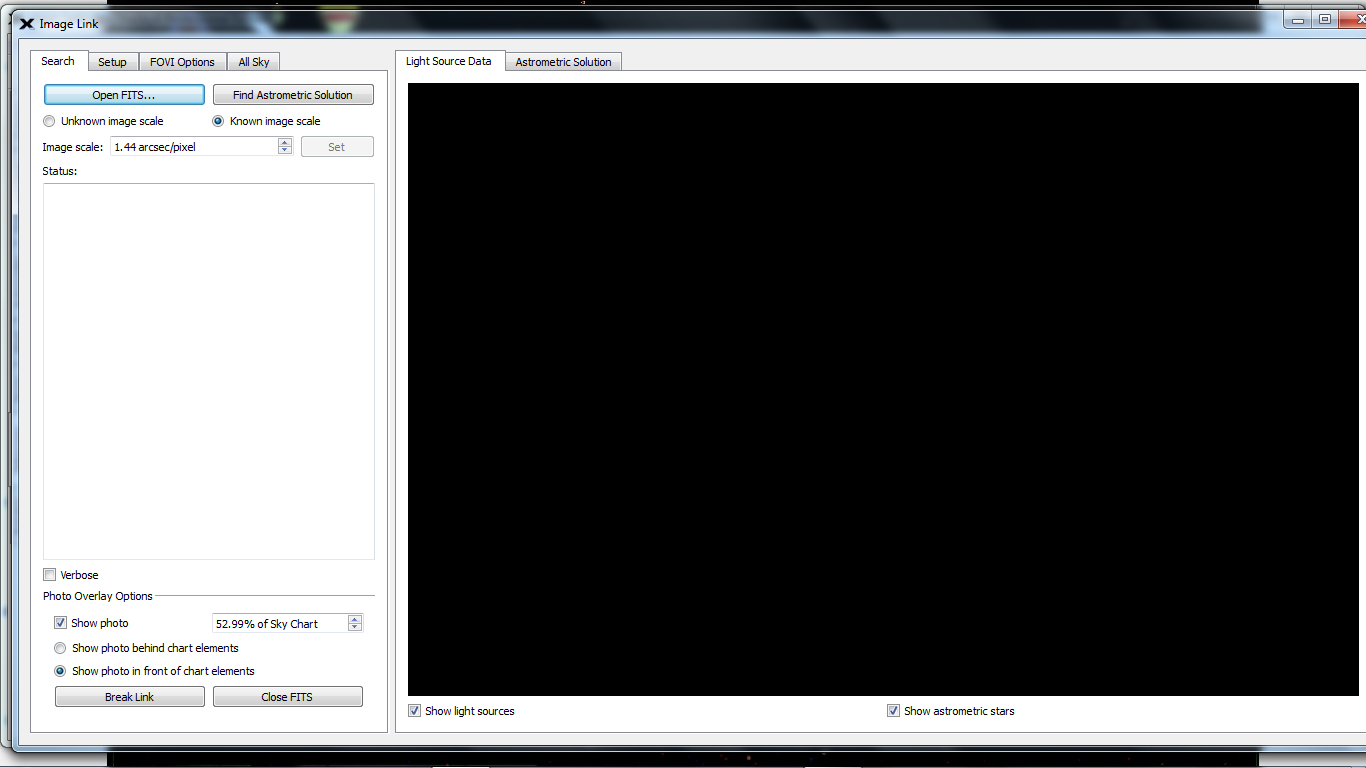
\includegraphics[width=\textwidth]{documentation_images/basic_interface.png}
%    \caption{\label{fig:basic_interface} This is how \emph{The SkyX} looks like when it is open.}
% \end{figure}

\subsection{Aligning the pointing of the telescope}
\label{pointing}

%\subsection{Small Changes to Pointing}
%\label{small_changes_to_pointing}

If the telescope and the \emph{The SkyX}'s pointing are not precisely aligned, follow these steps to correct it. 

\begin{enumerate}
 \item Find and slew to field you would like to look at.

 \begin{figure}[ht]
 \centering
    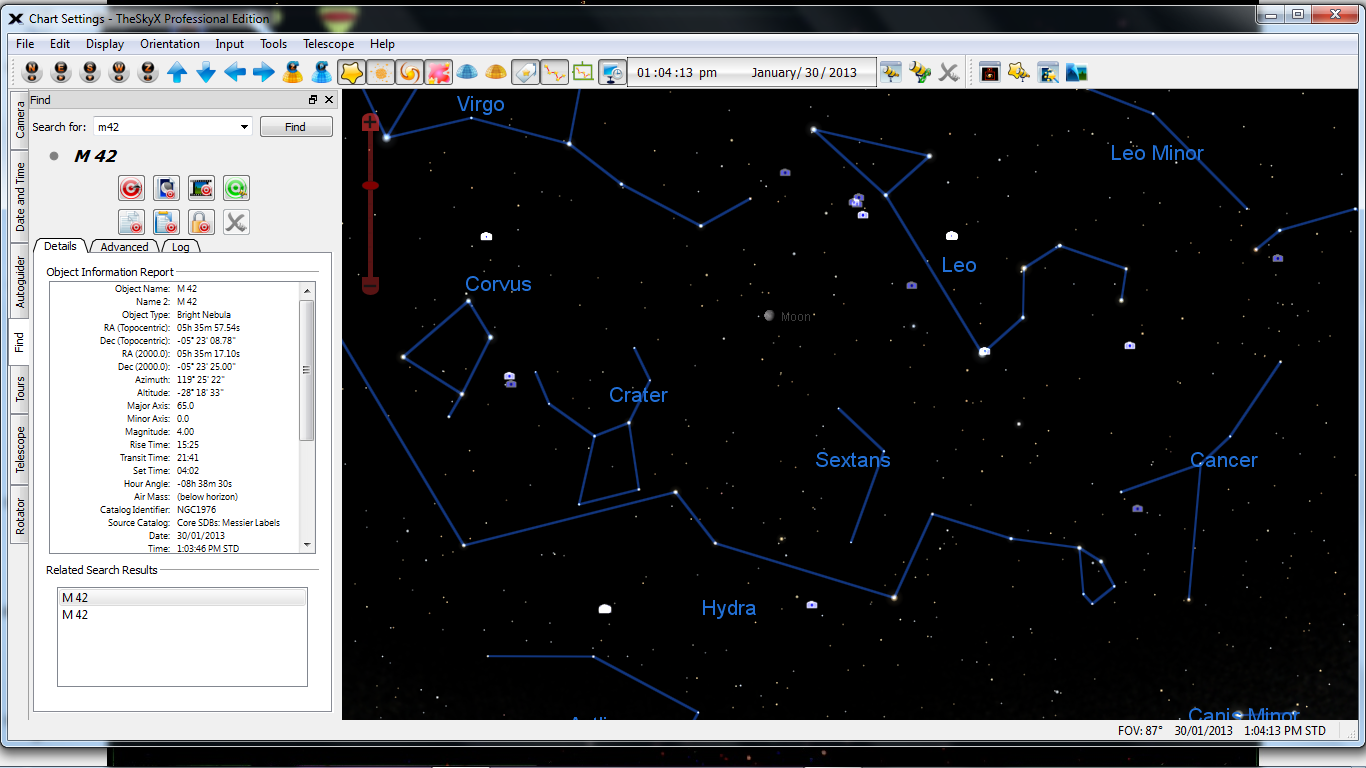
\includegraphics[width=0.75\textwidth]{documentation_images/moving_telescope.png}
    \caption{\label{fig:moving_telescope}Click the green slew button to start the telescope's movement.}
\end{figure}

 \item \label{2} Take an image with your favorite CCD manager, \emph{Maxim DL} for instance, and save the resulting .FITS file. (Note: For an astrometric solution like we are about to attempt, \emph{The SkyX} recommends using an image that contains at least eight distinct stars, so try to aim for a well-populated field).

 \item In \emph{The SkyX}, under the menu \emph{Tools -- Image Link} (Ctrl+Shift+I), in the \emph{Search} tab, click the \textbf{Open FITS...} window.

  \begin{figure}[ht]
 \centering
    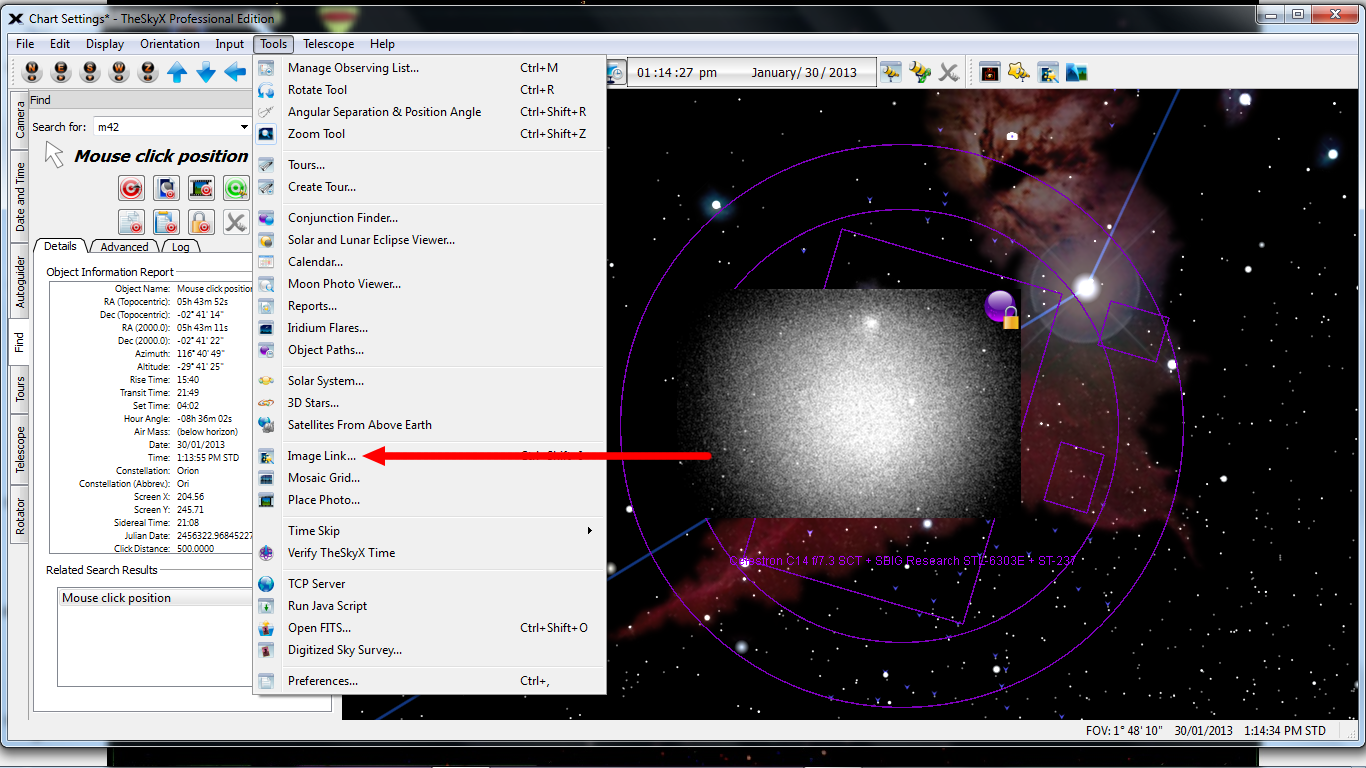
\includegraphics[width=0.75\textwidth]{documentation_images/tools_menu_1_1.png}
    \caption{ \label{fig:tools_menu}Click on \emph{Tools -- Image Link...} to access the image linking window.}
  \end{figure}

 \item Load in your saved test field from Step \ref{2} and then click the \textbf{Find Astrometric Solution} button. \emph{The SkyX} will now attempt to find the exact location of your photo on the sky. 

 \item If the solution fails, check that the binning and Image Scale of your loaded image is set correctly. They should be (for $x \times x$ binning):

 \begin{itemize}
  \item $1\times1 = 0.72$ arcseconds
  \item $2\times2 = 1.44$ arcseconds
  \item $3\times3 = 2.15$ arcseconds
  \item $4\times4 = 2.88$ arcseconds 
 \end{itemize}

 \item If you managed to obtain a successful solution , go to the \emph{FOVI Options} tab and click the \textbf{Synchronize Rotator Angle to Position Angle} button.

  \begin{figure}[ht]
 \centering
    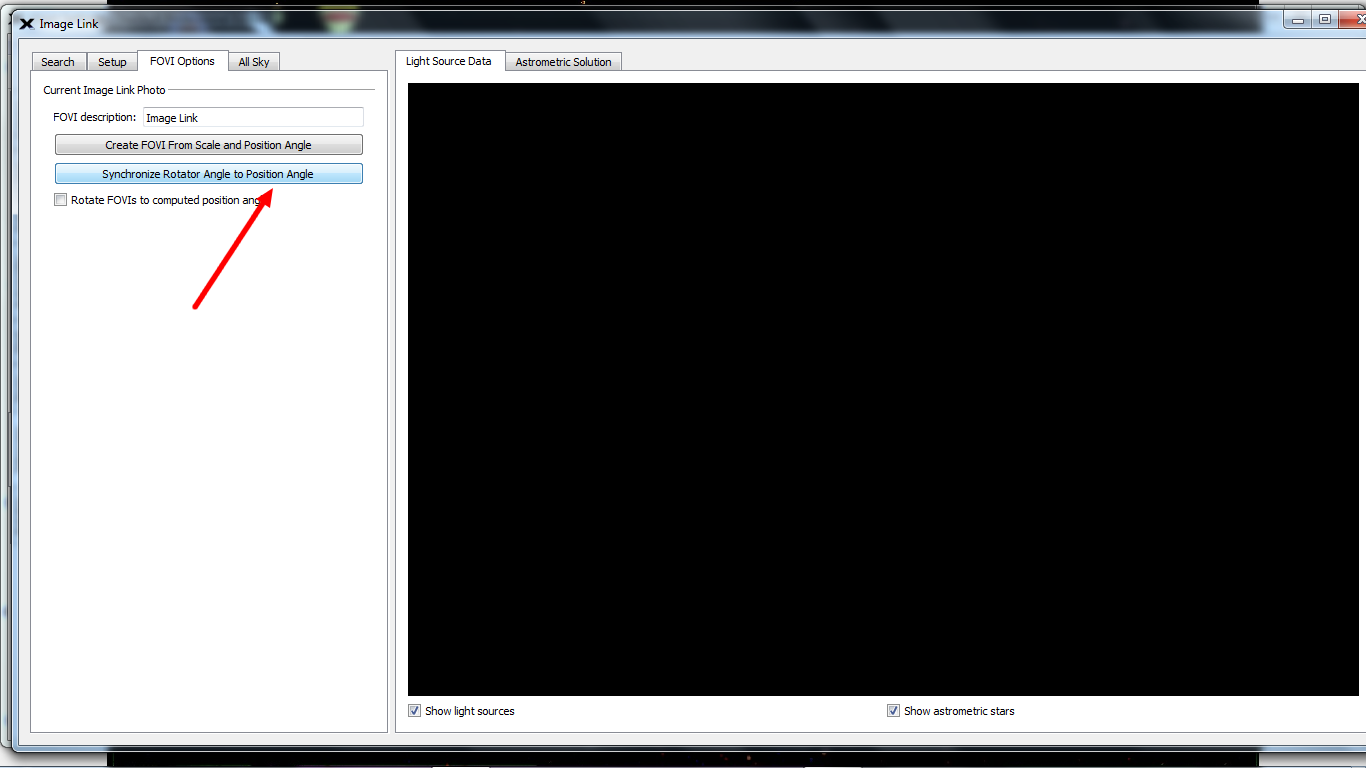
\includegraphics[width=0.75\textwidth]{documentation_images/pointing2_1.png}
    \caption{\label{fig:pointing1}Click at arrow to access sync telescope pointing with image.}
  \end{figure}

 \item Exit the Image Link window and go back to the main screen.

 \item Click on the loaded image in the main window until the heading in the \emph{Find} tab shows `Linked Photo'. This is to make sure you haven't mistakenly selected a star or other sky object other than your loaded image.

 \item Now click on the \textbf{Sync} button on the tool-bar. If all went well the telescope and the software should be pointing in the same direction now. If you find that the pointing is still misaligned, you may need to repeat steps 1 to 8. Repeated failures may also mean that some of the \emph{Source Extractor} parameters may need to be adjusted. For help with this, see the user's guide for \emph{the SkyX}.
\end{enumerate}

%\subsection{Rotator}
%\label{Correcting_rotation}

\emph{The SkyX} can control the rotation of the camera, but there is a bug in the software that causes the readings to be off, and this changes depending on where you are pointing in the sky. There is also no easy way to adjust the rotation of the CCD in \emph{The SkyX}.\\

\clearpage

The rotator is important for selecting a guide star for the Adaptive Optics (AO). The following steps tell you how to calibrate and align a guide star on the AO CCD.
\begin{enumerate}
 \item Step 1
 \item Step 2
 \item Step 3
 \item Step 4
 \item Step 5: Get coffee, repeat.
\end{enumerate}


\subsection{Focussing the telescope}
\label{focussing}

From time to time the telescope will need to be refocused. This is especially true when changing between instruments (since the focus points of these instruments are located at different distances from the back of the telescope), but may even be necessary when changing to a different filter. This section will describe how to find the optimal focus.

\begin{enumerate}
 \item Start by slewing to a field that has at least one star (that is not too bright, but also not too dim; ideally between magnitudes 7.5 - 9), which you can can use to focus on.
 \item In the `Camera' window in \emph{Maxim DL}, select the \textbf{Focus Tools} tab. 
 \item Deselect the options for taking dark and sub-frames and automatically saving focus photos; and select the option to `Take Photo Continuously'. Make sure you'll be taking `Light' frames by selecting the correct option from the drop-down menu.
 \item Set an appropriate exposure time (somewhere between 3 and 5 seconds will usually work) and press the \textbf{Continuous Photos} button.

 \begin{figure}[ht]
  \centering
    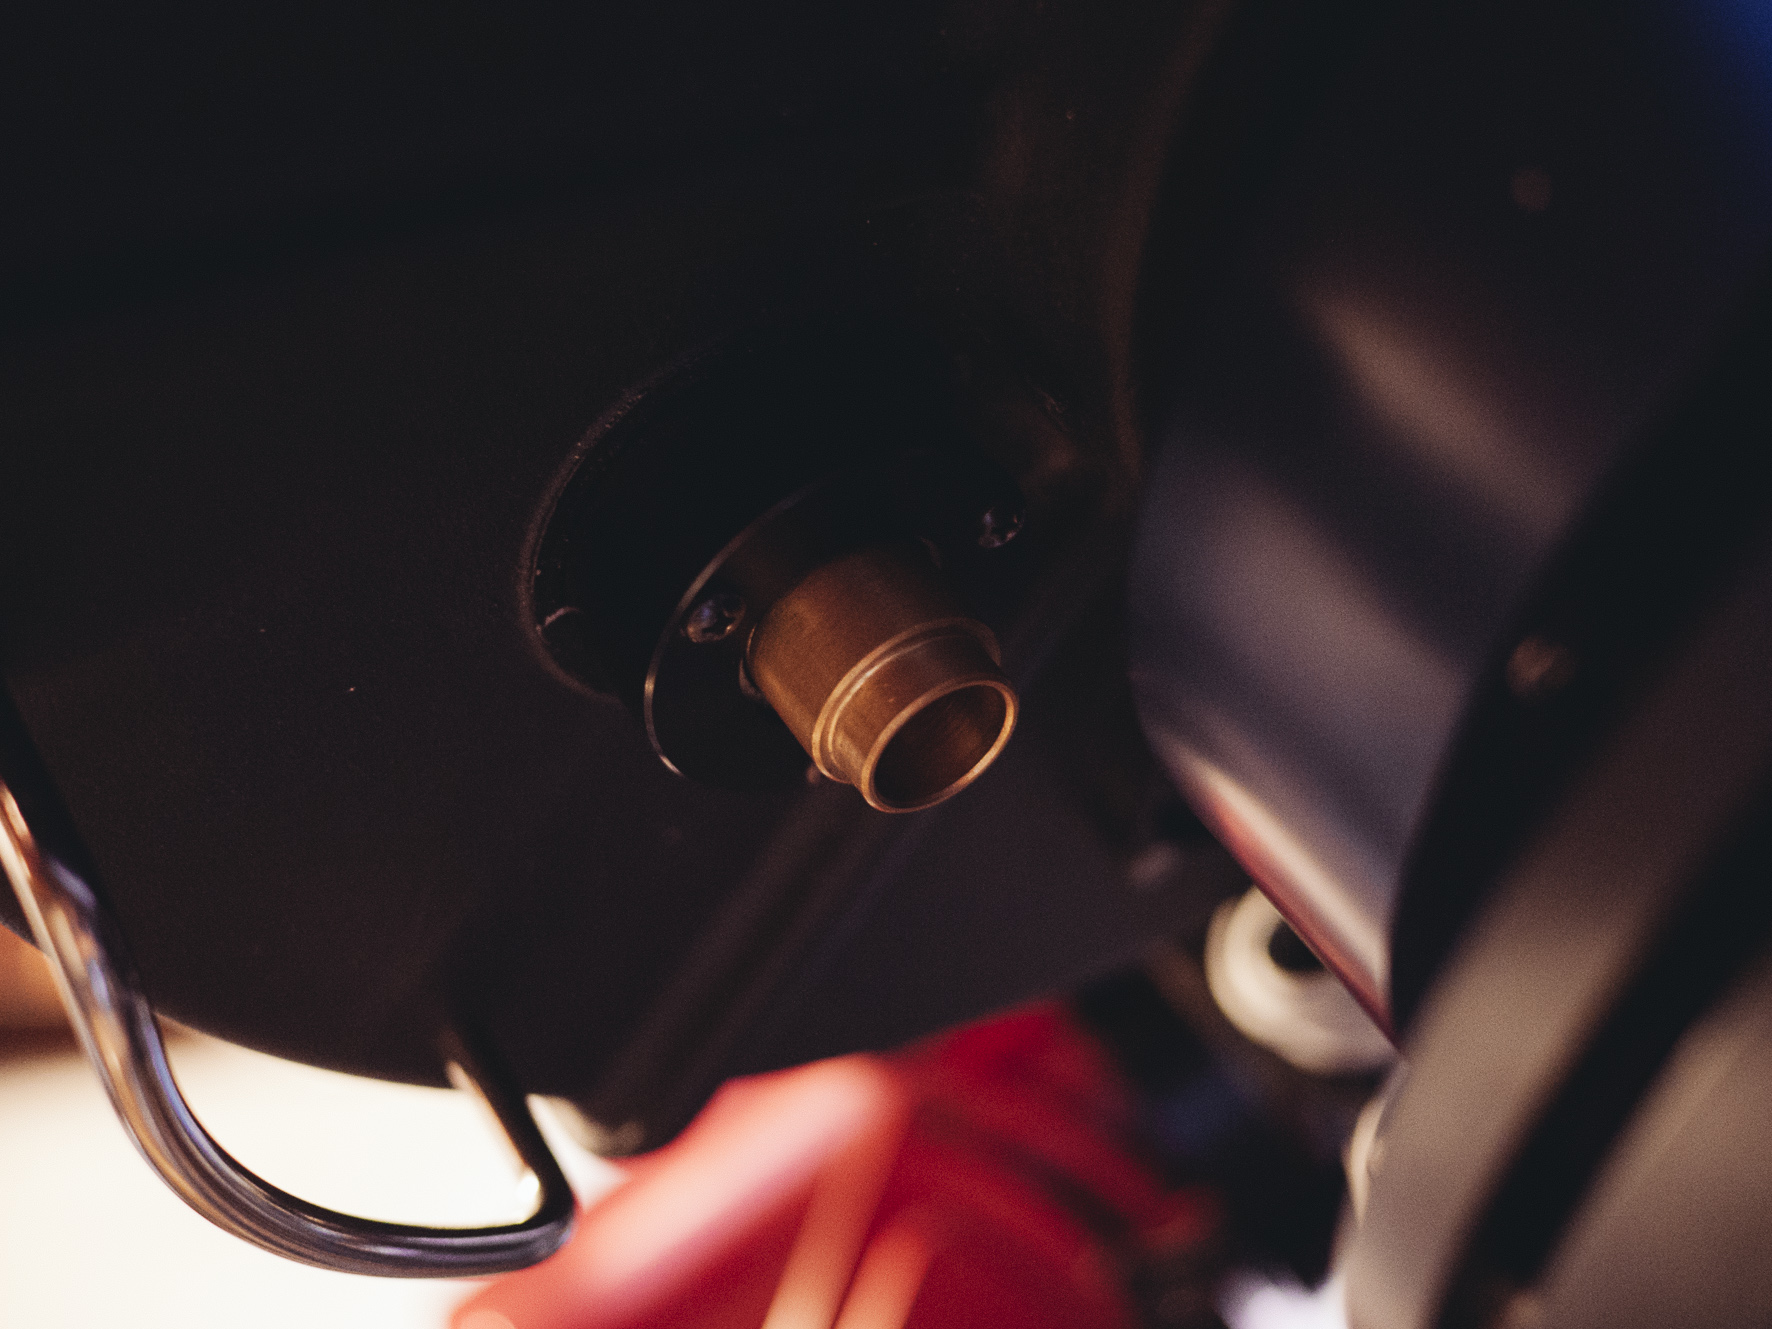
\includegraphics[width=0.75\textwidth]{documentation_images/focus_knob.jpg}
    \caption{\label{fig:focus_knob}The focus knob at the back of the telescope.}
 \end{figure}

 \item Depending on how out of focus the telescope is, you should now (after the initial image is taken) see an image with blurry dots or faint `donuts' which are very out of focus stars.
 \item Now you need to adjust the telescope's focus. Do this by turning the brass focussing knob at the back of the telescope (seen in Figure~\ref{fig:focus_knob}) in small increments either clockwise or anti-clockwise.
 \item If the focus gets better the stars in the continuously-updating image should get sharper. If they don't, try turning the focusing knob in the other direction. 
 \item Continue this process until the stars in your focussing image is as sharp as possible.
 \item For precise photometric measurements, you may want additional reassurance that the telescope is in focus. Clicking on the \textbf{Graphs} button will bring up a plot of x and y pixel positions on the CCD versus brightness. The better the focus, the narrower and the higher the brightness peak will be –- and the smaller the FWHM value of the peak. Adjust the focus until this the FWHM-value is as low as possible.
\end{enumerate}

\subsection{Selecting a guide star}
\begin{enumerate}
 \item Step 1
 \item Step 2
 \item Step 3
 \item Step 4
 \item Step 5: Got it!
\end{enumerate}


%\subsection{Remote Observations}
%\label{remote_obs}

%\subsection{Dome Control}
%\label{Dome_control}
%TBA
%\label{dome_position}

\vfill \eject 

\section{Science imaging}

\subsection{CCD Setup}

\subsection{Taking Images}
\label{taking_images}

\begin{enumerate}
 \item Individual images
 \item Exposing a sequence
\end{enumerate}

\subsection{Adjusting Images}

\subsection{Saving Images}

\clearpage

\subsection{Calibration Images}
\label{calibration}

Depending on the circumstances, it may be necessary to take a series of calibration images to correctly reduce your light frames. An existing library of calibration images exists on the {\tt darkstar} server at {\tt ftp://darkstar.ast.uct.ac.za/}. These may however not always be appropriate to correctly reduce your science images, and you may thus have to allow time during your observation to collect a new set. This section briefly describes the types of calibration images you may need, and how to take them.\\

Examples of typical calibration images from the telescope and CCD imager are shown in Figure~\ref{fig:cal}. These are hardly ever very interesting to look at, but makes a huge impact on the quality of your science images.\\

\paragraph{Bias Frames.}
  Bias frames are used to subtract the readout signal from the CCD itself, and amounts to basically a 0-second exposure. It is important that the bias frames are taken at the same CCD-temperature as the science frames you will be reducing them with. Bias frame exposures may be collected as part of a sequence of images while collecting light and dark images and are relatively straightforward to set up (see Section \ref{taking_images}). Between 10 and 20 bias frames are collected normally and then combined into a master bias frame later in the reduction pipeline.

\paragraph{Dark Frames.}
  Subtracting dark frames from your collected science images will correct for the accumulation of thermal, electronic and random noise on the CCD. The reason why the CCD is cooled is to reduce this noise as much as possible, but it can never be completely avoided. Dark frames account for this noise and is a time exposure (of the same duration as your light images) taken with the shutter closed. \emph{Maxim DL} and \emph{The SkyX} have built-in options to take dark frames either by themselves, or as part of a series.

\paragraph{Flat Fields.}
  Flat field images are taken to account for the large-scale variations in sensitivity across the CCD, caused by things such as the dust-specks on the lens or the telescope and instrument optics. Obtaining good flat field images is not easy and is usually done by median-combining multiple light images of the twilight sky or an evenly lit section of the inside of the dome. The final product is then used to divide out the pixel to pixel sensitivity in the science images.\\

\begin{figure}[ht]
  \centering
    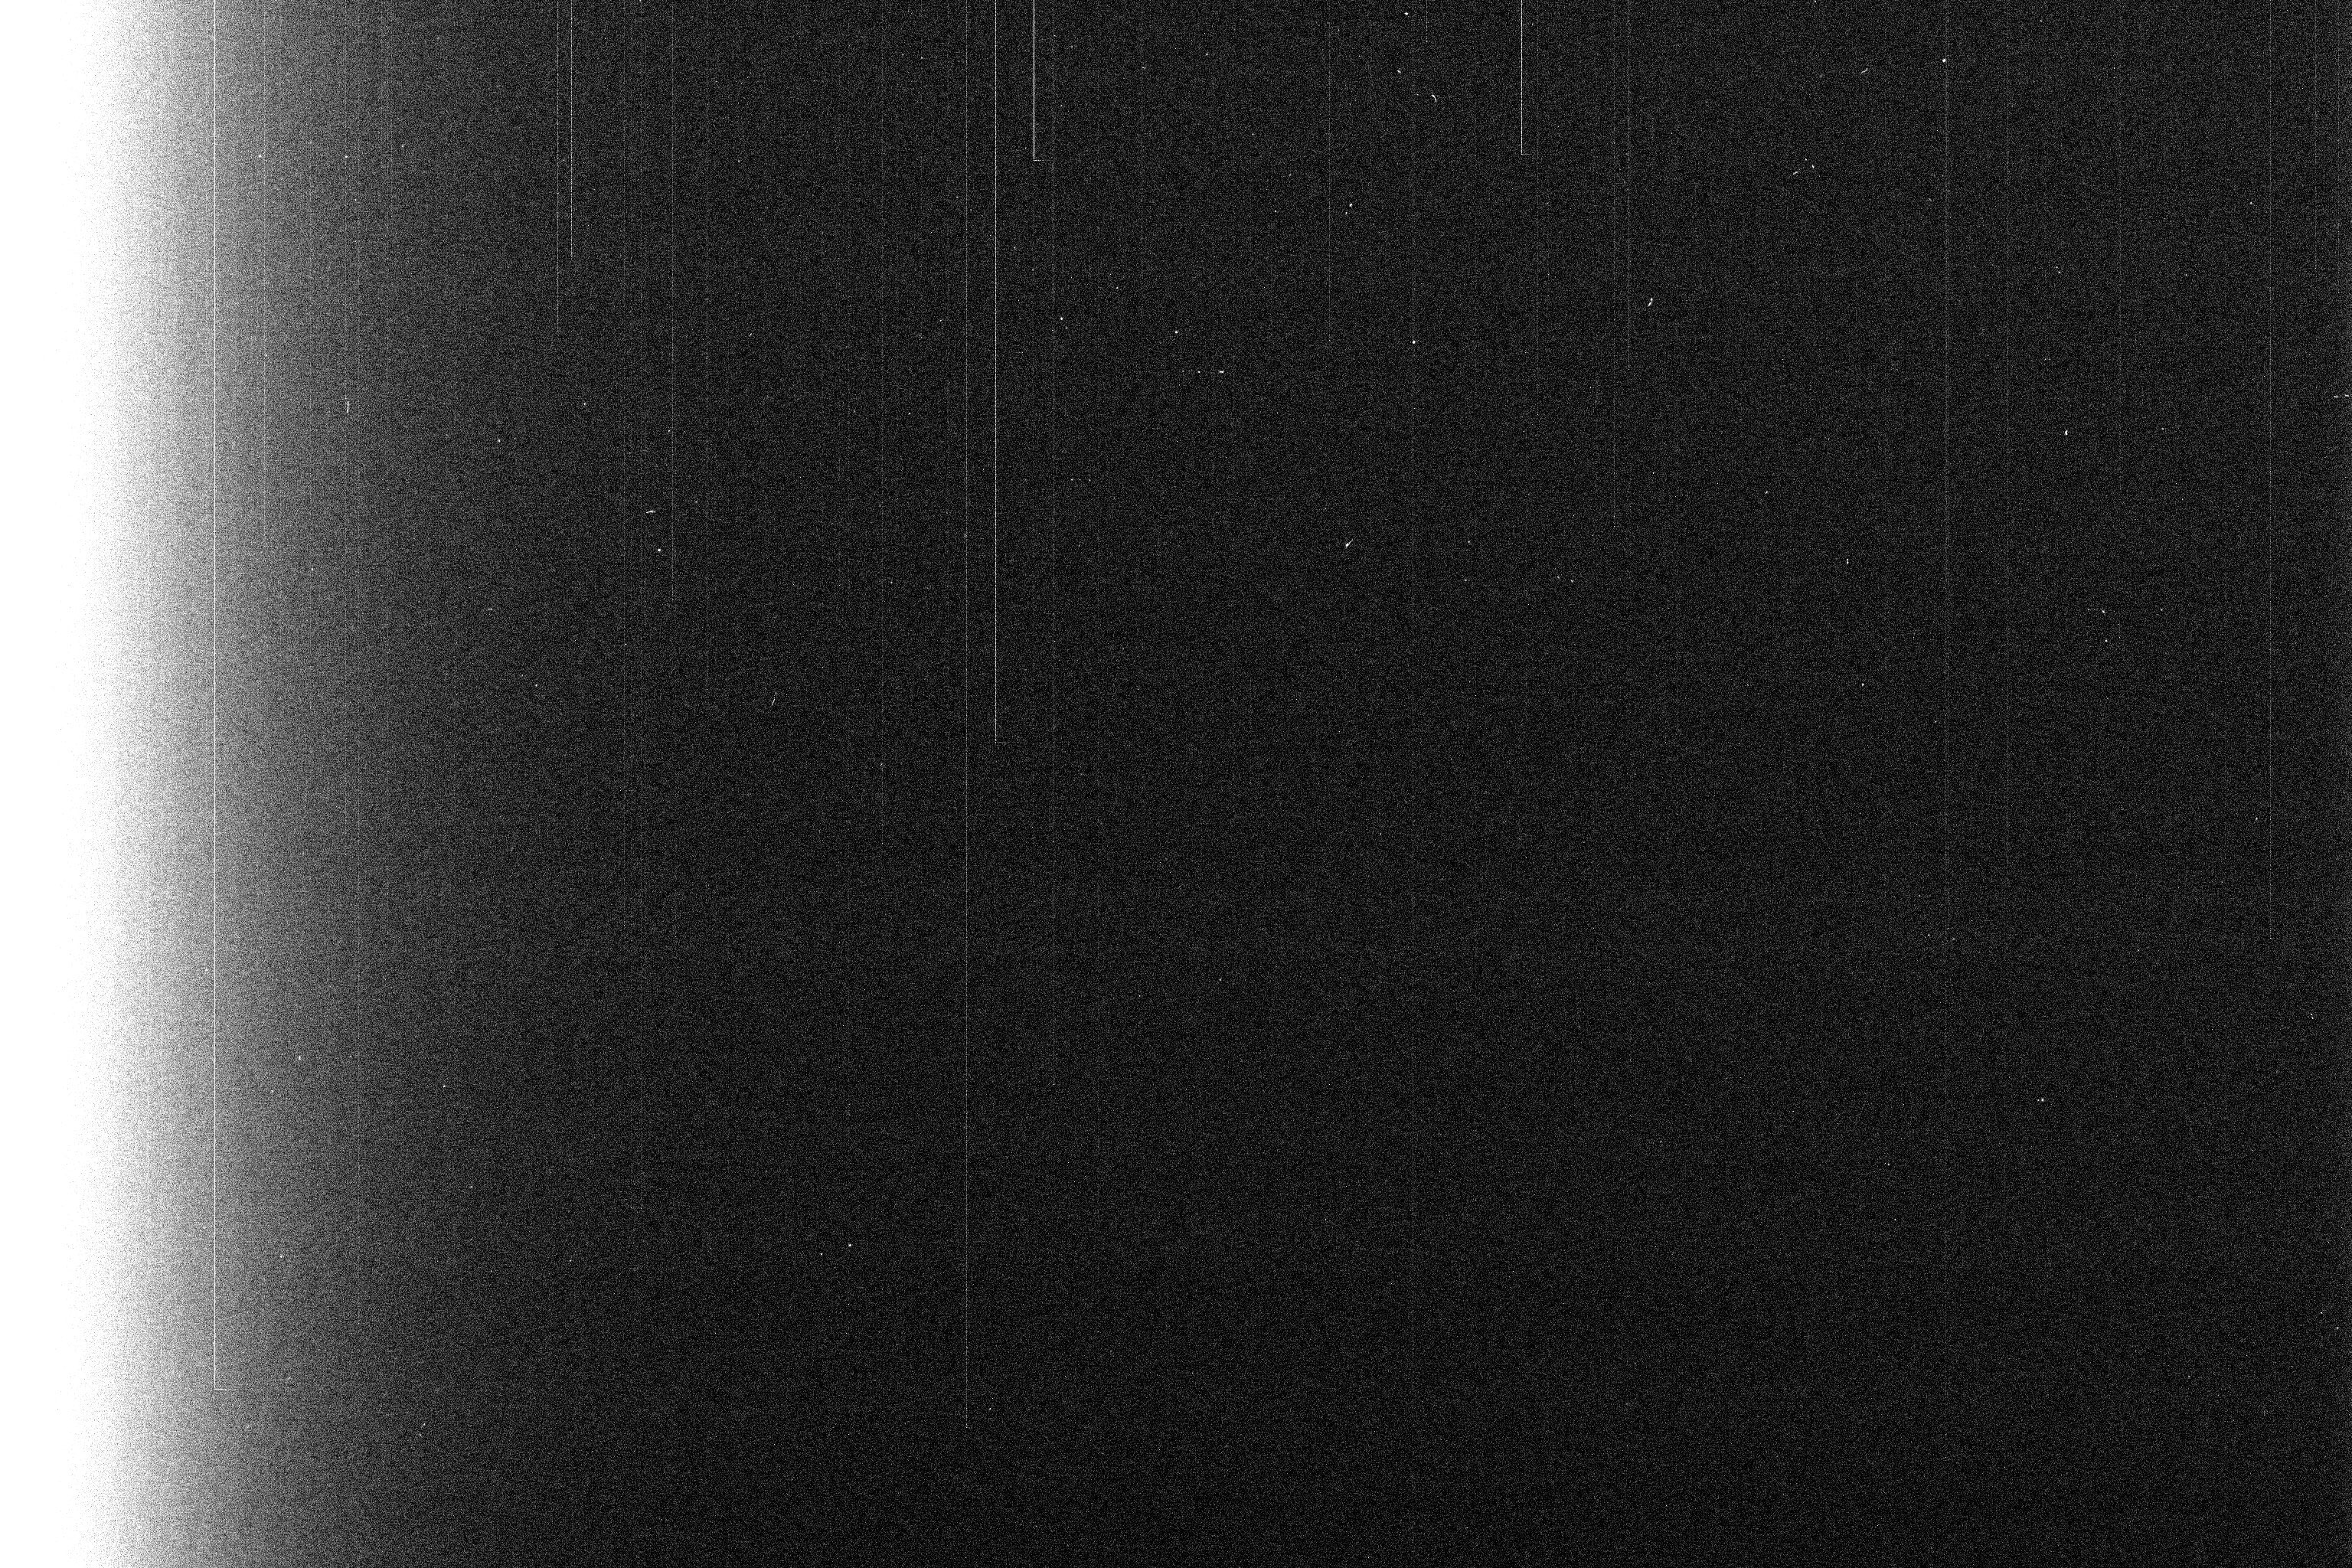
\includegraphics[width=0.32\textwidth]{documentation_images/calibration_bias.jpg}
    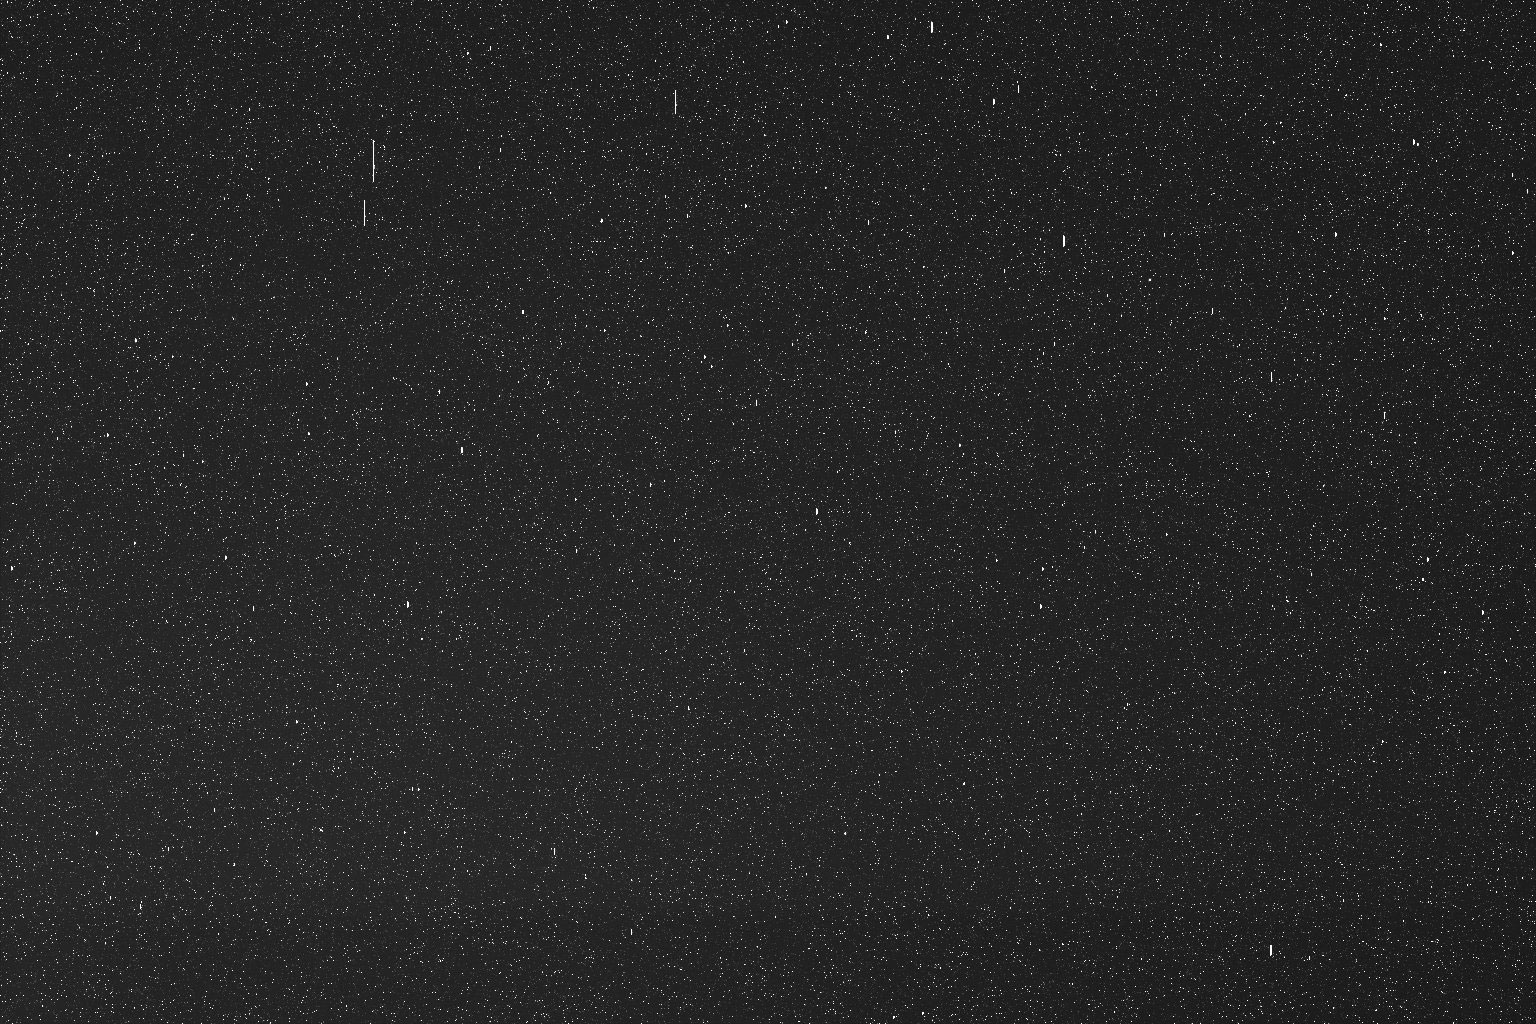
\includegraphics[width=0.32\textwidth]{documentation_images/calibration_dark.jpg}
    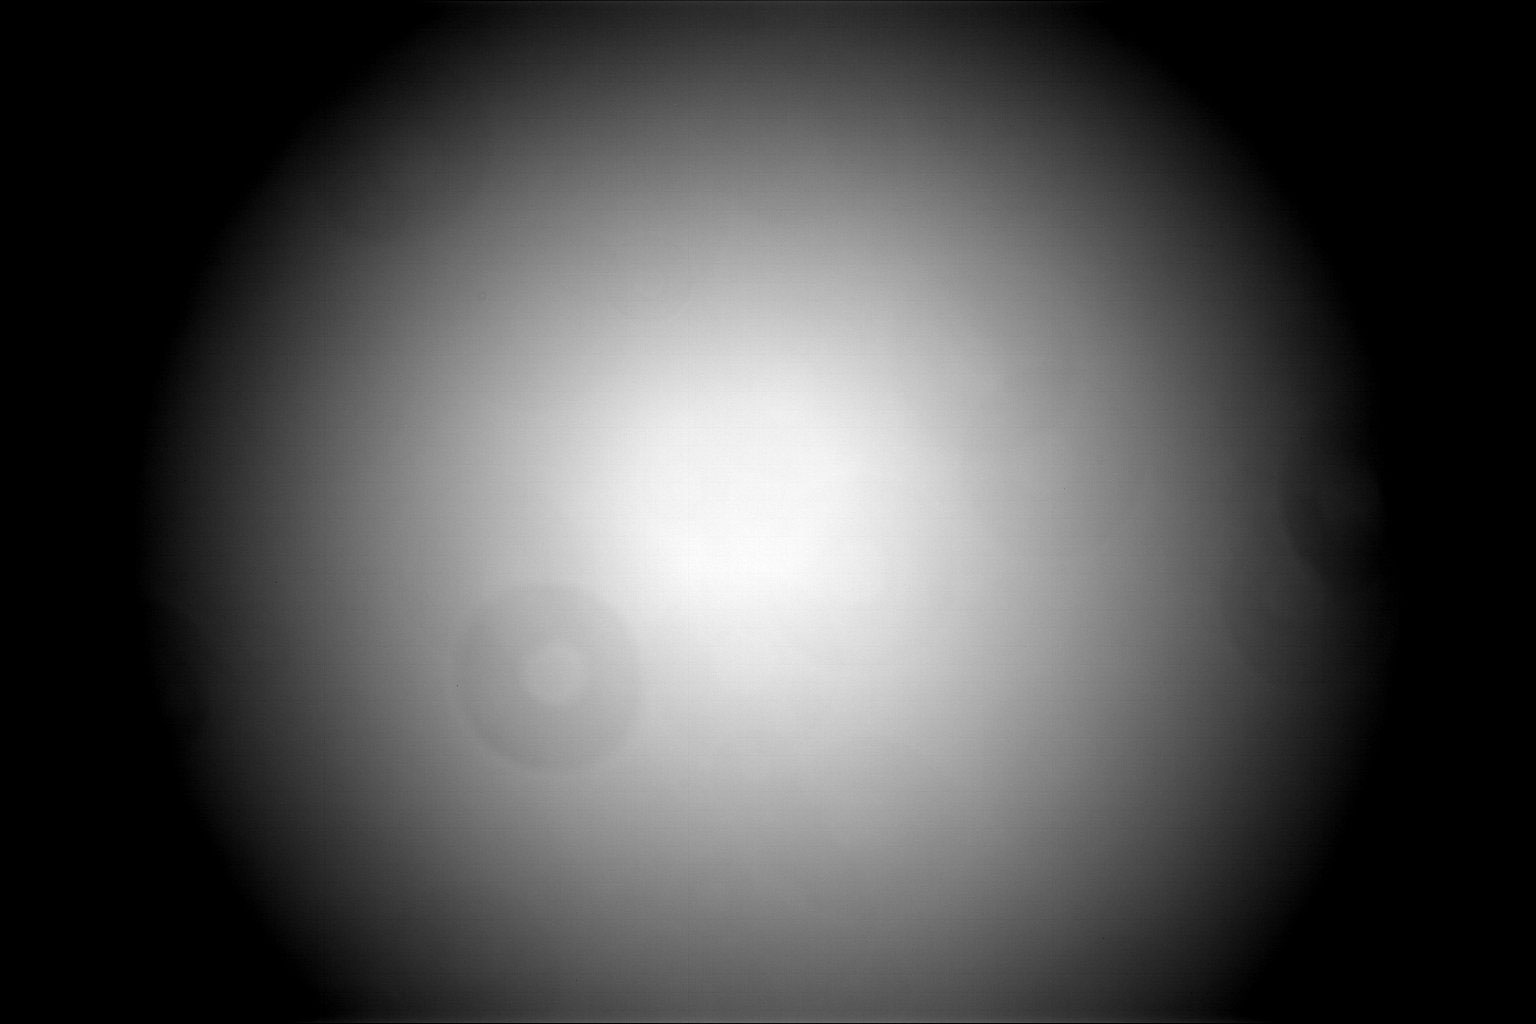
\includegraphics[width=0.32\textwidth]{documentation_images/calibration_flat.jpg}
    \caption{\label{fig:cal}Typical bias, dark and flat field calibration images.}
\end{figure}

\clearpage

\section{Close down procedures}

The close down procedure is the inverse of the start up process.\\

% \begin{enumerate}
%  \item In your CCD-controller, click on `Disconnect Camera'
%  \item In \emph{Maxim DL}, under the `Telescope' tab, click on `Park'. The telescope will slew into its parking position and sidereal tracking will be turned off. Once again, make sure the room is cleared from any objects (or persons!) the telescope might bump into.
%  \item Next you may click on `Disconnect Telescope'
%  \item In 'Dome' tab, click on `Park Dome'. Then, once the dome has come to a standstill in it's parking position, click on `Disconnect'.
%  \item You may now close the software, shut down the laptop and switch off all the wall plugs on the North and East walls
%  \item Set the RA and DEC drives on the telescope mount to their locked positions.
%  \item Replace the telescope's front cover and covering sheet.
%  \item Lastly, close the dome and make sure to set the closing latch in place.
% \end{enumerate}

\subsection{CCD control: \emph{Maxim DL}}

On the camera control window (\emph{Maxim DL}), click on `Warm Up' under `Coolers', and click `Disconnect' once camera 1
indicates that the cooler control is off.

\subsection{Telescope control: \emph{The SkyX}}

On \emph{The SkyX}, select the \textbf{Telescope} tab. Under the `Shut Down' pull-down menu, select \textbf{Park}, to 
slew the telescope to the park position (status should be green and read \textcolor{PineGreen}{\tt Parked}). 
Then select the \textbf{Dome} tab and select \textbf{Park Dome} to move the dome to the park position. Then select \textbf{Disconnect} (status should change to red and read \textcolor{BrickRed}{\tt Not Connected}).\\

Select the `Rotator' tab and select \textbf{Disconnect} (status should change to red and read \textcolor{BrickRed}{\tt Not Connected}).
Finally, under `Telescope', and the `Shut Down' menu, select \textbf{Disconnect} to disconnect the telescope (status
should change to red and read \textcolor{BrickRed}{\tt Not Connected}). The telescope is now parked.

\subsection{Locking the RA and DEC drives}

Change the RA and DEC drive clamps from the `star' position to the `locked' positions. 
Notice that the telescope will move a bit even when it is in the `locked' position. Move the
telescope until it physically locks into the `locked' position.

\subsection{Pull test and covers}
Recheck that the CCD is attached with a quick pull test. When you are satisfied that the instruments are safe, replace the telescope's front cover and covering sheet. Ensure that the front cover sits in place properly and that the sheet is draped so as to cover both the telescope and the instrument stack.

\subsection{Disconnect power}

Save any unsaved open files on the laptop on the hard drive or server, close any open applications, then shut down the laptop and close the lid. After that you may switch off all the wall plugs on North and East walls of the room.

\subsection{Close the dome}

Finally, you'll need to once again apply some elbow grease to close the dome. With the shutters closed, flip over the locking latch (Figure~\ref{fig:latch}) on the bottom of the left shutter to ensure that the dome stays closed. The observatory is now shut down and you are ready to leave. Before leaving, make doubly sure to have the keys to the observatory \emph{in you hand!} It is deceptively easy to lock the keys inside the room.\\

\begin{figure}[ht]
  \centering
    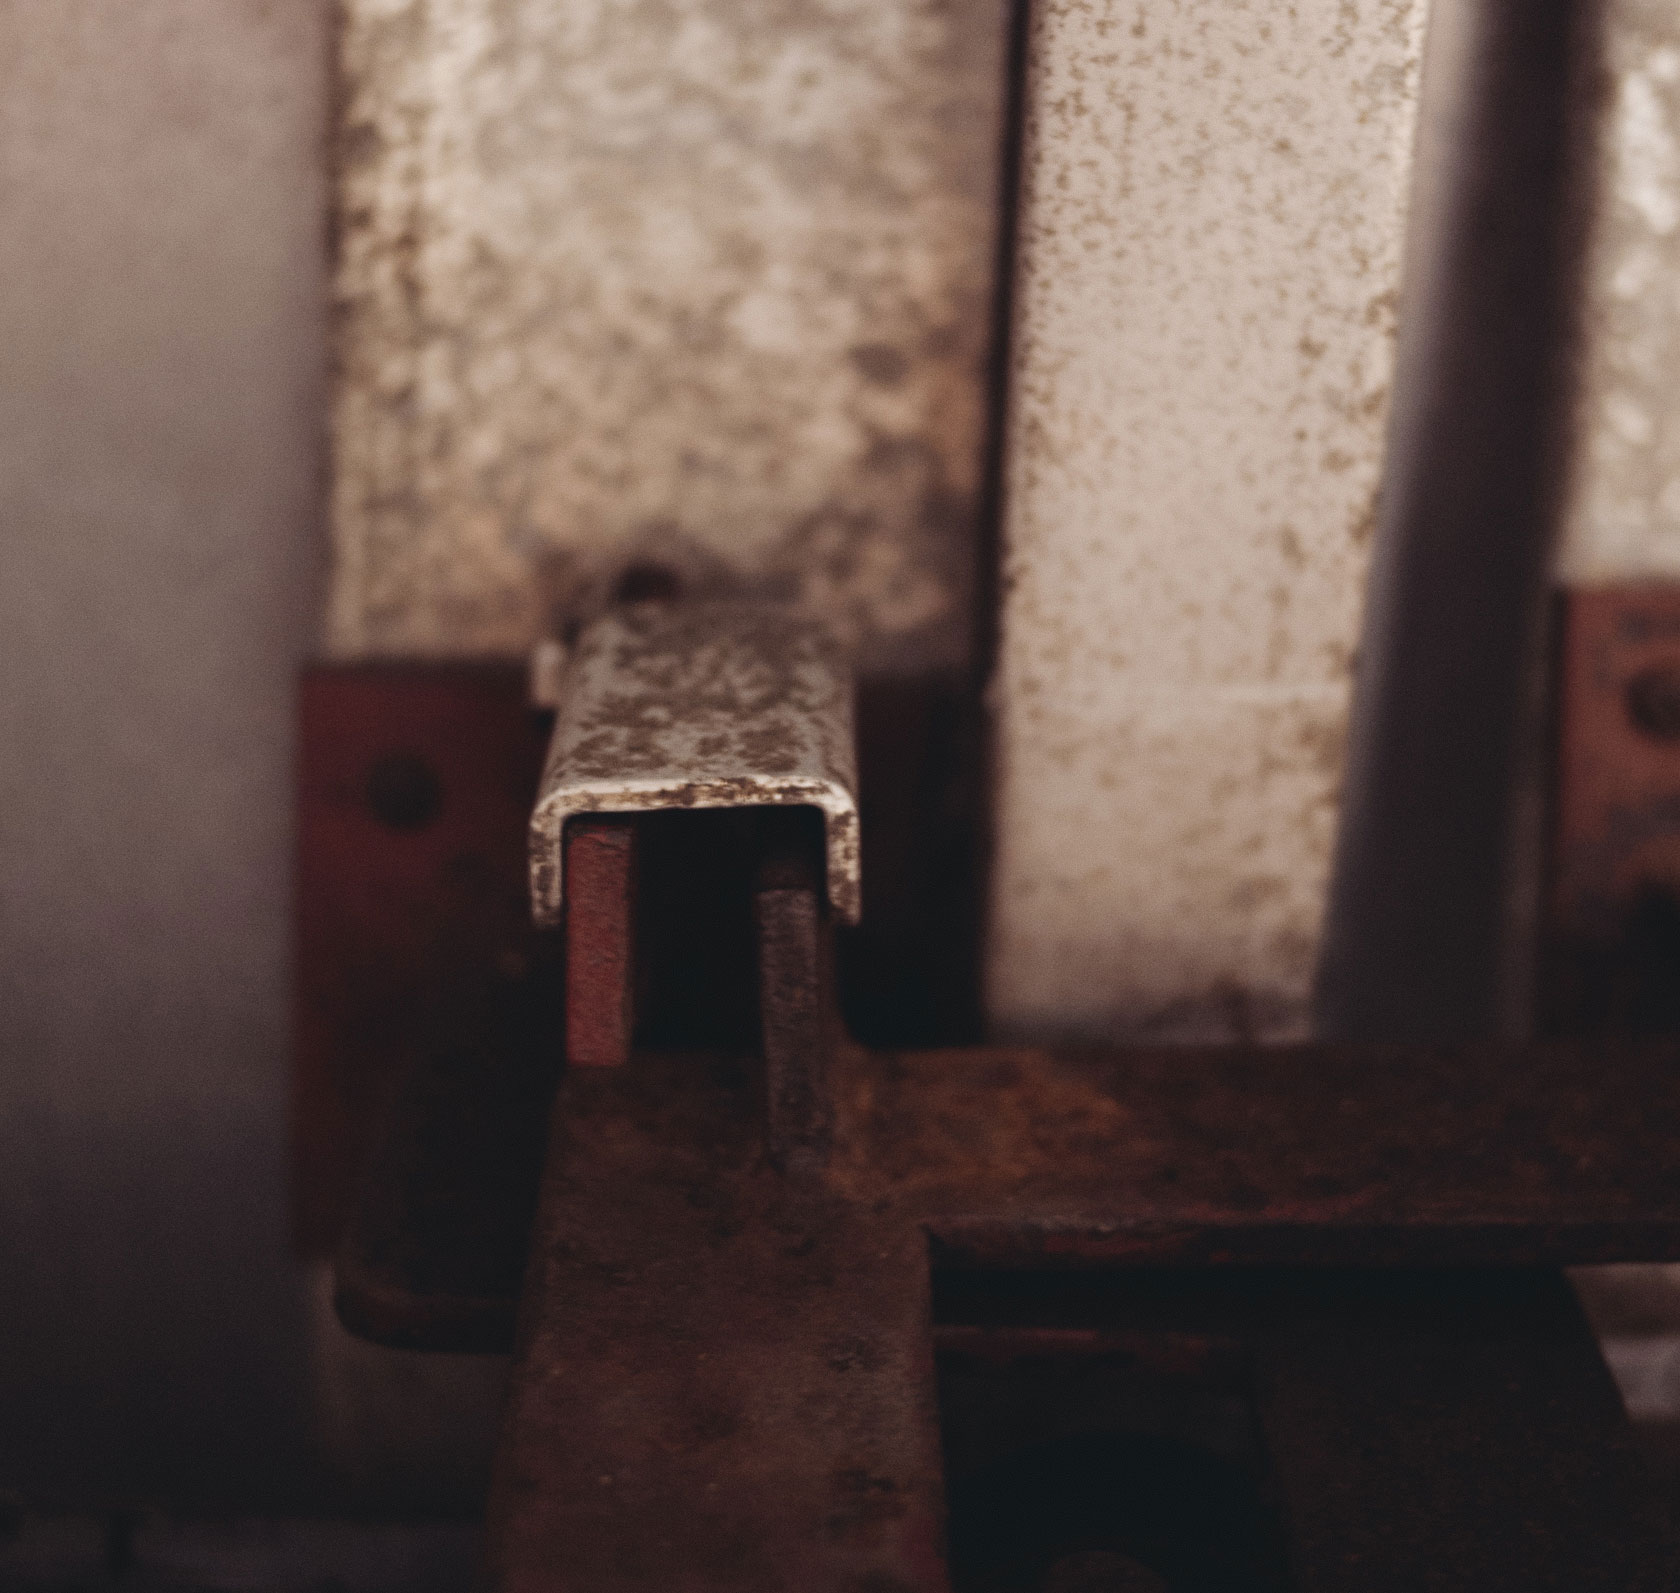
\includegraphics[width=0.5\textwidth]{documentation_images/domelatch.jpg}
    \caption{\label{fig:latch}Latch in place to keep the dome securely closed}
\end{figure}

%\clearpage

\section{In the event of a power failure}

Should the power go off during an observation session, the uninterrupted power supply (UPS) will continue to supply power to the telescope, laptop and instruments until it has no more battery life left.\\

If the power remains off for more than a couple of minutes, it may be a good idea to call it a night and get some well-deserved sleep. Follow the close down procedures as described earlier to shut down the telescope and the dome safely before you leave.\\

\clearpage

\section{Important phone numbers and observer safety}

It's is very important, no matter how absorbed you might be in the night sky, to always be vigilant and safe. Try to always observe in groups rather than alone -- an extra pair of eyes is always a good idea, plus you'll have someone to take over the frequent coffee-making duties (if you ask nicely).\\ 

For technical troubles or difficulties with the software, telescope or dome, the first person to contact is Thuso Simon on \textbf{073 535 2201}. For any non-urgent queries you may also email him at {\tt thuso.simon@gmail.com}.\\

UCT has it's own 24/7 Campus Protection Service. On upper campus, they are based in the Robert Leslie Social Sciences Building. CPS will gladly escort you back to your residence on lower campus, or wait with you for other transport to arrive.\\

Some important numbers to keep handy:

\renewcommand{\labelitemi}{$\bullet$}
\begin{itemize}
 \item Campus Protection Services: \textbf{021 650 2222/3}
 \item All emergency services (police, fire brigade, ambulance and sea rescue) can be accessed from you your cellphone by dialling \textbf{112}.
 %If you need sea rescue services while observing at UCT you are doing something very wrong.
 \item City of Cape Town fire \& rescue: \textbf{107} from a landline, or \textbf{021 480 7777} from a cellphone.
 \item SAPS (Rondebosch): \textbf{021 685 4747}
 \item SAPS (Mowbray): \textbf{021 680 9580}
 \item SAPS (Woodstock): \textbf{021 442 3122}
\end{itemize}

There are many private taxi services available if you need to get home in the the small hours of the morning. It's advisable to give these a call about an hour before you want to leave. Among the more reputable companies are:
\begin{itemize}
 \item Cabco: 086 136 7222 or 021 671 3836
 \item Excite: 021 448 4444
 \item Rikkis Taxi: 0861 745 547 or 021 447 3559
\end{itemize} 

\clearpage

\section{Check lists}
\label{checklists}

%If you want to get started at making images quickly and don't have the time to get into the nitty gritty details of astronomy 
%go to the next section.

\subsection{Start of Night Check List}

\begin{enumerate}
 \item Check the weather!
 \item Plug observation computer into power \& internet, then dome controller and telescope controller USB cables into the laptop. Turn on switches in the observatory.
 \item Open the dome and take off the telescope cover.
 \item Do a pull test on the instrument stack.
 \item Put the telescope mount from `lock' to `star' position on both RA and Dec controllers.
 \item Start \emph{TheSkyX} and \emph{Maxim DL} on the laptop.
 \item Connect observation computer to internet if wanting to use remote software (see \ref{remote_obs} for more information). 
 \item Make sure no chairs, tables or other objects are in the way of telescope's movement.
 \item Connect dome control, rotation and mount control in \emph{TheSkyX}. Tell all to go to home position and start! 
See section \ref{telescope_control} for more information.
 \item Find star to focus (less than 7.5 - 9 magnitude star) using Focus Max.
  \item Fine tune dome position (see section \ref{telescope_control}).
 \item Slew to object, select filter, check rotation; then expose and get some coffee.
\end{enumerate}

\vspace{1.0cm}
%coffee stain
%\cofeAm{.1}{1.0}{0}{5.5cm}{3cm}


\subsection{End of Night Check List}

\begin{enumerate}
 \item Park telescope and Dome and disconnect all systems from computer.
 \item Turn off observation computer.
 \item Put RA and DEC drives from star position to lock position.
 \item Power off all power supplies in dome.
 \item Close the dome shutter.

 \item Replace telescope lid and cover the telescope.
 \item Get some sleep.
\end{enumerate}



%--------------------------------
% Photometry
%--------------------------------

\chapter{Photometry}

Photometry is concerned with measuring the brightness of an object. Whether that object be a star, a planet, an asteroid or a galaxy, photometric measurements can give a valuable insight into it's behaviour and characteristics. Doing photometry on a time-series can in addition give you information on how these properties change over time or reveal details about the object's environment.\\



\section{Getting WCS coordinates in your image}

There are several bits of information necessary to do accurate photometric measurements, some of which can be written as meta data into the header of the {\tt .FITS} files (images) you will take. Among these are things like the filter used and exposure time, but, very importantly, you will also need the correct WCS (world coordinate systems) coordinates. From the WCS coordinates it is possible to not only to correctly identify your object, but also compute the \emph{airmass} -- the optical path length through the atmosphere through which your object is observed. The airmass information will be used when doing magnitude calculations later.\\

\subsection{With \emph{MaximDL}}
When taking an image with \emph{MaximDL}, the software already writes approximate RA and DEC values to the {\tt .FITS} header. \emph{Maxim DL} has built-in functionality to perform more accurate astrometry on an image you take, and if the astrometric analysis is successful, add WCS coordinates to the {\tt .FITS} file header. To access this tool, which uses the PinPoint astrometric engine, go to \emph{Analyse –- PinPoint Astrometry}. The various settings should already be set up correctly and the image parameters pulled in from the existing {\tt .FITS} header. Click on \textbf{Process} to begin solving your image.\\

\subsection{With {\tt astrometry.net}}
Should your solve be unsuccessful and fiddling with the setting not get you anywhere, you may want to try uploading your {\tt .FITS} image to {\tt http://astrometry.net/}. This is a fantastic free tool that can solve some very tricky images and provide you with a host of information about your image. Note that if {\tt http://astrometry.net/} solves your image and provides you with astrometric data, you will manually need to add the data back to the {\tt .FITS} header of your image(s) using a suitable {\tt .FITS} header editor.\\

See Section~\ref{autoapi} on the automatic reduction API to see how to automatically upload and solve your images as part of the image reduction pipeline.

\subsection{With \emph{The SkyX}}
Using the \emph{Image Link} functionality in \emph{The SkyX}, as described in section \ref{pointing} will also get you correct WCS coordinates. After linking an image successfully, the \emph{`Astrometry'} and \emph{`Cursor Information'} windows will give you detailed information about the objects in the image, including precise position. The {\tt .FITS} header will in this case have to be updated manually too.\\

The \emph{`Cursor Information'} window also gives you the \textbf{scale} of your image. If you failed to find an astrometric solution in \emph{Maxim DL} earlier, it could have been that the image scale was set wrongly and you might now want to use this information to try again.



\section{Standard Stars and Calibration}

One of the most important steps in doing accurate CCD photometry is calibrating, or reducing, your image properly. For this you would need the usual set of \textbf{bias, dark} and \textbf{flat field} images (see Section~\ref{calibration}), to correct for any unwanted noise. Suitable calibration images matching the current imaging conditions and parameters (CCD temperature, exposure time, filter used, etc) might already be stored in the calibration image library on the {\tt darkstar} server. If not, you would need to allow time during your observation run to collect these too.\\

When doing differential photometry, you will need calibrated data on the standard or reference stars in your FOV (or as close by in the sky as possible). The Variable Star Plotter (VSP) is a tool to generate a plot of reference stars from the latest data in the Variable Star Index. The VSP is available at {\tt http://www.aavso.org/standard-stars-vsp}.



\section{Aperture photometry}

Aperture photometry in it's simplest form, is a way to take photometric measurements from a point source, by adding up pixel counts in a circle centred on the object and subtracting the light due to the sky. \\

% \[object flux = total counts - sky counts]

Measurements for your target and the background sky can be taken simultaneously with a multiple aperture instrument, or, in the case of CCD detectors, by using software to select apertures for the target and the sky. Usually a round aperture is centred on the object, with a larger annular ring just outside to measure the sky. An additional `gap' may also be specified through which you can select any object to specifically exclude from your measurements. An example of such a setup is shown below in Figure~\ref{fig:annulus}.\\

For a brief guide on how to do aperture photometry in AstroImageJ, see Section~\ref{AIJ_Photometry}.

 \begin{figure}[ht]
  \centering
    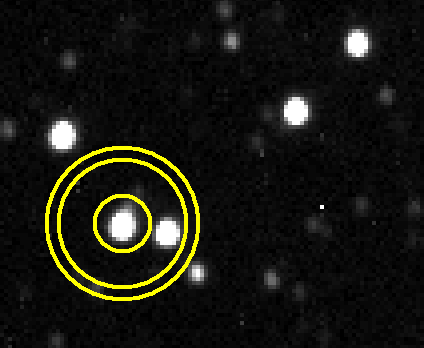
\includegraphics[width=0.75\textwidth]{documentation_images/annulus.png}
    \caption{\label{fig:annulus}Aperture, gap and annuls}
 \end{figure}

\section{The Point Spread Function}

Aperture photometry on crowded star fields, such as globular- or open clusters, will not generally give accurate results. In this case it is better to make use of a Point Spread Function -- a Gaussian that can be fitted to all the stars in your field in order to find their magnitude.

%from wikipedia: "When doing photometry in a very crowded field, such as a globular cluster, where the profiles of stars overlap significantly, one must use de-convolution techniques, such as point spread function (PSF) fitting, to determine the individual fluxes of the overlapping sources.""

\section{Photometric filters}

\section{Differential photmetry}

%Comparison to standard stars in same FOV? (via AAVASO catalogue)



%--------------------------------
% Spectroscopy
%--------------------------------

\chapter{Spectroscopy}

Detailed operating instructions for the SBIG Self Guided Spectrograph are also available from ${\tt www.sbig.com/site/assets/files/18237/sgs\_manual3.pdf‎}$.

\section{Positioning an object on the slit}

When attempting to collect the spectrum of an object, it is first necessary to point the telescope so that the object appears on the camera's tracking CCD. For the purposes of using the spectrograph, you can use \emph{The SkyX} to both position the telescope and control the CCD.\\

To correctly place an object to be analyzed you should do the following:\\

\begin{enumerate}
 \item Slew to the object you would like to investigate.
 \item In the `Autoguider' tab on the left side of the screen, set up and take a short exposure and make sure the object you selected appears on the resulting image. Adjust the telescope's pointing if needed. (Note: There's no need to save this, or any of the autoguiding images)
 \item Flip the switch on the bottom of the spectrograph (Figure~\ref{fig:internal_LED}, to turn on the internal LED. The LED back-lights the slit, which allows you to see it clearly when positioning your object.

 \begin{figure}[ht]
  \centering
    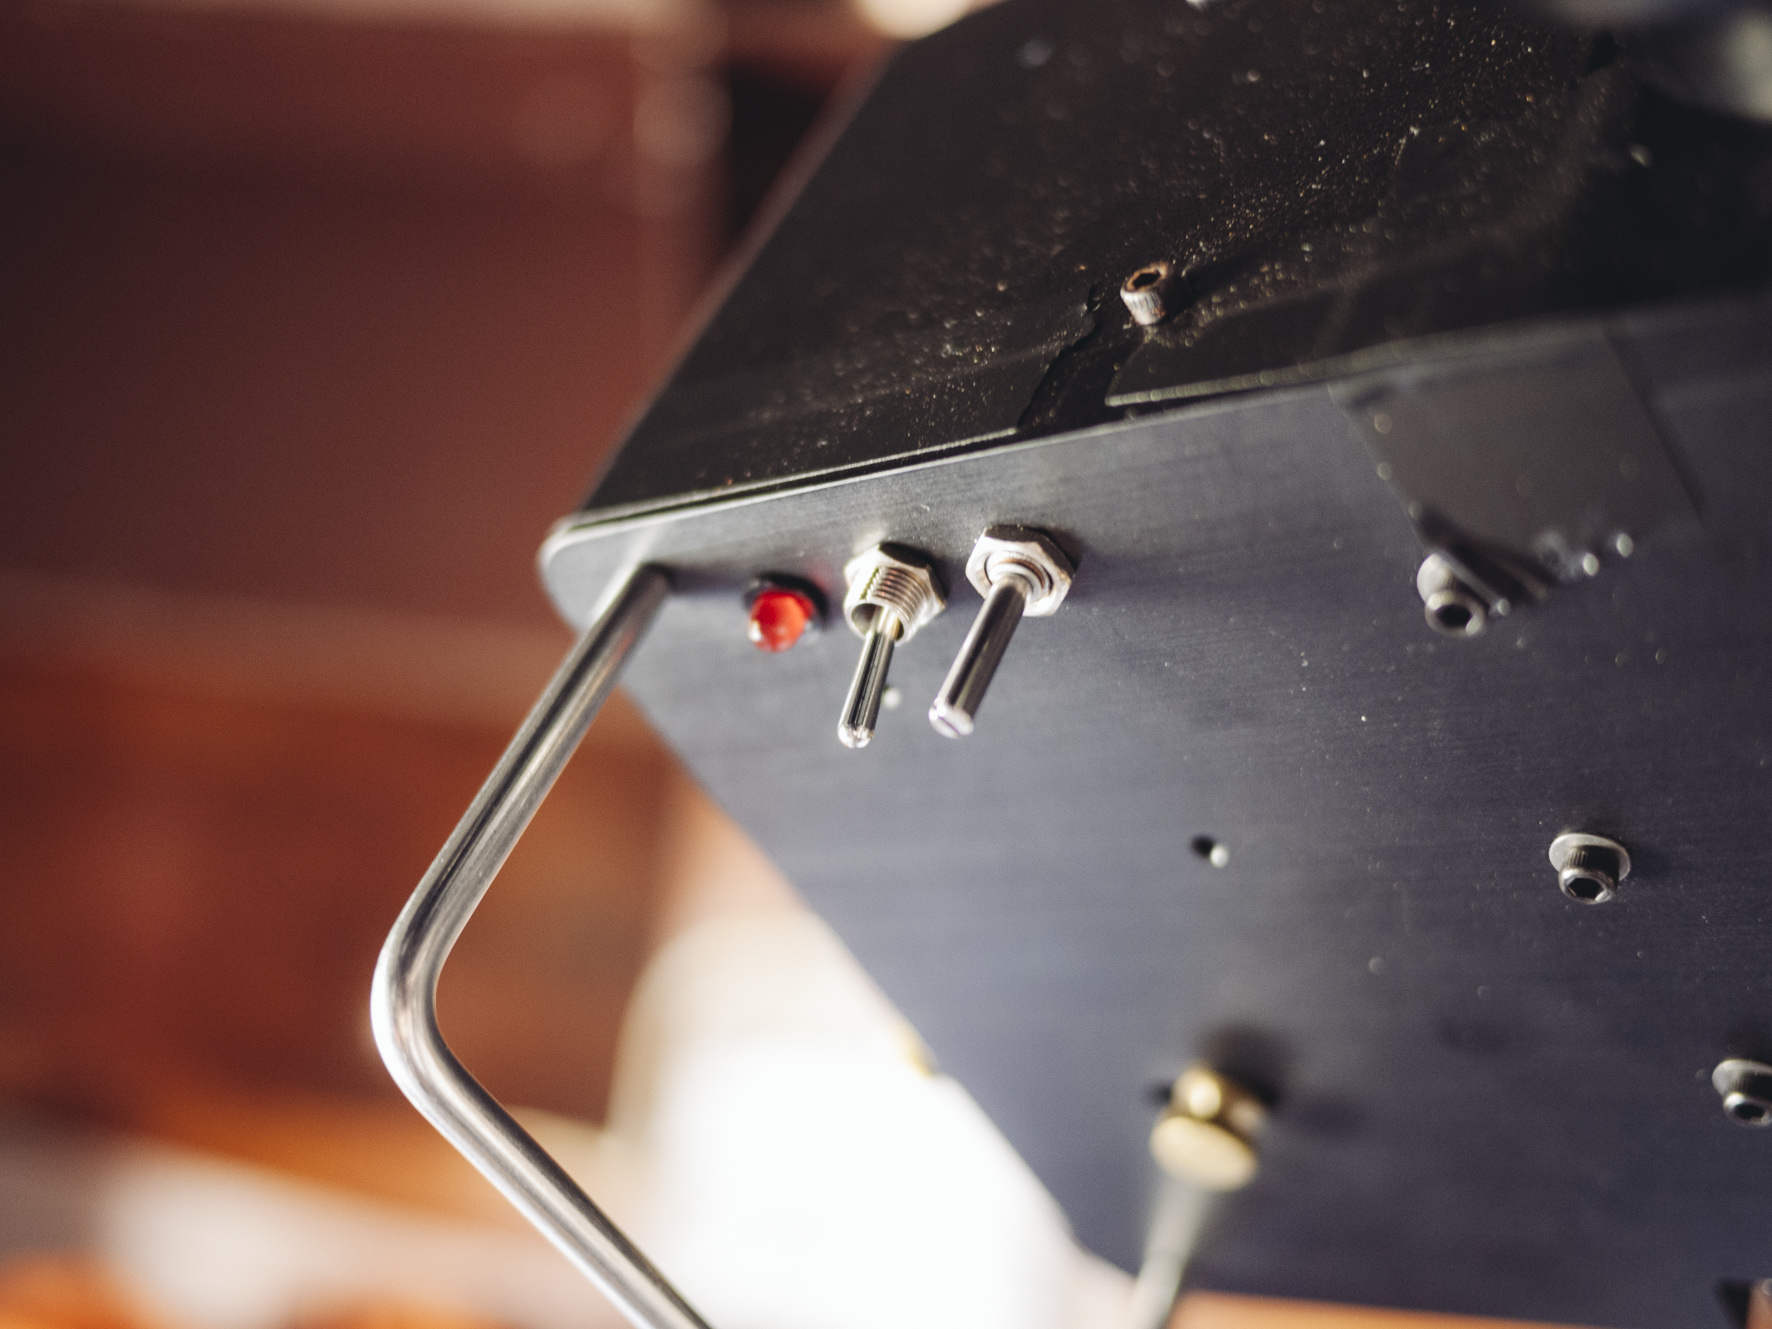
\includegraphics[width=0.49\textwidth]{documentation_images/internal_LED.jpg}
    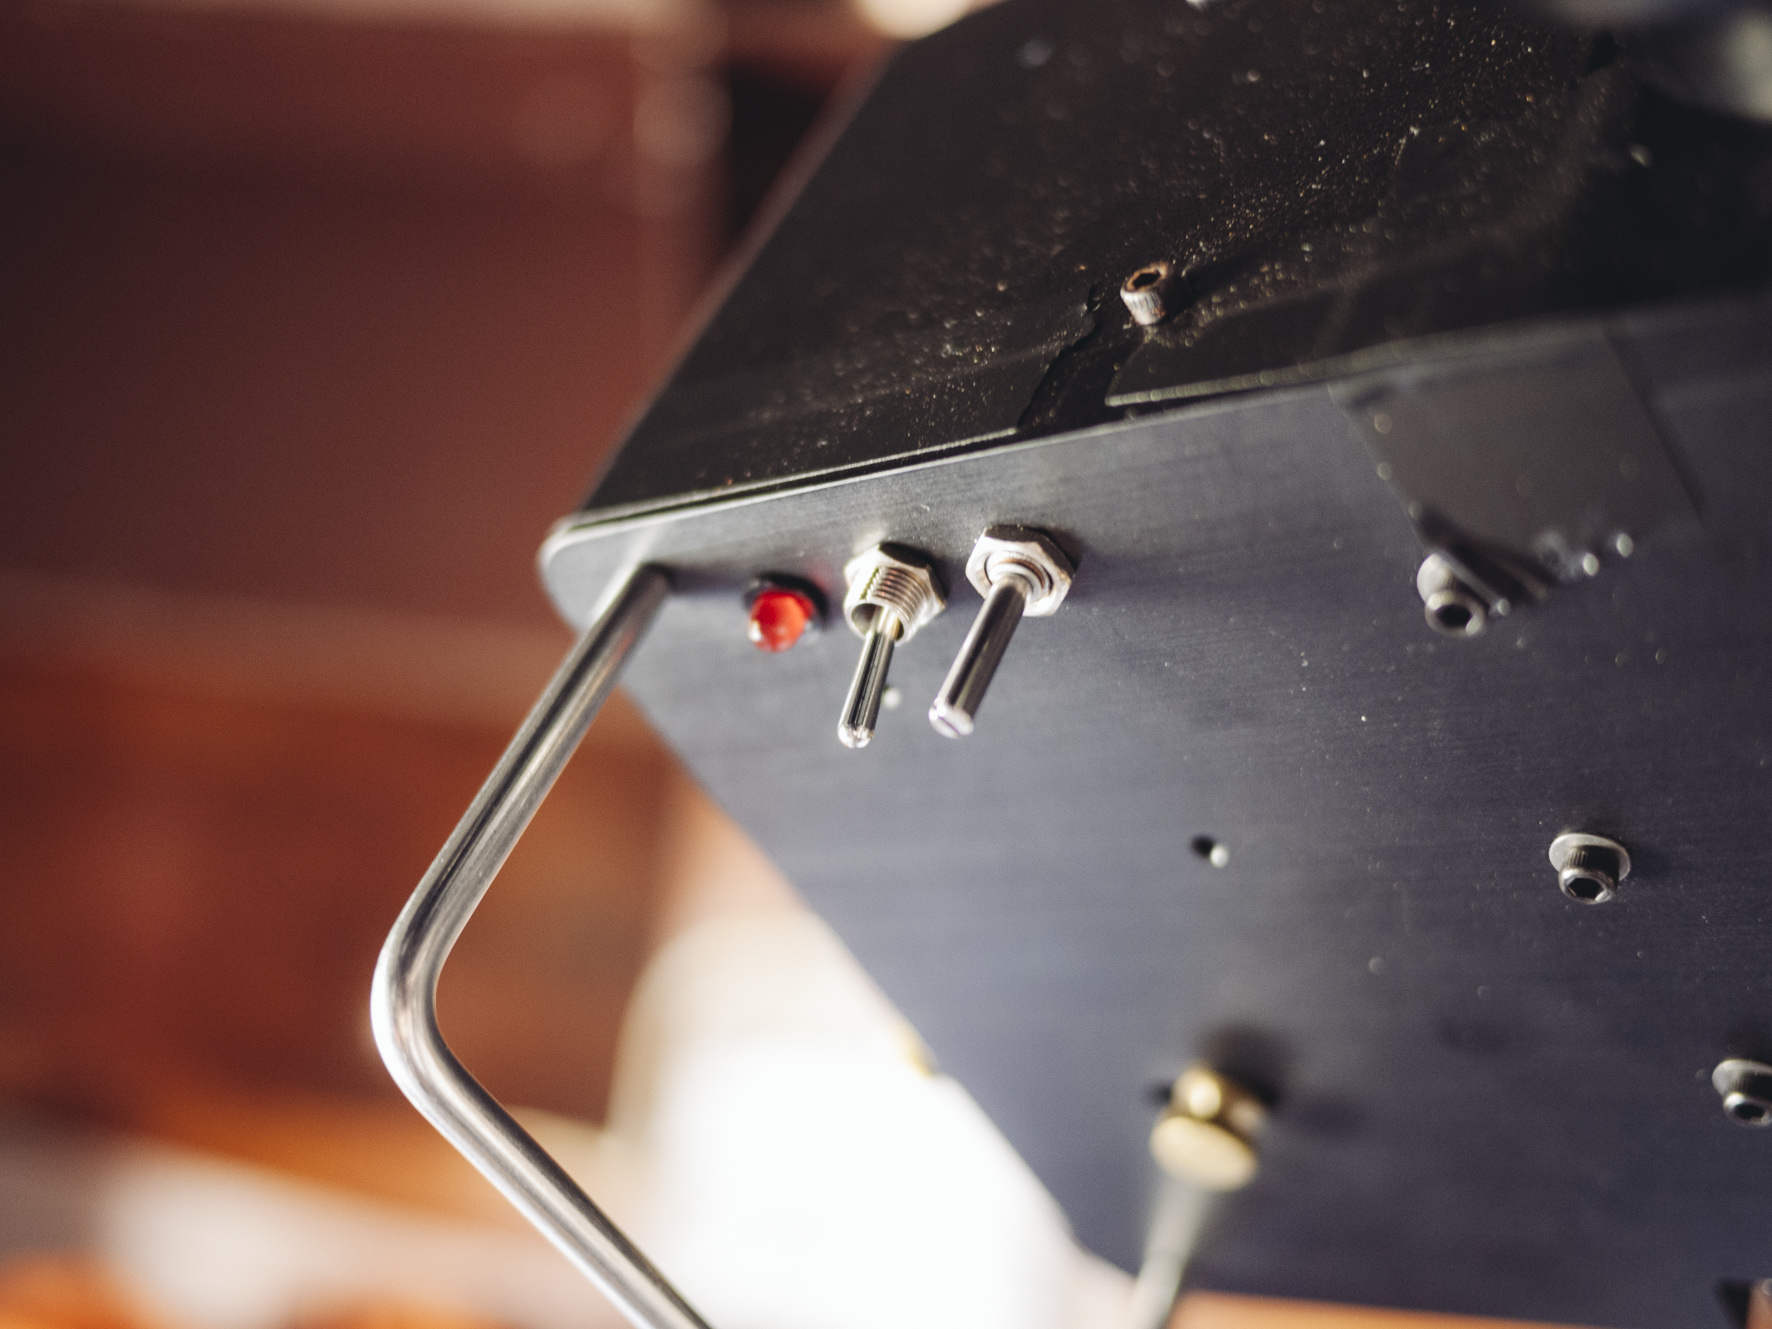
\includegraphics[width=0.49\textwidth]{documentation_images/internal_LED.jpg}
    \caption{\label{fig:internal_LED}LED switch on the spectrograph and the slit visible on the autoguide image. (R-image to be swooped out)}
 \end{figure}

 \item Still inside the `Autoguiding' tab, set up a continuous series of exposures, similar to the way you would when focusing the telescope (see section \ref{focussing}) then adjust the telescope so that your object falls right on the slit. You can adjust the telescope either with the hand-controller or with the green Up/Down/Left/Right arrows in the `Telescope' tab.

 \item If your object is a star, it is positioned correctly when it slightly straddles the slit. For extended objects, have the slit cut through the section you would like to take spectra from. Once you are satisfied with your alignment you may `Abort' the continuous exposures.\\

\end{enumerate}

Note that a bright star right on the slit might cause multiple images to appear, displaced horizontally. It should still be quite clear which one is the brightest, and therefore the actual star. If you are unsure, broaden the dynamic range of the displayed image until it is clear which object is the brightest.


\section{Set up Autoguiding}

To keep your object positioned on the slit as accurately as possible, you now need to activate the autoguiding feature.

\begin{enumerate}
 \item In the `Autoguide' tab, collect a new image (or if your last image is only a few seconds old, use that one)

  \begin{figure}[ht]
  \centering
    %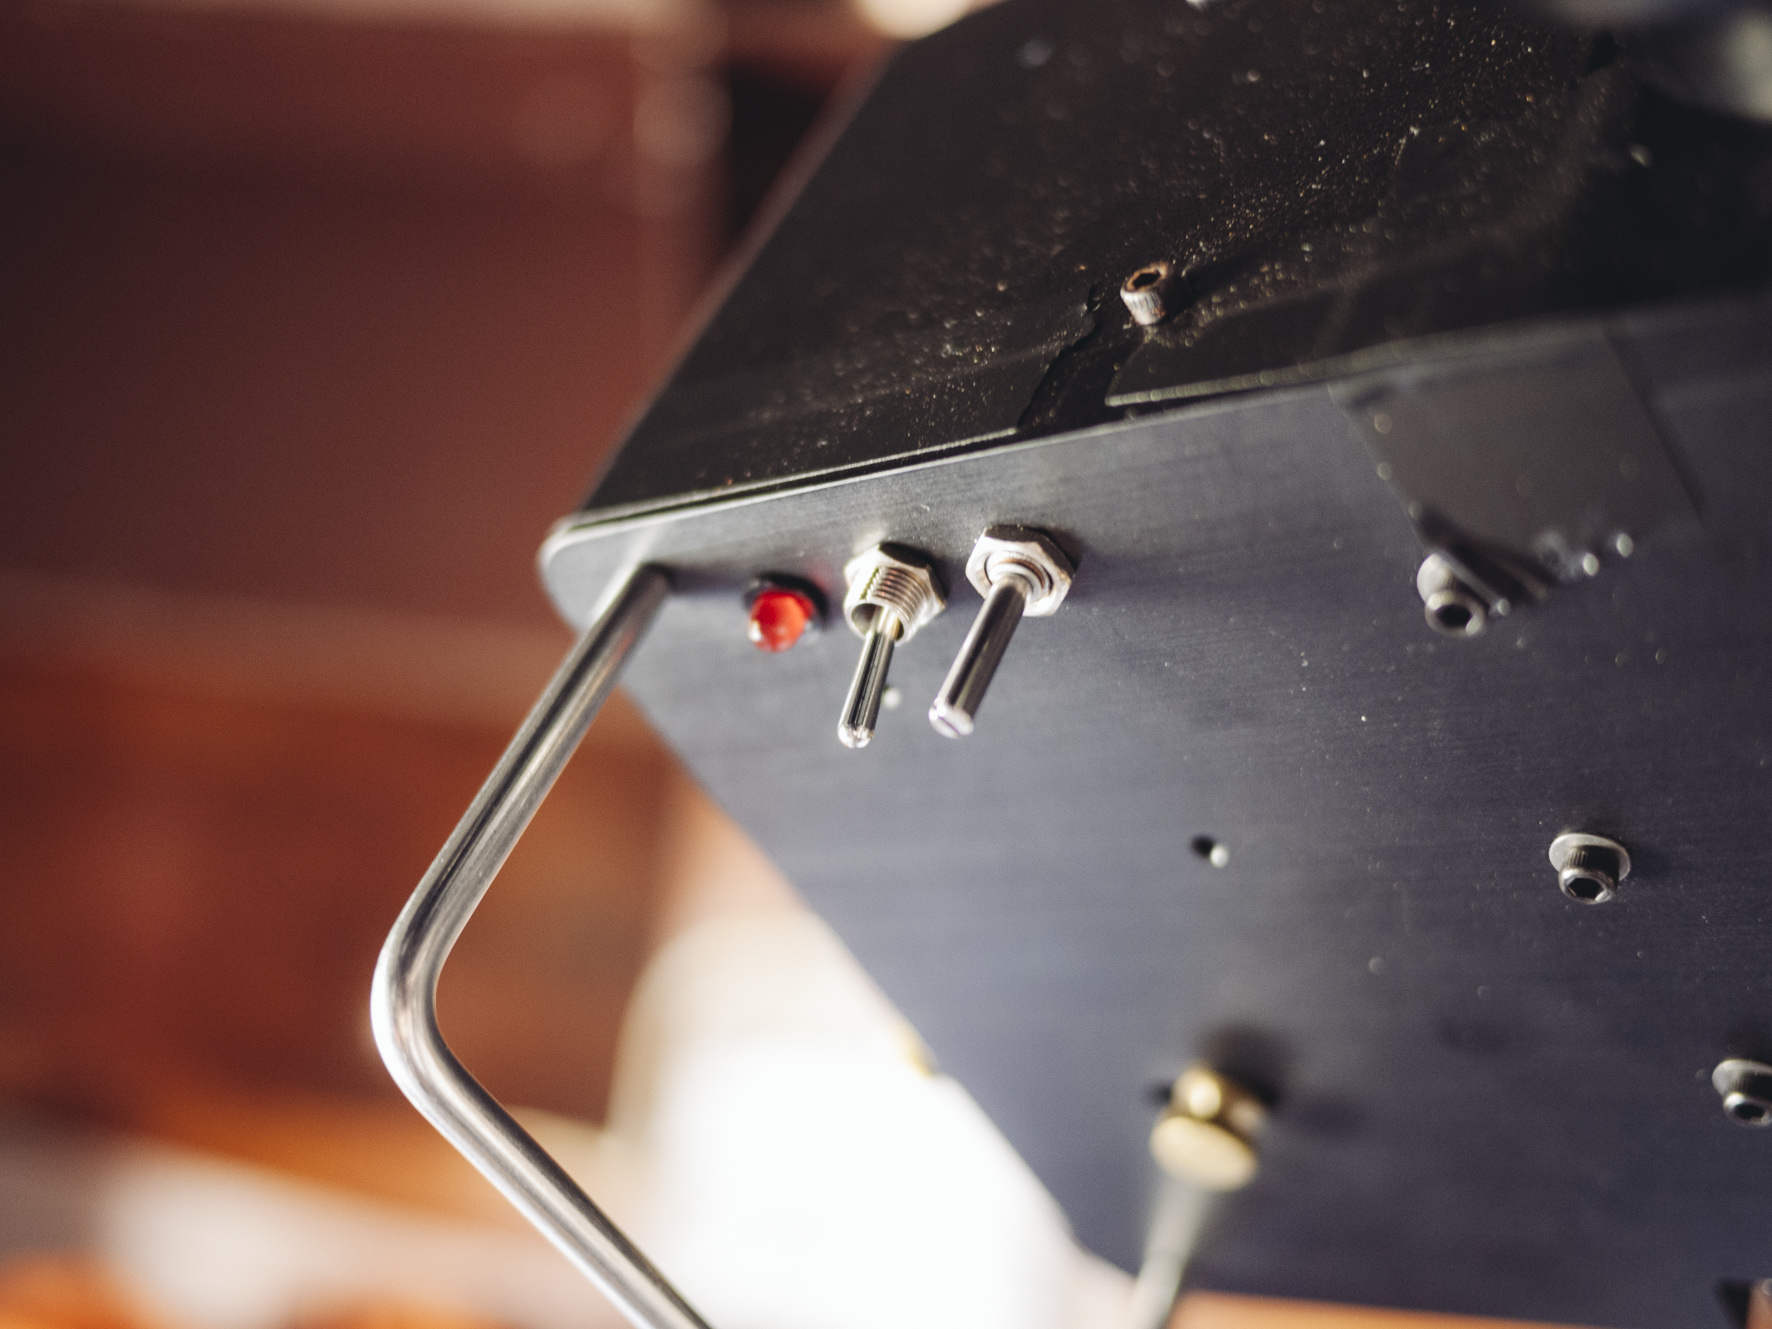
\includegraphics[width=0.49\textwidth]{documentation_images/internal_LED.jpg}
    %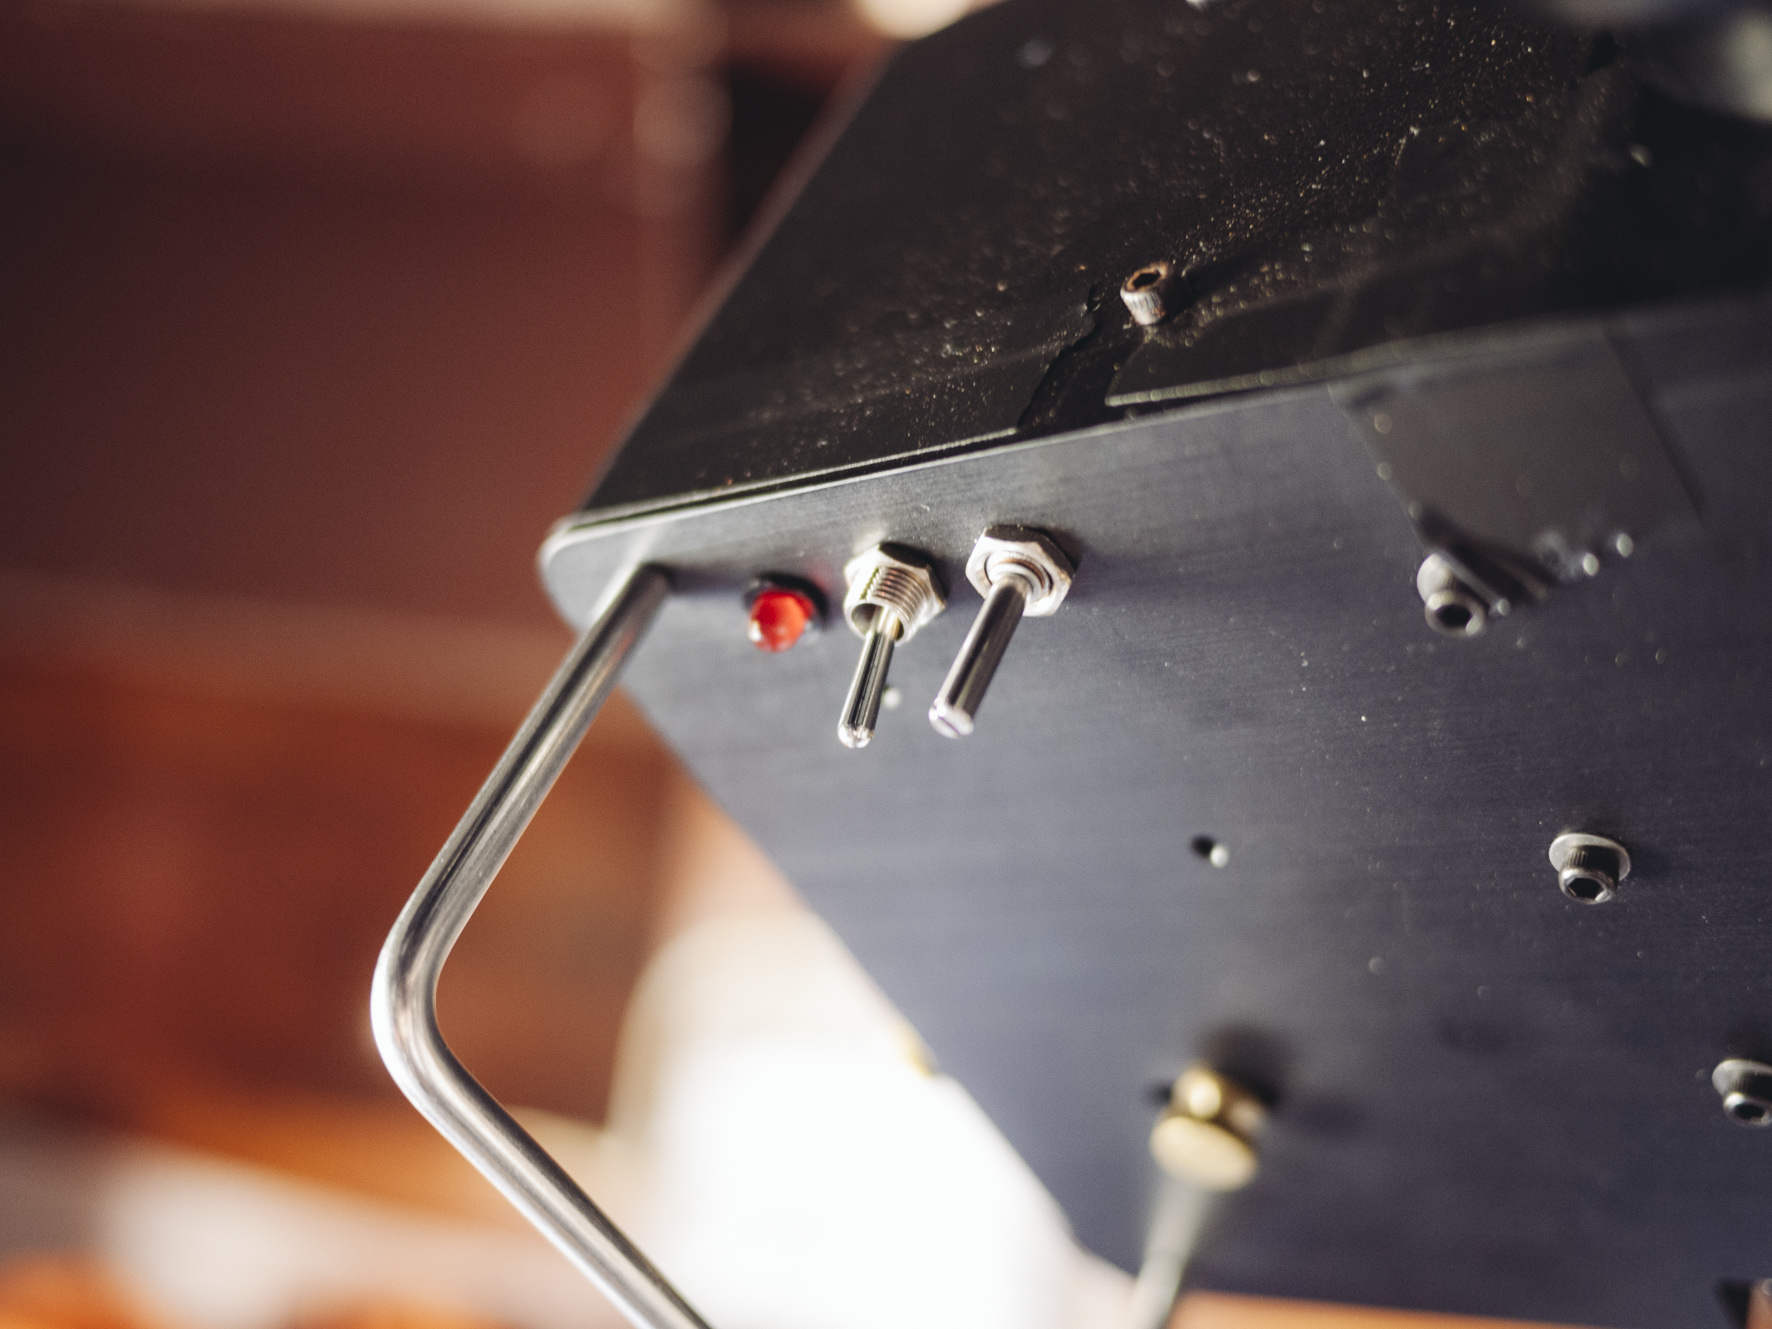
\includegraphics[width=0.49\textwidth]{documentation_images/internal_LED.jpg}
    \caption{\label{fig:autoguide}The `Autoguide' section in The SkyX}
 \end{figure}

 \item click
 \item click
 \item click
 \item `Autoguiding'

\end{enumerate}


\section{Taking spectra}

You are now ready to collect spectra of your chosen object.

\begin{enumerate}
 \item Switch to the `Camera' tab.
 \item Set up series
 \item Expose
 \item done
\end{enumerate}

\section{Standard Spectrographic Stars for Calibration}

To do a detailed study spectrographic data of the object you are investigating, it is necessary to compare it against stars whose spectral characteristics are known. You will therefore need to also collect spectra from a standard spectrographic star during the same observation run. Ideally, this star would be located such that you will view it through the same airmass as the star or object you are investigating.\\

\textbf{A0} (or early A-type) and \textbf{B5} (or late B-type) stars have absorption-line characteristics that make them suitable calibration targets. Search the Simbad catalogue at \\ {\tt http://simbad.u-strasbg.fr/simbad/} for a suitable star in the right part of the sky and collect data for that star like you would for your science target. During the reduction process later, you will apply corrections to the data you collected of the calibration target so that it matches the star's known characteristics. You will then apply those same corrections to the data for the object you are observing. If done successfully, your data will then be both calibrated for wavelength and flux, and you can start investigating the properties of your science target.

%\section{Wavelength and Flux Calibration}



%--------------------------------
% AstroImageJ
%--------------------------------

\chapter{Basic image reduction with AstroImageJ}

AstroImageJ is a version of the open source Java image processing and analysis program ImageJ. The program contains customised plugins and macros that enables working with astronomical images and data.

\section{Installation}
Java must be installed on your system before running AstroImageJ. If your operating system can support it, it is highly recommended that you install Java 64-bit. You can download Java from {\tt http://www.java.com/en/download/manual.jsp}.\\

AstroImageJ for Windows, Mac and Linux can be downloaded from\\
{\tt http://www.astro.louisville.edu/software/astroimagej/}\\

A comprehensive user guide is also available online. This can be found at\\
{\tt http://www.astro.louisville.edu/software/astroimagej/guide/}

\section{Making master calibration files}
Master calibration files are the result of combining the calibration files you took during an observation session (see Section~\ref{calibration}). These are needed any time you want to reduce or process images. AstroImageJ includes a Data Processing module that makes the creation of master calibration images fairly simple.\\

To access the data processing module, click on the `DP' button in the top toolbar, as shown in Figure~\ref{fig:AIJtoolbar}.

\begin{figure}[ht]
  \centering
    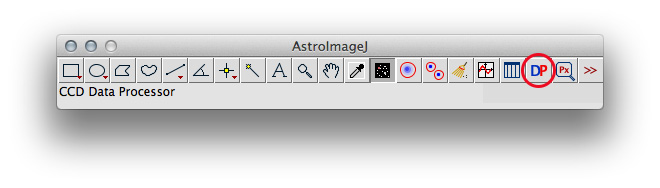
\includegraphics[width=0.75\textwidth]{documentation_images/AIJtoolbar.jpg}
    \caption{\label{fig:AIJtoolbar}The Data Processing button on the AstroImageJ toolbar}
 \end{figure}

 This will open the Data Processing module, the window shown in Figure~\ref{fig:AIJ_DP} below. Ignore the `Science Image Processing' section for the moment and move ahead to the section titles `Bias Subtraction'. Tick both the \textbf{Build} and \textbf{Enable} boxes, since you will be creating your master bias frame afresh and subtract it from the dark frames in the next section. Make sure to select the \textbf{ave} button. AstroImageJ will add all your bias images together and then average them out to remove unwanted noise.\\

\begin{figure}[ht]
  \centering
    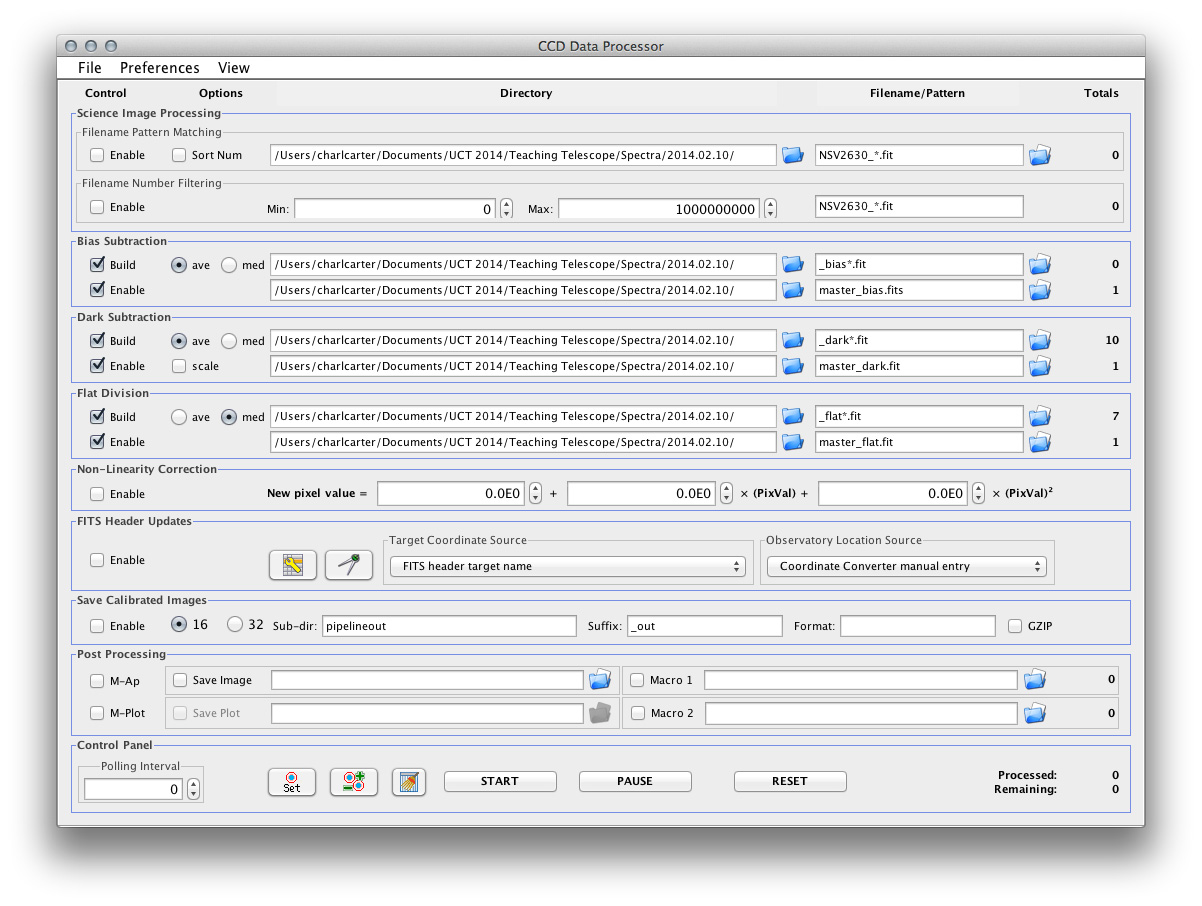
\includegraphics[width=0.94\textwidth]{documentation_images/AIJ_DPwindow.jpg}
    \caption{\label{fig:AIJ_DP}The Data Processing module in AstroImageJ}
 \end{figure}

In the top text field of the two middle fields, enter the path to where your bias images are stored, or use the blue folder icon to browse to the correct folder. In the text box below that, enter or choose where to store your final master image. In the text boxes on the right, you should enter a prefix, suffix or other naming convention by which AstroImageJ can find your raw bias images. You can use an asterisk (*) as a wildcard character. In Figure~\ref{fig:AIJ_DP} any {\tt .FITS} image named `\emph{something}\_bias.fit' will automatically be found. Enter a name for your master bias file in the last box on the right.\\

The same procedure applies for the `Dark Subtraction' and `Flat Division' sections, although in the section for flats, make sure to select the \textbf{med} button instead. This will median-combine the raw flat images instead of averaging them out.\\

One way to check that the right images are selected to be processed, is by verifying that the number in the `Totals' column matches the number of (bias, dark or flat) images in your folder.\\

With the bias, dark and flats sections filled, click on the \textbf{Start} button at the bottom and watch AstroImageJ do it's thing. The master bias image will be created first and then used to process the dark and flat images. A separate window will also appear, reporting on the progress and whether the build was successful or not.\\

To repeat the process for any additional flats (for other filters, for instance), you can uncheck the \textbf{Build} option in the Bias and Subtraction sections, since the masters have now been built already. Select where your other raw flats are stored, enter a unique name for the master and click on \textbf{Start}.

\section{Calibrating Images}

You are now ready to calibrate your science images. Deselect the \textbf{Build} option for the bias, dark and flats, but leave the \textbf{Enable} box ticked. In the top section called `Science Image Processing', select \textbf{Enable}, browse to the folder where your raw images are stores and enter a name pattern for AstroImageJ to search for. You can also instruct AstroImageJ to sort your raw images numerically, and tell the software to only process a certain number range. This could be handy, for instance, when a certain range in your science images are taken with a different filter and you want to divide by the appropriate master flat field.\\

Make doubly sure you have the right master flat field selected, then select the \textbf{Enable} box in the `Save Calibrated Images' (you will forget this at least once!). In this section you should also specify a separate folder (if you wish) and suffix for your calibrated images to distinguish them from the raw ones. Click on \textbf{Start} and watch AstroImageJ run!

\section{Combining Images}
\label{combining}

With all the science images calibrated, the last step is to now combine your image into one higher-quality image. This is sometimes also referred to as `stacking'. The process may seem a bit obscure, but is actually very easy.\\

Open the images you would like to stack by going to \emph{`File -- Import -- Image Sequence...'}. As before, you can filter these by name and/or number. Select only the images that have been calibrated and also only select images from one specific filter at a time. You will be making a kind of `master' image per filter, i.e. a final stacked and calibrated red or blue or luminance image, for example.\\

Depending on how much memory your computer has available to Java, you can open the stack in one of two ways: By default, opening a stack loads all the images in the stack into your computer's memory. Alternatively, if you select the `virtual stack' option, only the image you are currently viewing (i.e. the one at the front of the stack) is loaded into memory. This may slow processing the stack down a bit, but frees up memory for other applications and prevents `out of memory' errors.\\

Make sure the AstroImageJ toolbar is \textbf{on top} of your image sequence window. That is, the main menu should read \emph{File / Edit / Image / etc} and not something else. You may now want to normalize your images to get the background level the same. This is as easy as going to \emph{Process -- Normalise}.\\ 

Now to combine you images, select \emph{Image -- Stacks -- Z Project}. And that's it! You can save the result as a new {\tt .FITS} image. You might want to also save a copy as a {\tt .PNG} or {\tt .JPEG} to use as new desktop background or Facebook cover photo.\\

Combining images from different filters into `master'-filter images like you have done above, will allow you to later use other image manipulation software, like Adobe Photoshop or Gimp, to produce a final colored image to use for scientific analysis or to show off to friends and family.

\subsection{Aligning images}

If the result combining your images appears to have multiple instances of every star or just looks completely wrong, it might be that the images are not properly aligned. This can happen due to the telescope's tracking not being perfect, or small bumps or jitters to the telescope during your observation run. You will need to specify a few stars in the image that AstroImageJ can then use to align the whole stack.\\

\begin{enumerate}
 \item Open a new {\tt .FITS} image sequence by going to the menu \emph{File / Import / Image Sequence} and specifying which images to import. Check that the number of images selected are correct and un-check \textbf{'Use Virtual Stack'}.
 \item In the image sequence window, click on the 'Align' button (the icon contains three squares stacked on top of each other).
 \item In the window that pops up, deselect the `Remove Background...' option and press \textbf{OK}.
 \item Select some bright stars in your image by left-clicking on them.
 \item With a few stars selected, right-click anywhere in the image to begin the alignment process.
 \item Remember to save the images again after alignment.
\end{enumerate}


\section{Measuring Point Spread Function}
\label{PSF}

Point spread function (PSF) fitting or profile fitting is used when the star field in an image is too crowded to do simple aperture photometry. PSF fitting uses model signals and fits them to the data in your image. Usually the PSF has the shape of point sources, like stars, in the analysed image. Stellar images are usually fitted with a radial Gaussian intensity profile, and the flux of the target is defined by the fitted model curve.\\

PSF fitting is possible in AstroImageJ using the `Multiple Aperture' tool. This tool is accessible from the main toolbar in AIJ, as shown below in Figure~\ref{fig:AIJ_MA}.

\begin{figure}[ht]
  \centering
    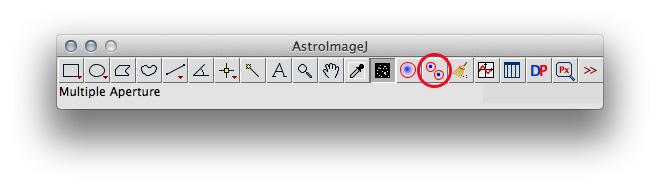
\includegraphics[width=0.94\textwidth]{documentation_images/AIJtoolbarMA.jpg}
    \caption{\label{fig:AIJ_MA}Accessing the `Multiple Aperture' tools in AstroImageJ}
 \end{figure}

You will however first have to import the stack of images you would like to do photometry on. This can be done by going to \emph{`File -- Import -- Image Sequence...'} and selecting the correct images. For accurate measurements, it is important that these image have been properly calibrated as described above. Depending on the memory your computer has available to Java, you may want to select the \emph{`Use Virtual Stack'} option. It is a it slower 


\section{Photometry in AstroImageJ}
\label{AIJ_Photometry}
Aperture photometry can be performed in AstroImageJ on a stack of calibrated and aligned images. Essentially, you want to extract source and background counts from and image of a star field. The process is briefly described below.

\begin{enumerate}
 \item Open the stack of images you would like to perform photometry on as described above in Section~\ref{PSF} and check the \emph{`Use Virtual Stack'} option.
 \item To begin photometry you should now select the target and comparison stars with suitable photometric circles. To calculate the FWHM of your star and set up an appropriate profile for your target, do the following:

  \begin{itemize}
   \item From the main menu select the line tool (see Figure~\ref{fig:linetool}.)

  \begin{figure}[ht]
  \centering
    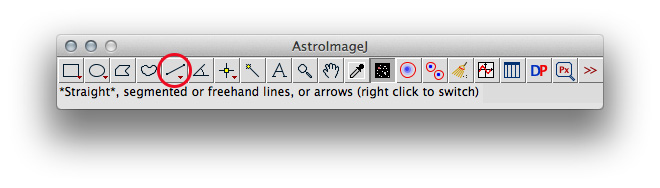
\includegraphics[width=0.94\textwidth]{documentation_images/AIJlinetool.jpg}
    \caption{\label{fig:linetool}The line tool on the main AstroImageJ menu}
 \end{figure}

   \item In the image window, draw a line through your target.
   \item Then select \emph{Analyze -- Plot seeing profile} and press 'OK' on the popup window.
   \item This will create a profile of your target and calculate it's FWHM. This profile saved automatically, so you can close this window and the graph again.
  \end{itemize}

 \item Select the 'Multiple Aperture' tool from the main menu.
 \item This will open another window in which the profile you just calculated for your target star should be filled in already. If not, just enter the profile values you found a few steps ago.
 \item Set the target and comparison stars by simply left-clicking on them. Be sure to click on your target first, followed by the comparison stars. You should now have something resembling Figure~\ref{fig:targets}
 \item Right-click anywhere in the window, or just press 'Enter' on your keyboard when you have picked enough stars. This will initialize the photometry process and produce a set of measurements and a light curve plot.
 \item Save your results by selecting \emph{File -- Save All}. This will save a set of files, which are the measurements you just made in an {\tt .xls} file. You you can open and study these measurements further in most popular spreadsheet programs.

  \begin{figure}[ht]
  \centering
    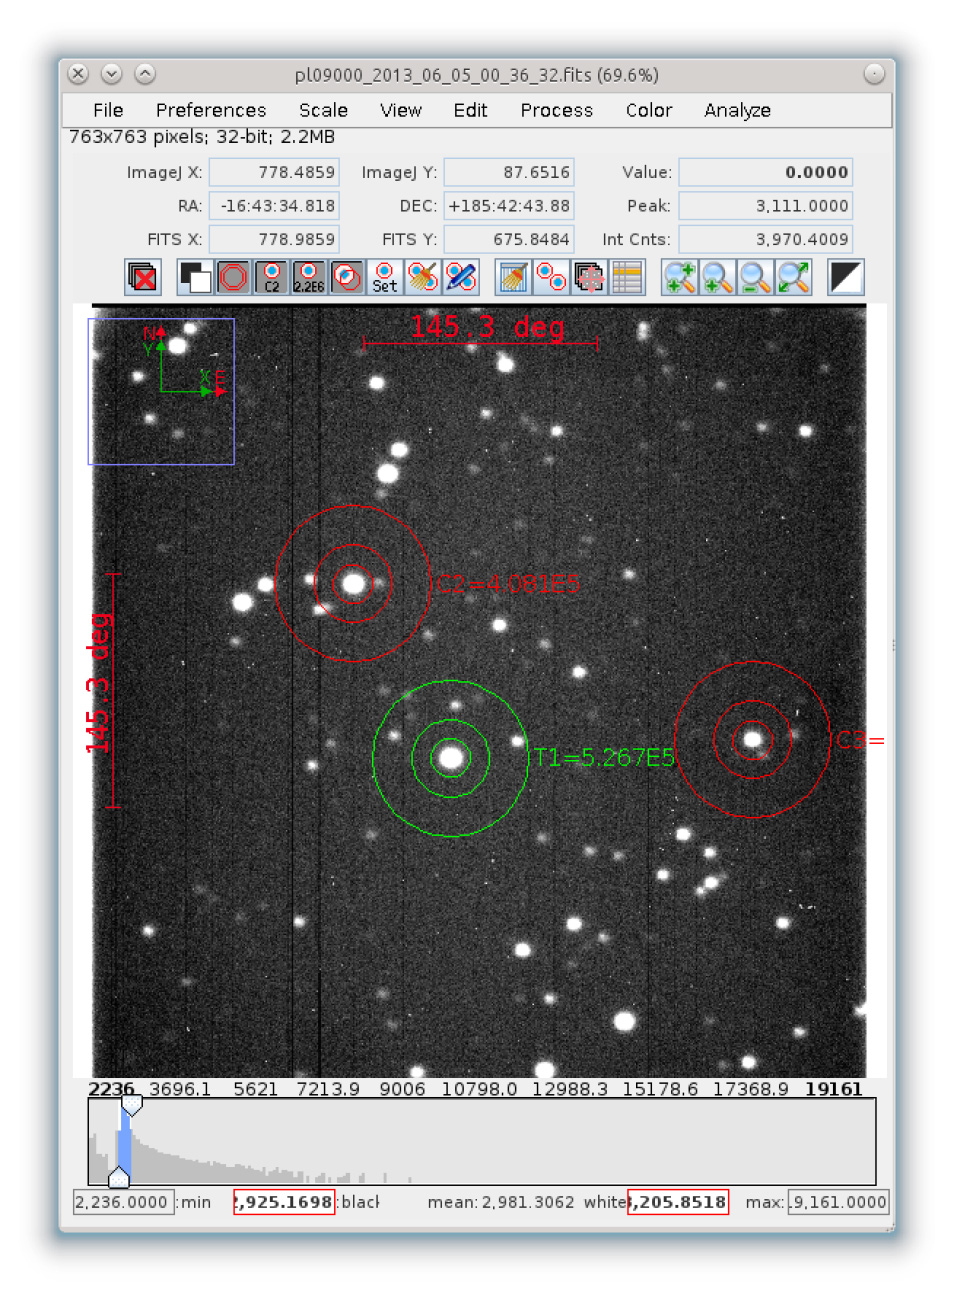
\includegraphics[width=0.55\textwidth]{documentation_images/photometry_targets.jpg}
    \caption{\label{fig:targets}Target and comparison stars selected in the image window}
 \end{figure}
 \end{enumerate}

The light curve plot you produced above is the flux of the target star divided by the flux of the couple of comparison stars you selected. The use of comparison stars should in principle correct for any variations in atmospheric transparency, like passing clouds. Thus you would ideally not select a comparison star that is itself variable.\\

You can explore plotting options like axis labels and titles from the Multi-Plot button in the main menu.

% \section{Making light curves}

% \section{Plotting results}

\section{Making LRGB images}
Combining images like you have done in Section~\ref{combining} above may produce images and data that is sufficient for data analysis, but, admittedly, they lack the flair and color of the images of deep-space you might be used to seeing. Aside: Visit {\tt http://apod.nasa.gov/apod/astropix.html} for a great selection of deep-sky and other astronomy-related images.)\\

To produce the stunning images we might see from telescopes like the Keck Observatory or Hubble, a few little extra image-processing effort is needed. The exact details differs according to the software you use, but usually entails loading the `master' monochrome images from each filter into a different color channel, and then using these channels to colorise your main luminance image. A careful dose of unsharpening after you are done colorising can give features in the image extra definition.\\

Producing color images is however scientifically useful to, as it provides a way to highlight exactly where, for instance, a could of Hydrogen gas is in a nebula. You might be surprised to learn that most astronomical images are usually not rendered as you would see it with the eye. This is to emphasize certain characteristics, visualize things that would normally be invisible to the human eye like X-rays or UV-light, or produce more aesthetically pleasing images. Figure~\ref{fig:thor} is an example of an image that was taken with the teaching telescope with red, green, blue and H-alpha filters and combined into a final color image.\\

% please replace if we have something better!
\begin{figure}[ht]
  \centering
    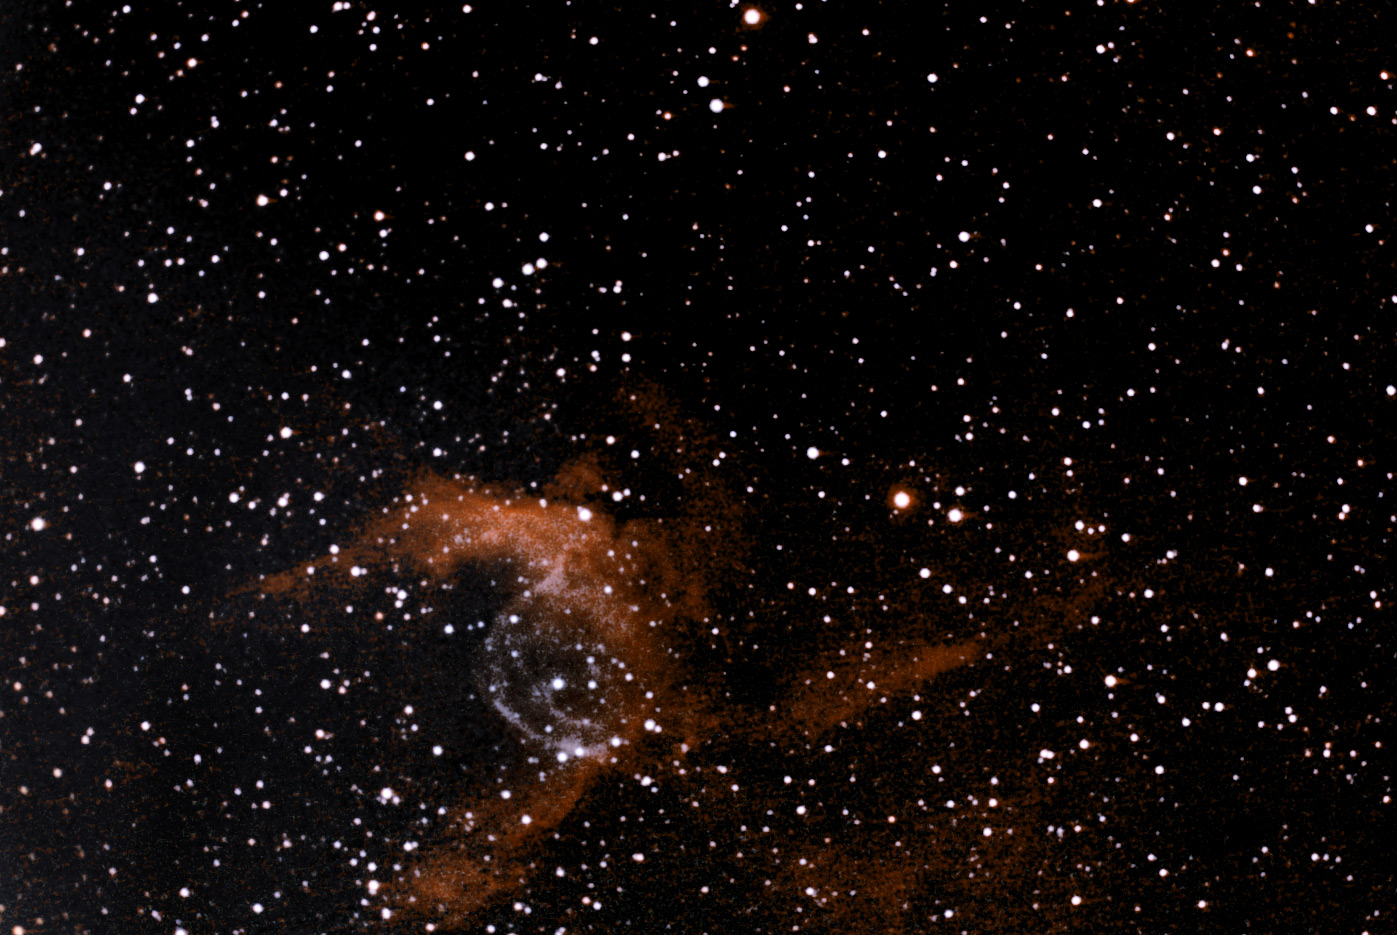
\includegraphics[width=0.75\textwidth]{documentation_images/thors_hat.jpg}
    \caption{\label{fig:thor}The Thor's Hat Nebula as seen by the teaching telescope}
 \end{figure}



% To be expanded with a tut / walkthrough later?

%--------------------------------
% Remote Observing
%--------------------------------

\chapter{Remote observing}

\section{Remote access and Weather considerations}
\label{remote_obs}

Sitting in the dome all night while the telescope integrates is generally not a good idea. 
The temperature differences between your body can cause differences in the seeing in the telescope. 
We have set up a way to access the telescope computer from a remote place, so that the disturbances 
of the telescope are kept to a minimum.\\

To get the remote control software, goto \url{http://www.teamviewer.com/en/} and install 
the software on your computer. To access the observatory computer use the address:\newline
{\tt telescope.ast.uct.ac.za} and password: {\tt bonjour}.\\

Make sure that in the observatory that the telescope wont run into anything 
as it move throughout the night. Sit back in your remote setting and regularly keep an eye 
on the weather conditions. \\

\section{Weather conditions}

Rain, high humidity and excessive wind can cause serious damage to the observatory, the telescope and other instruments. When observing remotely, regularly check on the conditions outside. Should it become increasingly windy, foggy or threatening to rain, it would be best to interrupt the current observation session, park and close the dome and shut down and park telescope.




%--------------------------------
% Advanced Procedures
%--------------------------------

\chapter{Advanced Observation Procedures}

\section{Instrument change}

An assortment of instruments are installed in an instrument stack at the back of the 14-inch Celestron telescope. This includes a rotator, focuser, an adaptive optics module, and a CCD camera. During the course of 2013 a Santa Barbara Instrument Group Self Guided Spectrograph (SBIG-SGS) was added to the suite of instruments at the Tony Fairall Teaching Observatory. This section will describe how to change between the CCD-imager and the spectrograph. While it is not a difficult or laborious process, sufficient care should still be taken when handling these instruments.\\

\subsection{Changing from the CCD-imager to the spectrograph}

Steps to take down the CCD-imager and install the spectrograph are described below.

\begin{enumerate}
 \item If the telescope and camera are connected to the laptop and any software, disconnect the camera, `park' the telescope, and set the RA and DEC drives to their `lock' positions.
 \item Unplug the power, USB and telescope connection plugs from the camera.
 \item On the focuser (the bigger, black disk-like instrument), locate the 4 hex key holes. These are on the outside circumference of the fatter of the two disks.
 \item While supporting the imager, use a $\frac{5}{64}$ hex key to loosen the four bolts. Figure~\ref{fig:change_inst1} They only need to bee loosened and need be not removed completely.

\begin{figure}[ht]
  \centering
    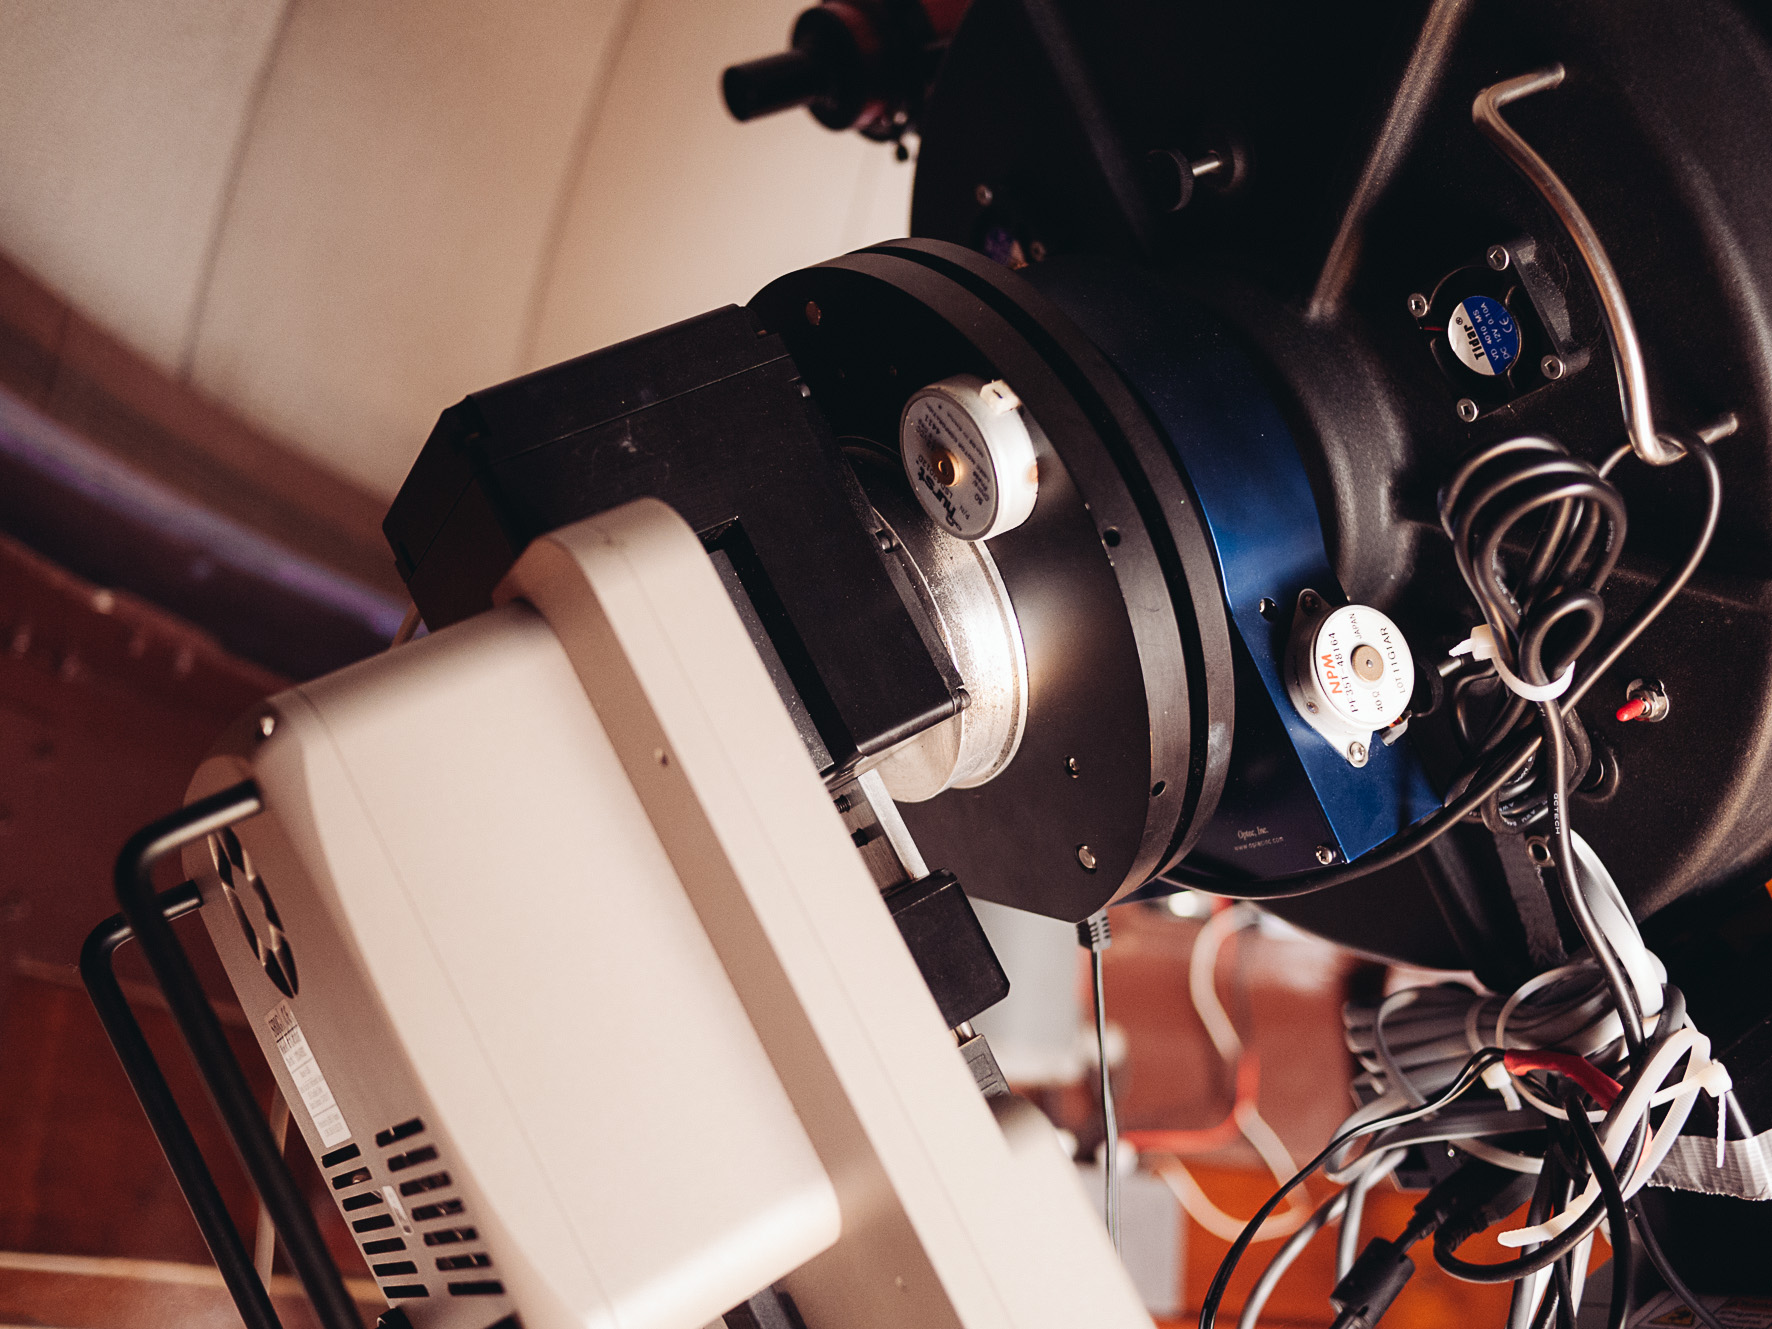
\includegraphics[width=0.49\textwidth]{documentation_images/change_inst1.jpg}
    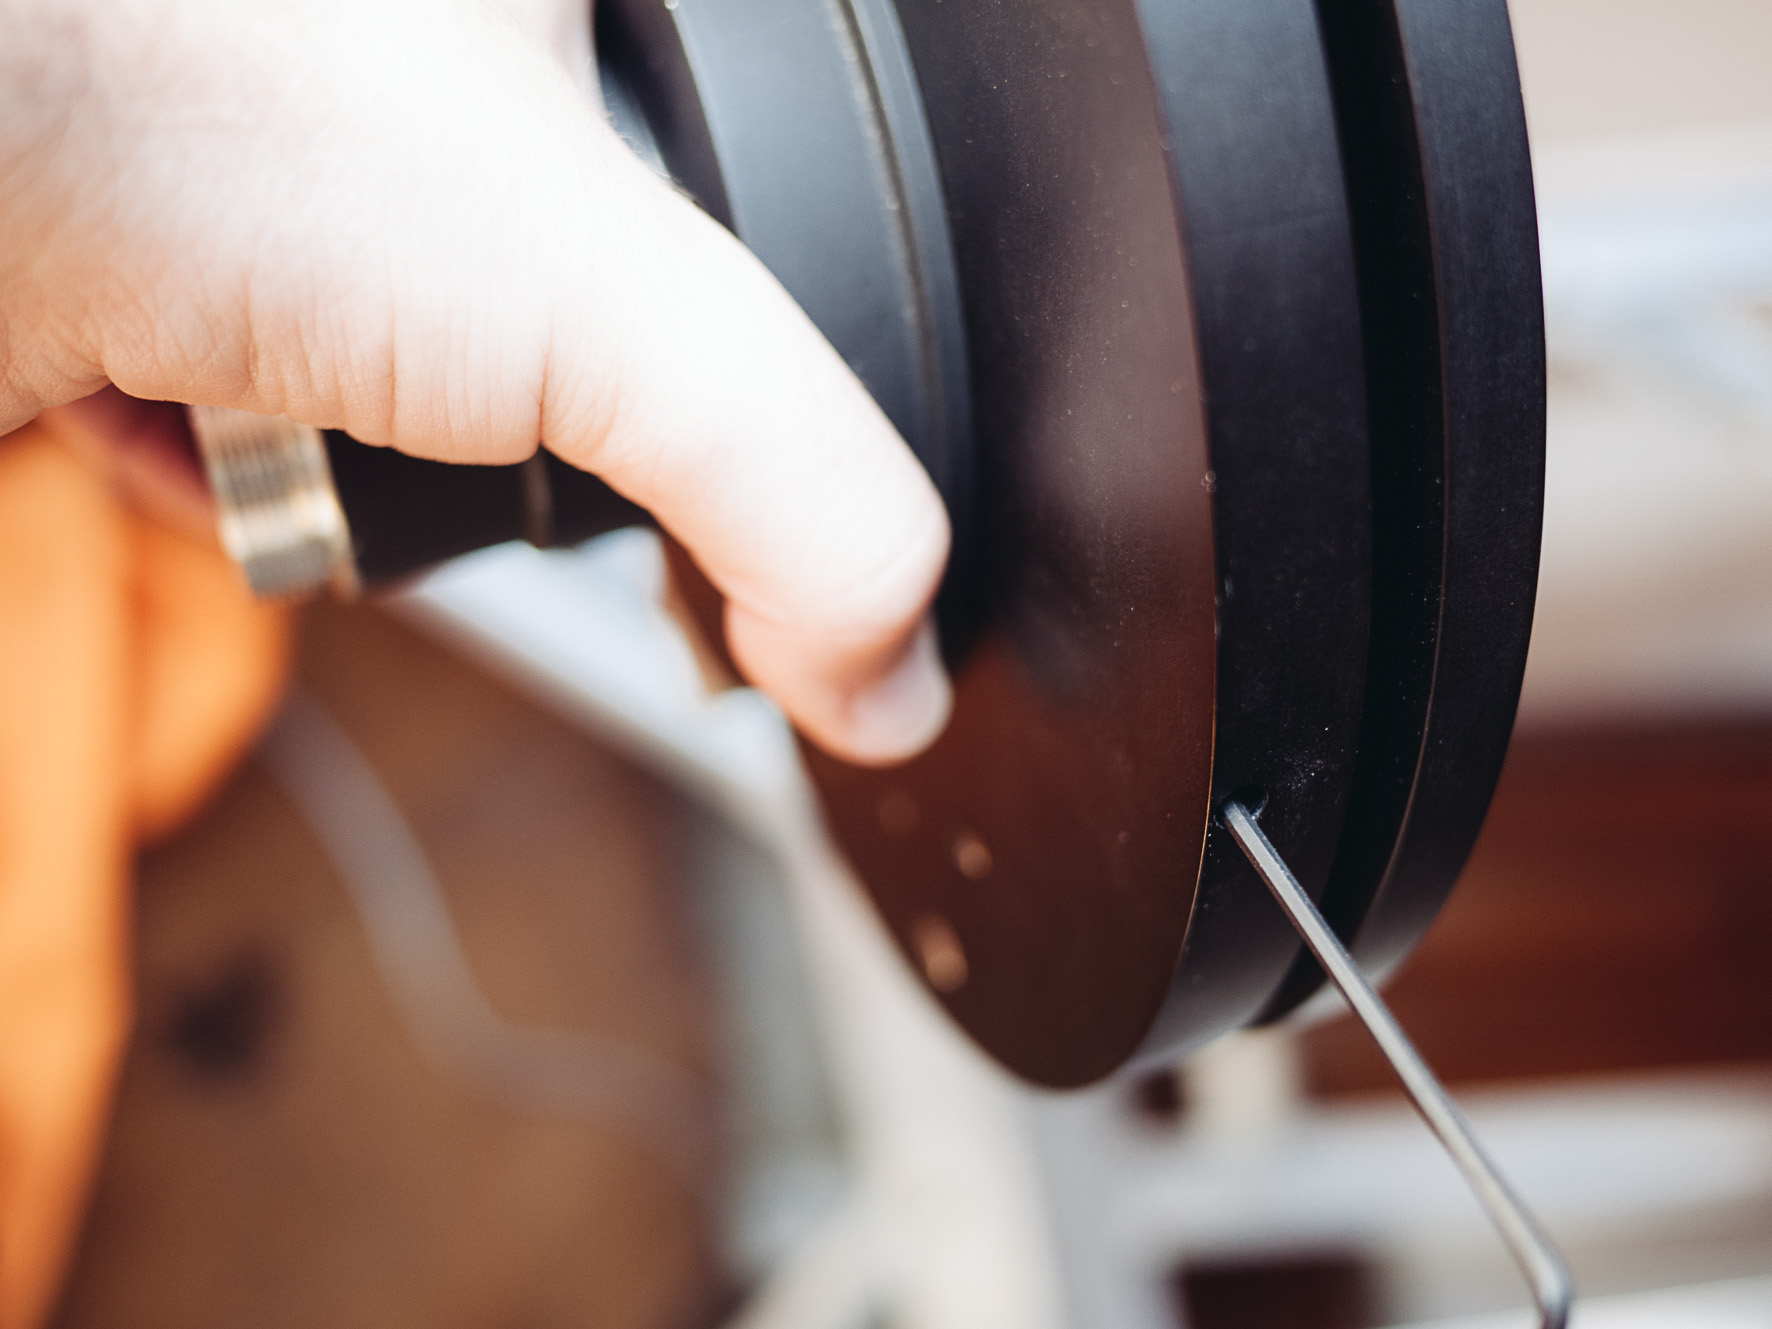
\includegraphics[width=0.49\textwidth]{documentation_images/change_inst2.jpg}
    \caption{\label{fig:change_inst1} The instrument stack with imager, and the location of a bolt on the focuser.}
 \end{figure}

 \item When three or all of the bolts are sufficiently loose, the imager should come away from the focuser without any effort.
 \item In the black adaptive optics module attached to the imager, you will see a round lens. This is a focal reducer. Note the focal reducer's orientation, with the \emph{convex} side of the lens pointing \emph{out} as seen in Figure~\ref{fig:change_inst3}.

 \begin{figure}[ht]
  \centering
    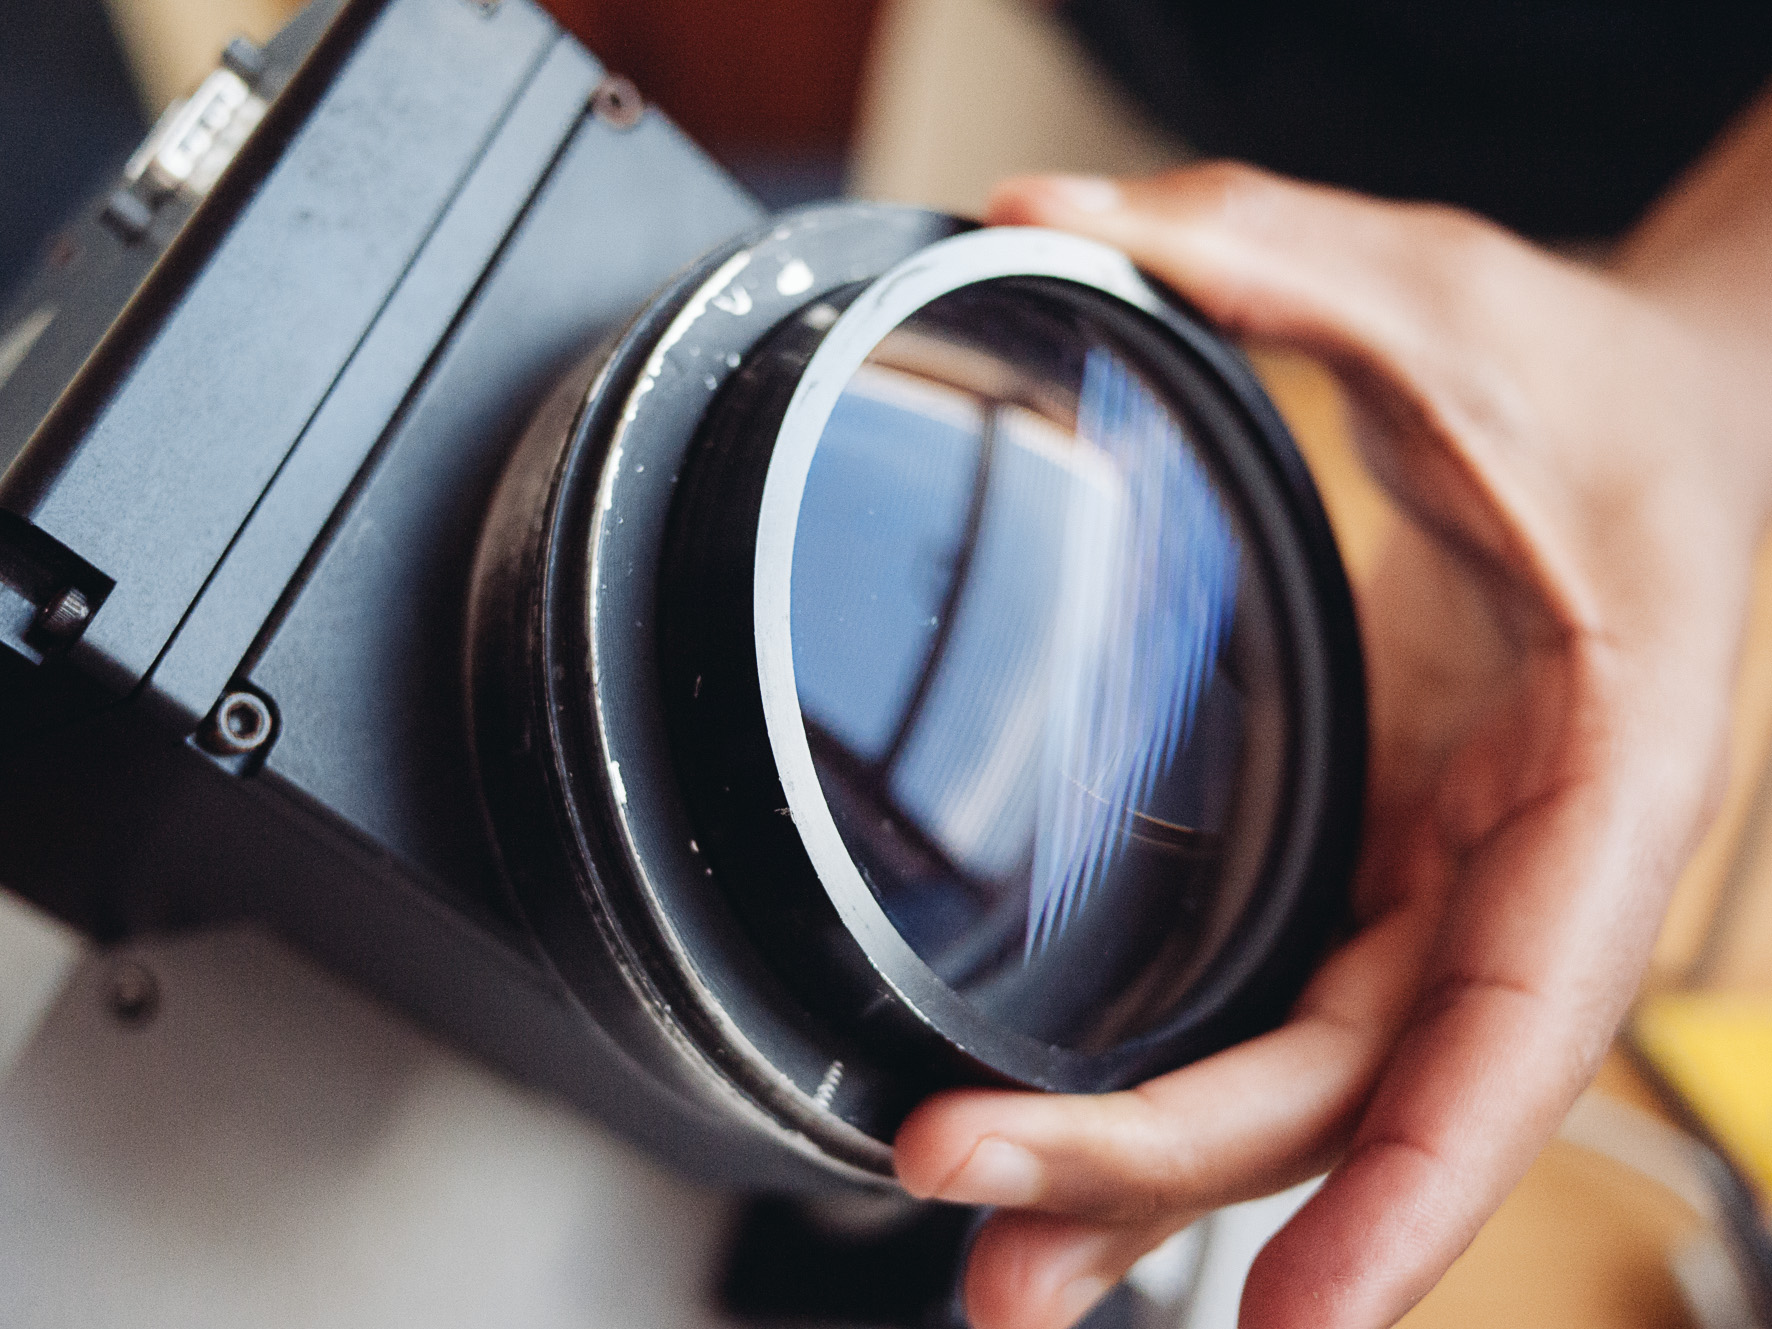
\includegraphics[width=0.49\textwidth]{documentation_images/change_inst3.jpg}
    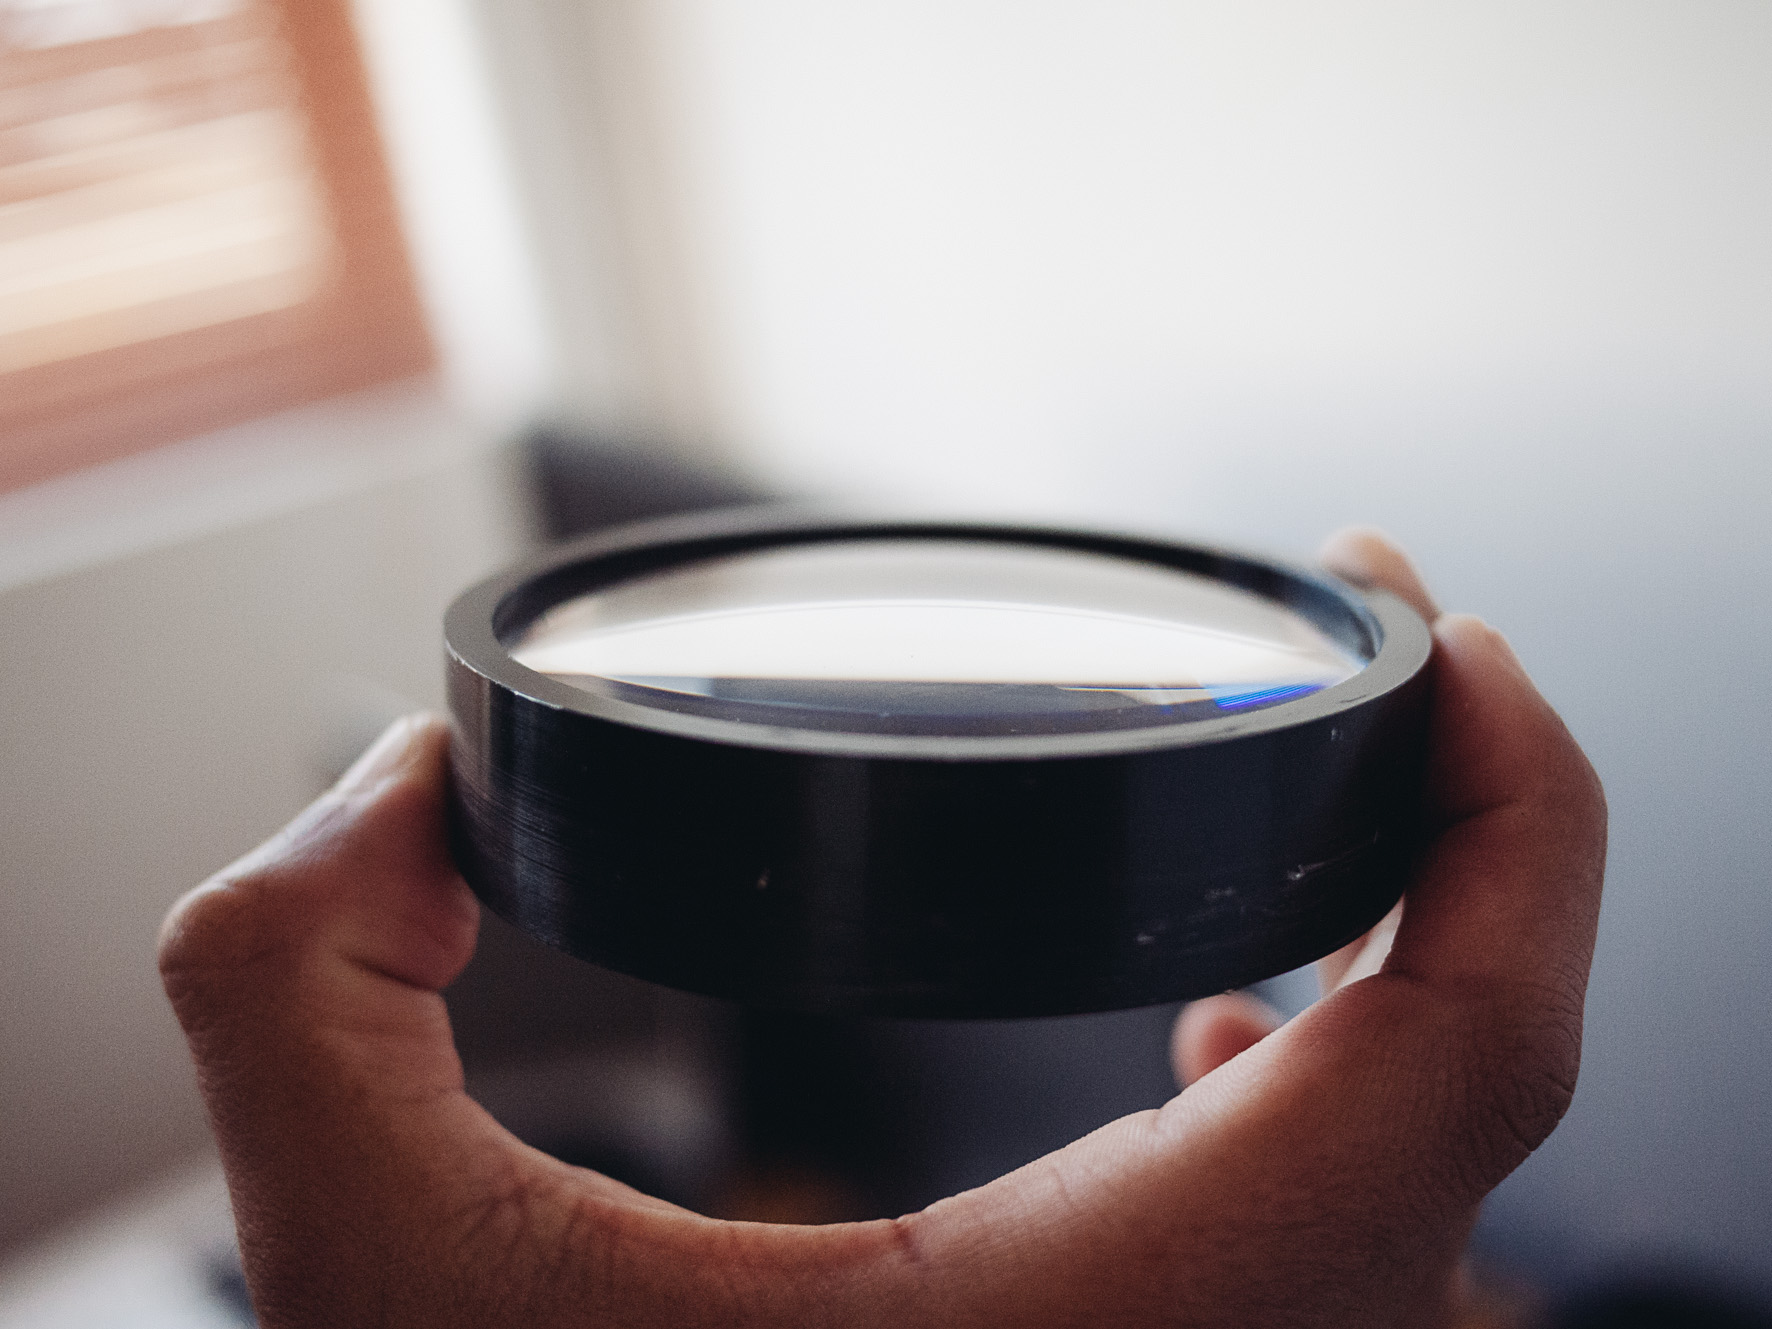
\includegraphics[width=0.49\textwidth]{documentation_images/change_inst4.jpg}
    \caption{\label{fig:change_inst3} Focal reducer -- note the convex side pointing out.}
 \end{figure}

 \item Set the imager aside out of harm's way, gently lift out the focal reducer from the AO-module and place it in the receptive nose piece of the spectrograph. Again, make sure you put it in the right way around.
 \item You can now attach the spectrograph to the instrument stack -- keeping the nose piece flush with the side of the focuser, tighten the four bolts on the focuser.
 \item Perform a `pull test' to double check that everything is tightened sufficiently.
 \item You can now plug in the power, USB and telescope control plugs into the camera at the back of the spectrograph. These plugs are shown in Figure~\ref{fig:change_inst5}
 \item Lastly, you may need to rebalance the telescope to ensure it moves properly. Put the DEC drive on `balance' mode and swing the telescope so that it and the weight bar lie horizontally. Then, adjust the innermost weight until the the telescope can remain perfectly still without any assistance. The spectrograph is now installed and ready to analyze some starlight!

  \begin{figure}[ht]
  \centering
    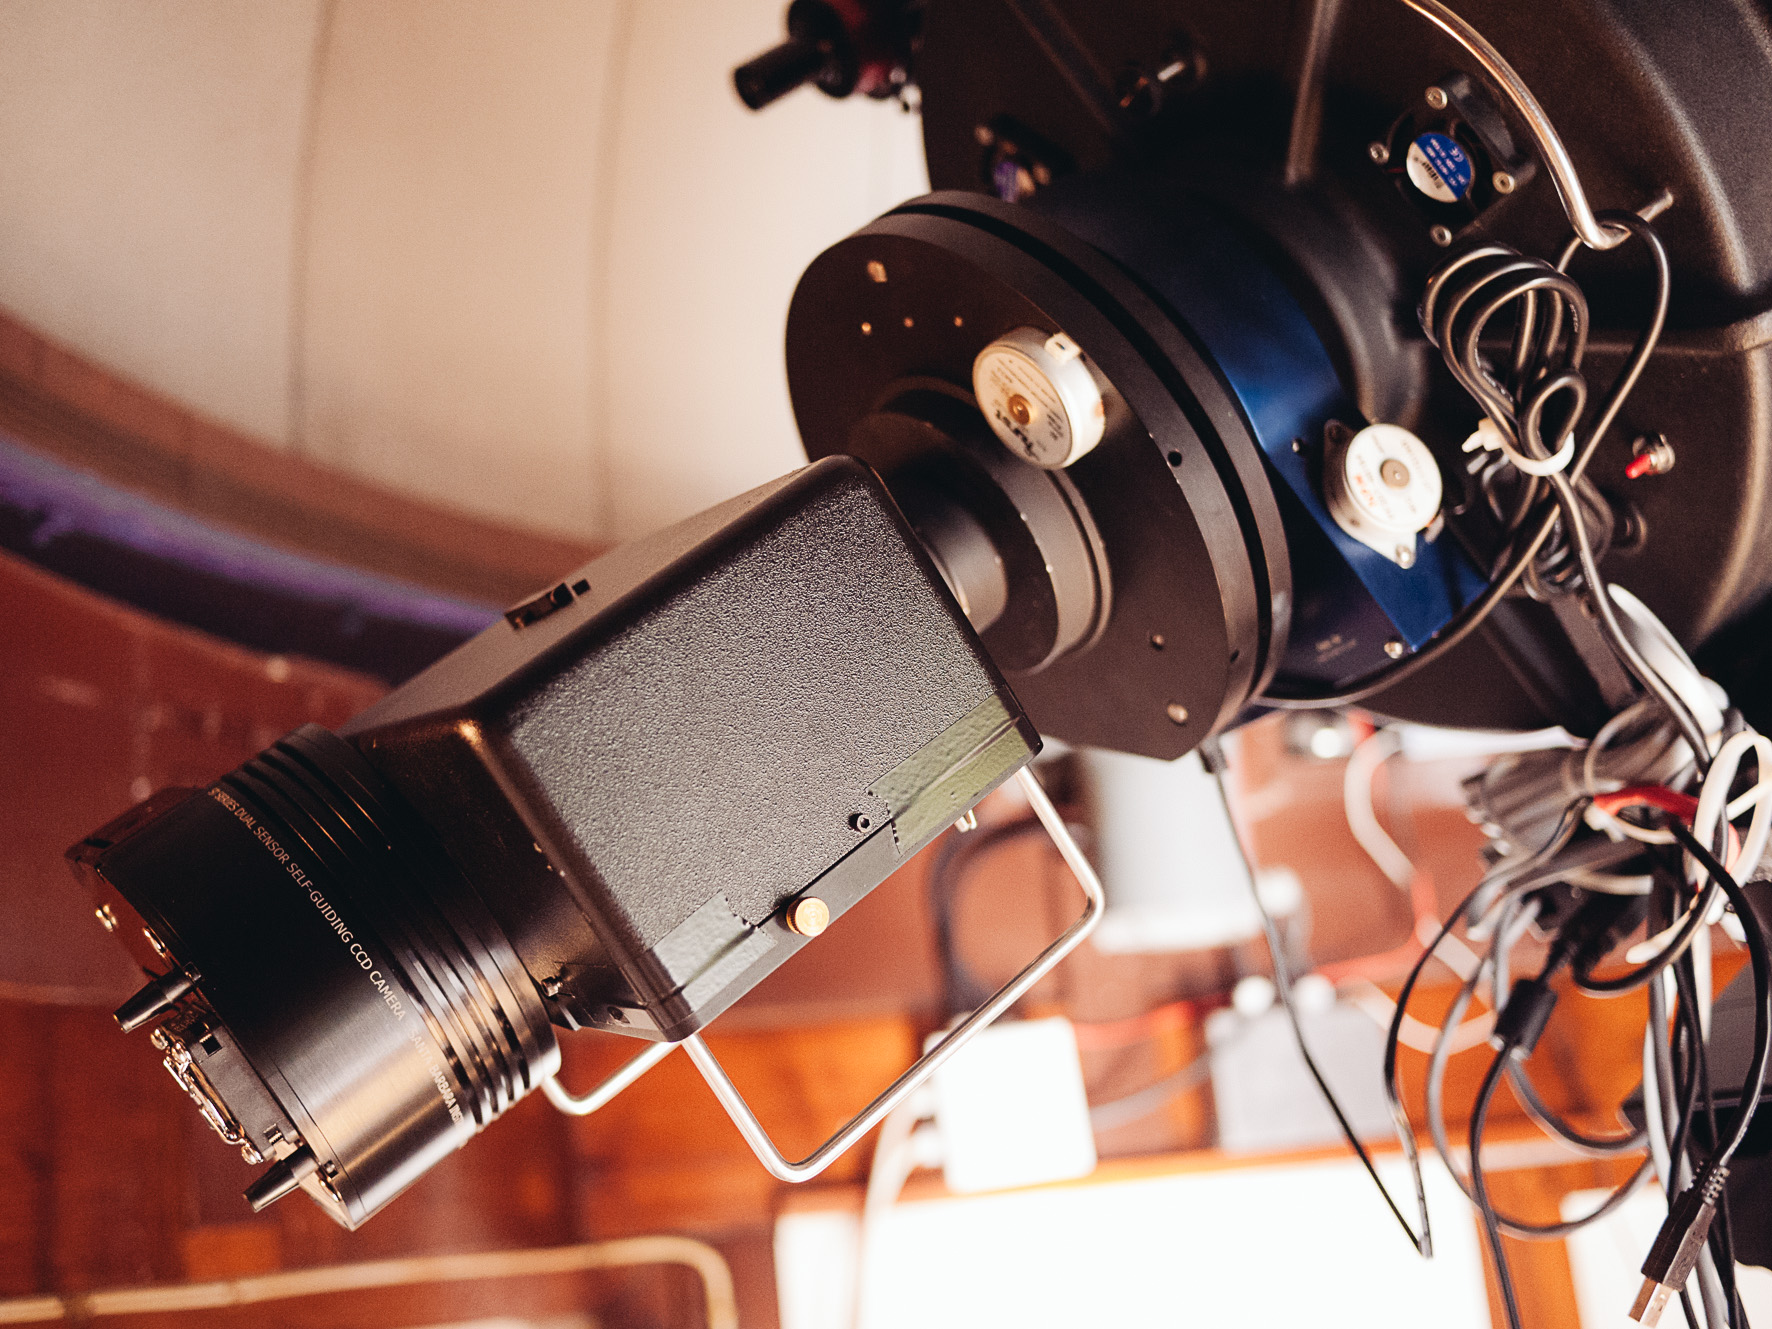
\includegraphics[width=0.49\textwidth]{documentation_images/change_inst5.jpg}
    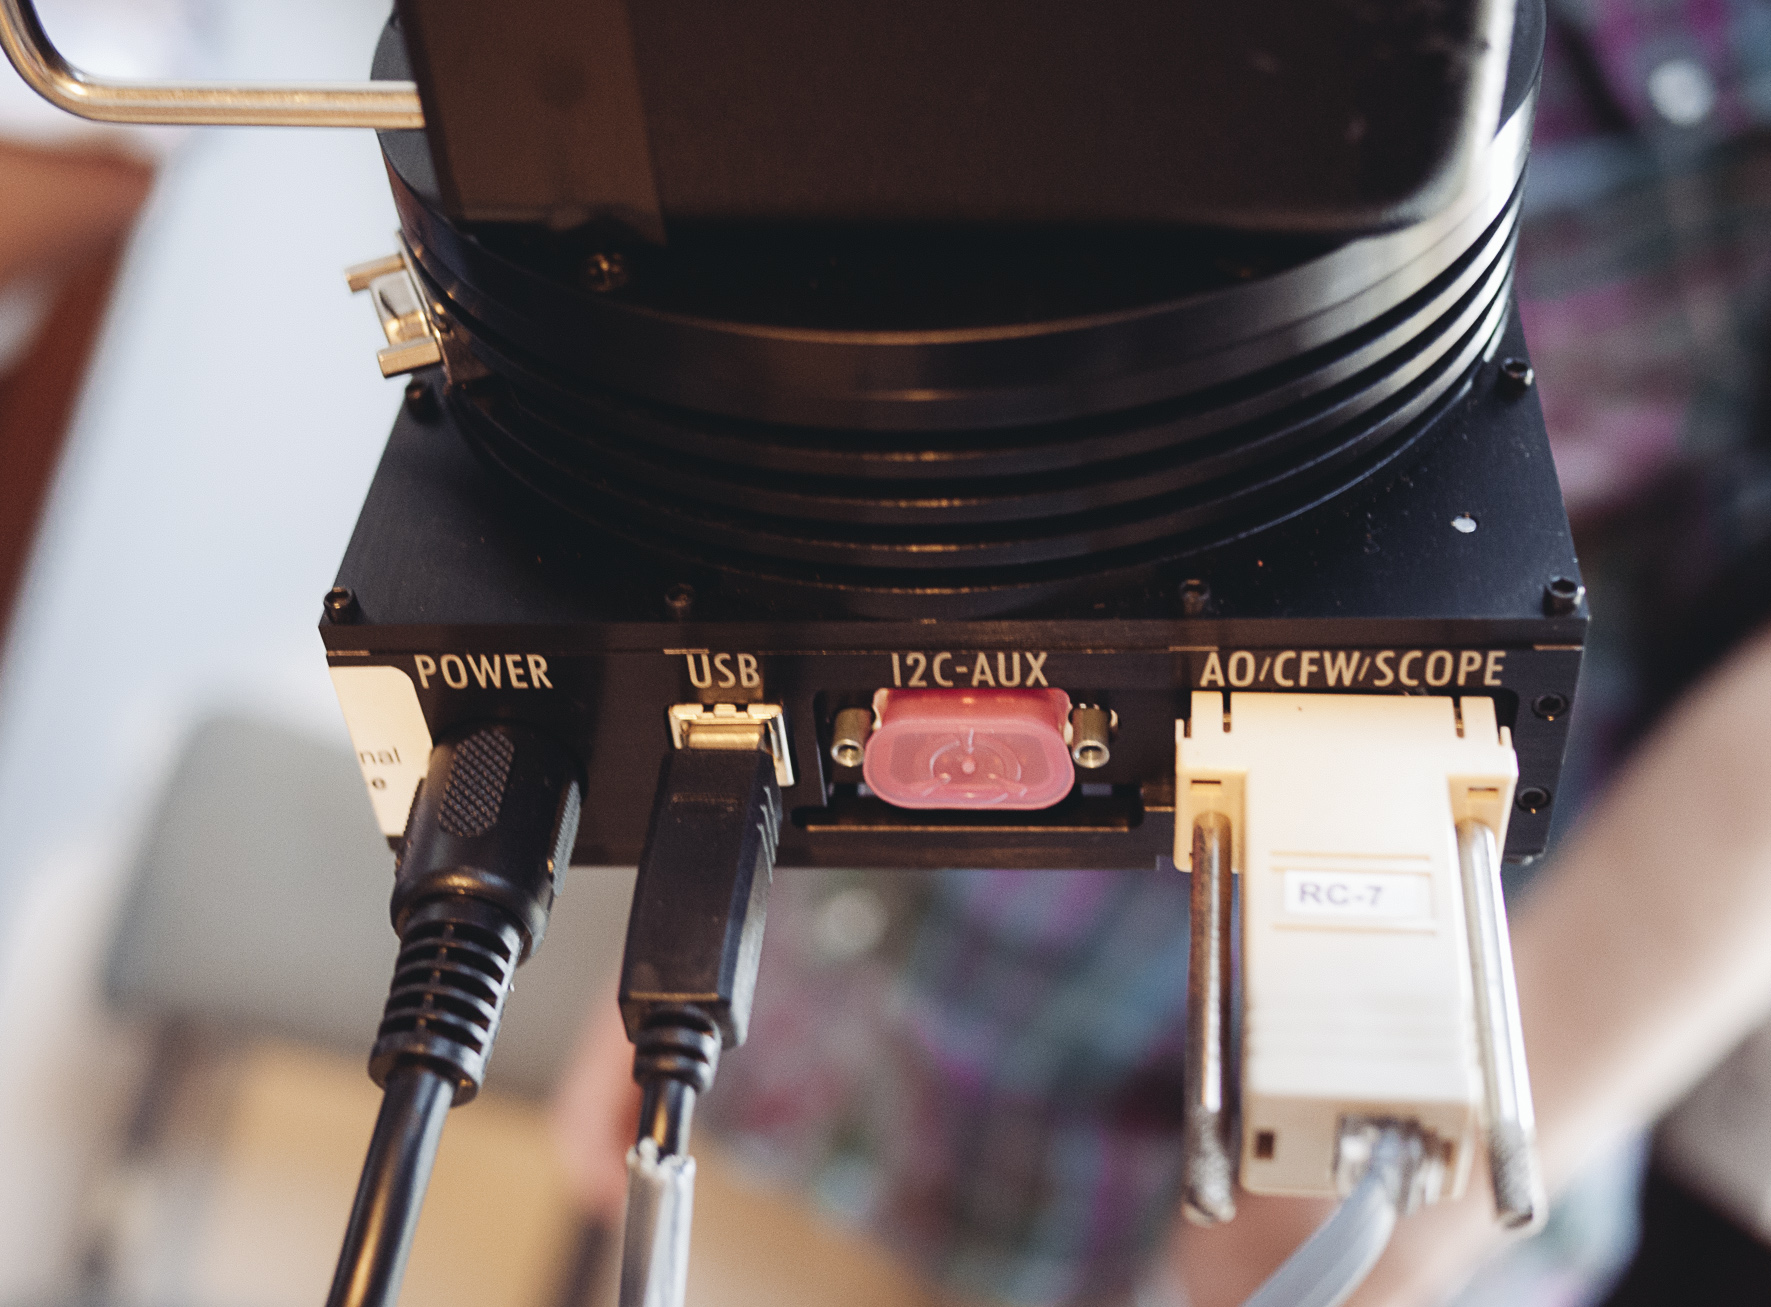
\includegraphics[width=0.49\textwidth]{documentation_images/change_inst6.jpg}
    \caption{\label{fig:change_inst5} Spectrogaph installed on the telescope, and the spectrographs's plugs.}
 \end{figure}

\end{enumerate}



\subsection{Changing from the spectrograph to the CCD-imager}

The procedure for taking down the spectrograph and installing the CCD camera is almost exactly the same as for the other way round, only this time you end with a camera attached to the telescope (surprise!). As before, take care with the focal reducer and perform a `pull test' when you're done to make sure everything is sturdy.

\subsection{Maintenance}

\subsection{Mosaics}




%--------------------------------
% Automatic Reduction API
%--------------------------------

\chapter{Automatic Reduction API}
\label{autoapi}




%--------------------------------
% Troubleshooting
%--------------------------------
\chapter{Troubleshooting}
In case of any problems, shut down the telescope and email Thuso at {\tt thuso@ast.uct.ac.za}

%\appendix
%\chapter{A}

\end{document}
